\chapter{Supplements: FLUX.1 {[dev]} Experiments}

\section{Experimental Default Setup}

Fig. \ref{fig:ArchSingleBlockComp} and Fig. \ref{fig:ArchDoubleBlockComp} provide an overview of the individual components within the double- and single-stream blocks of FLUX.1 [dev] which are subject to \gls{SVD} compression. Additionally, Tab. \ref{tab:flux_training_config} provides the training settings for FLUX.1 {[dev]}.
\begin{figure}[H]
	\centering
	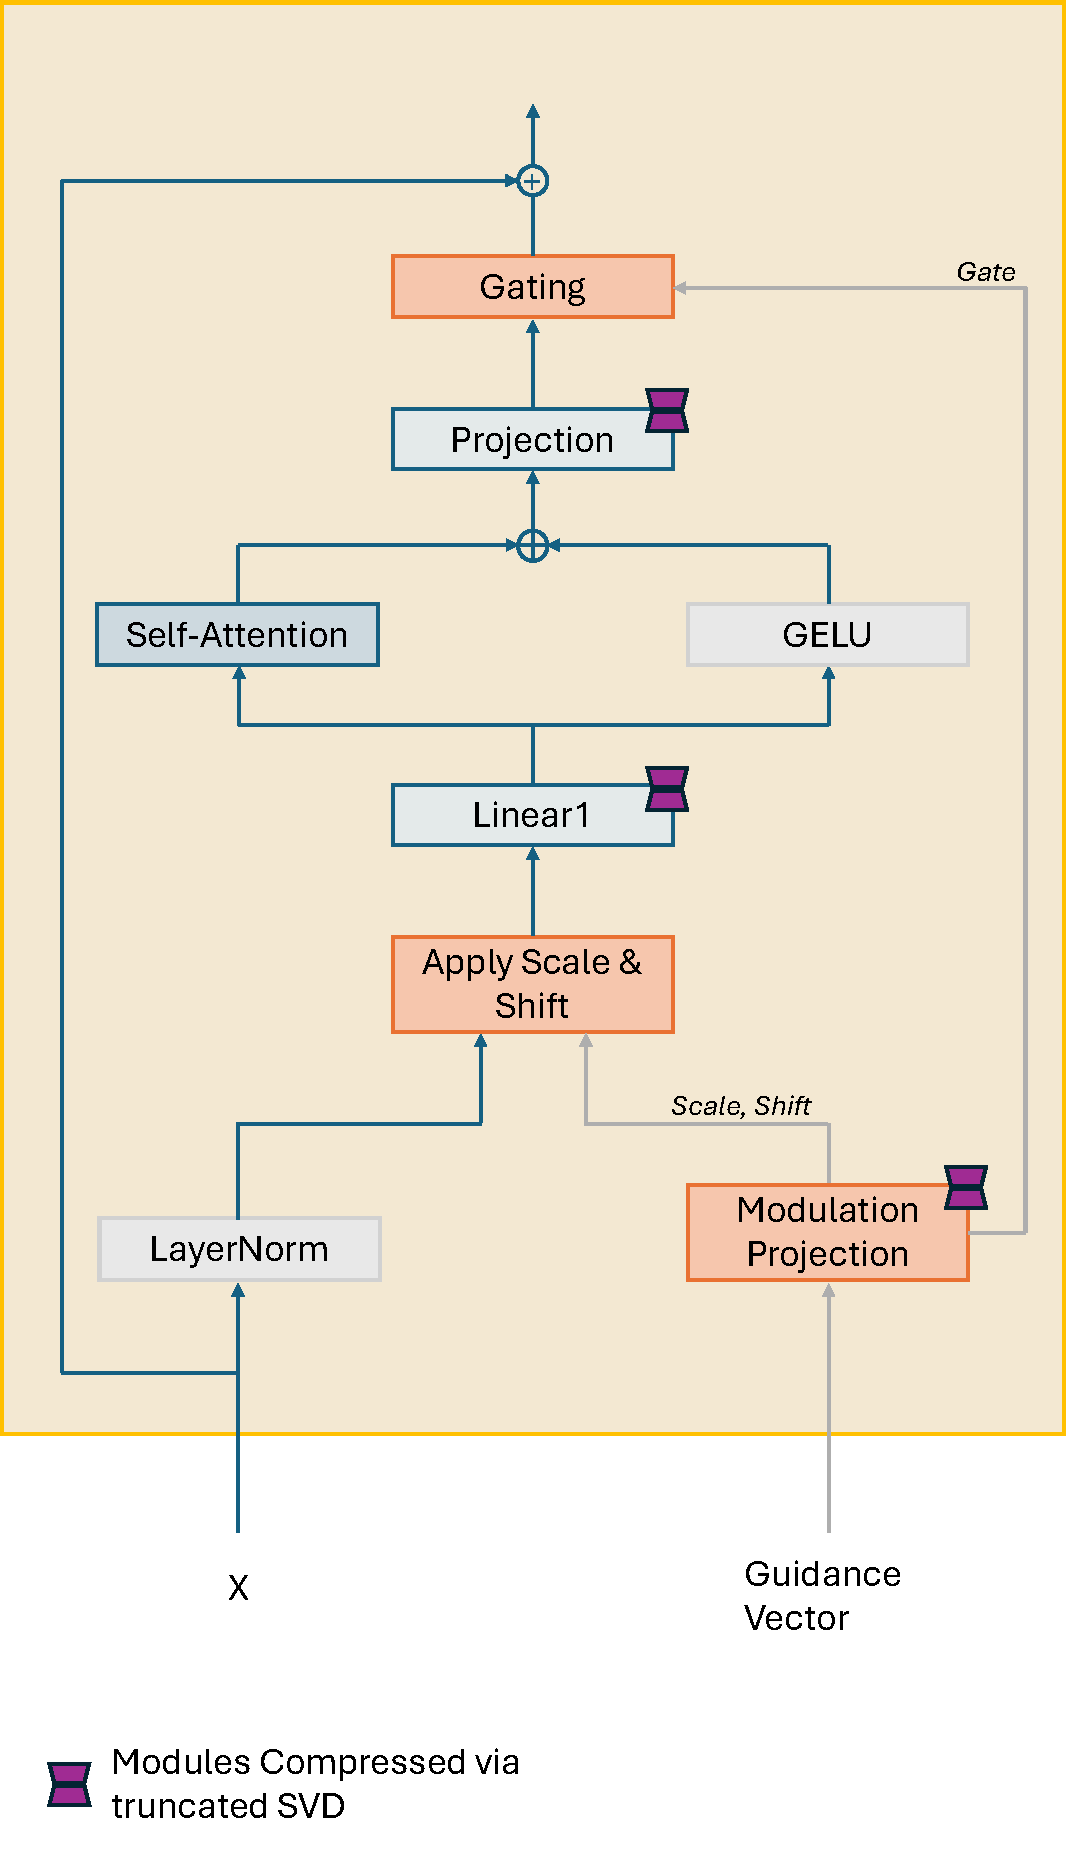
\includegraphics[width=0.4\textwidth]{images/Background/Flux/SingleBlockCompression.pdf}
	\caption[SVD Compressed Components of a FLUX.1 {[dev]} Single-Stream Block]{Architectural overview of the single-stream block components targeted for \gls{SVD}-based compression in FLUX.1 {[dev]}.}
	\label{fig:ArchSingleBlockComp}
\end{figure}


\begin{figure}[H]
	\centering
	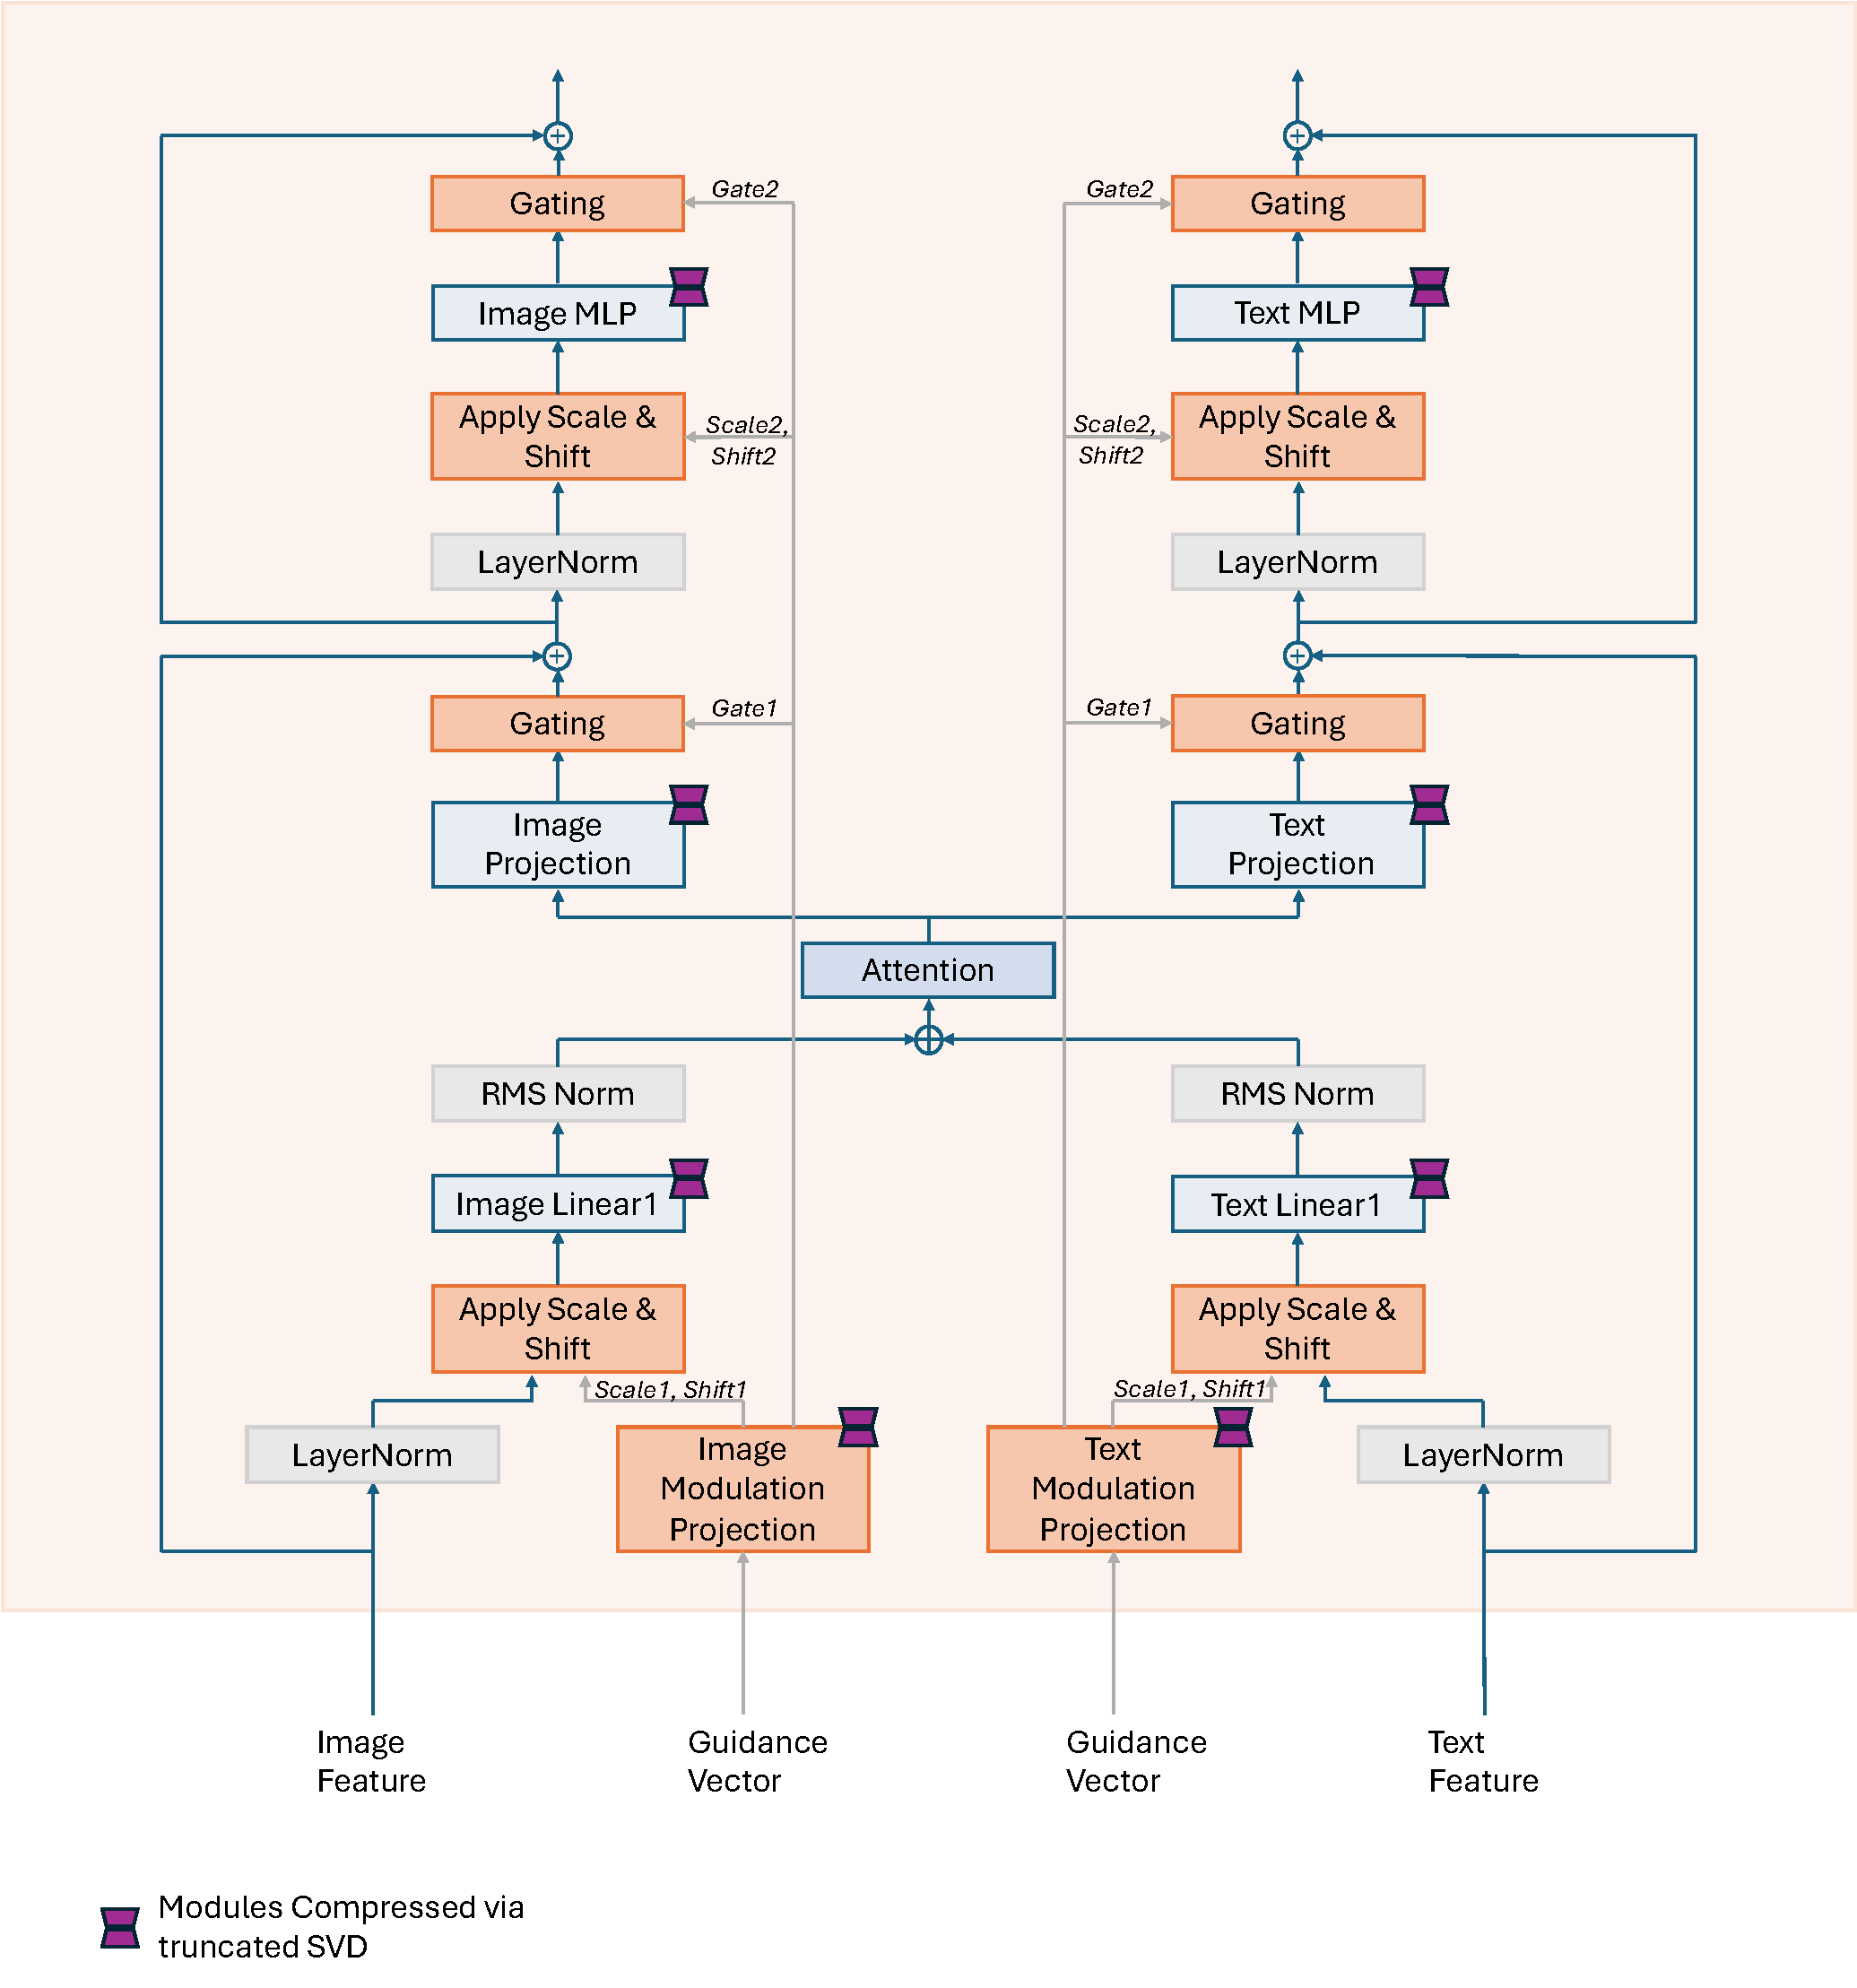
\includegraphics[width=0.8\textwidth]{images/Background/Flux/DoubleBlockCompression.pdf}
	\caption[SVD Compressed Components of a FLUX.1 {[dev]} Double-Stream Block]{Architectural overview of the double-stream block components targeted for \gls{SVD}-based compression in FLUX.1 {[dev]}.}
	\label{fig:ArchDoubleBlockComp}
\end{figure}


\begin{table}[H]
	\centering
	\caption[FLUX.1 {[dev]} Fine-Tuning Hyperparameters]{Configuration details for the compressed model retraining, including optimizer settings and flow matching specific parameters. These parameters represent the configuration setup for the training using the git repository \cite{kohya_ss_sd_scripts_2024}.}
	\label{tab:flux_training_config}
	\begin{tabular}{l l}
		\toprule
		\textbf{Hyperparameter} & \textbf{Value} \\
		\midrule
		\multicolumn{2}{l}{\textit{\textbf{Optimization \& Scheduler}}} \\
		Optimizer Type & Adafactor \\
		Optimizer Arguments & \small{relative\_step=False, scale\_parameter=False, warmup\_init=False} \\
		Learning Rate & $1.8 \times 10^{-6}$ \\
		LR Scheduler & constant\_with\_warmup \\
		LR Warmup Steps & 4240 \\
		Gradient Accumulation & 4 \\
		Batch Size & 1 \\
		\midrule
		\multicolumn{2}{l}{\textit{\textbf{Model Precision \& Hardware}}} \\
		Mixed Precision & bf16 \\
		Weight Precision (Base) & fp8 \\
		Full bfloat16 Training & True \\
		Gradient Checkpointing & True \\
		SDPA (Scaled Dot Product Attn) & True \\
		GPU & 1 $\times$ H200 \\
		\midrule
		\multicolumn{2}{l}{\textit{\textbf{Flow Matching \& Loss Settings}}} \\
		Discrete Flow Shift & 3 \\
		Timestep Sampling & sigmoid \\
		Max Timestep & 1000 \\
		Loss Type & L2 \\
		Huber Parameter ($c$) & 0.1 \\
		Huber Schedule & snr \\
		Model Prediction Type & raw \\
		Guidance Scale & 1.0 \\
		Sample Sampler & euler\_a \\
		\midrule
		\multicolumn{2}{l}{\textit{\textbf{Architecture \& Data Settings}}} \\
		T5 Max Token Length & 512 \\
		Clip Skip & 1 \\
		Apply T5 Attn Mask & True \\
		Data Loader Workers & 6 \\
		Seed & 42 \\
		Training Dataset & LAION-FLUX.1 {[dev]}\\
		Size Training Dataset & 190 000 \\
		\bottomrule
	\end{tabular}
\end{table}


\section{Qualitative Block Importance Analysis}
\label{appx:FluxBlockImportanceAnalysis}
Fig. \ref{fig:AppxBlockAnalysisRemovalDouble} and Fig. \ref{fig:AppxBlockAnalysisRemovalSingle} present the complete set of qualitative examples of a generated images when one complete double- or single-stream block is pruned similar to the analysis in Sec. \ref{sec:QualitativeBlockAnalysisFlux}. 

Fig. \ref{fig:AppxBlockAnalysisCompressionDouble} and Fig. \ref{fig:AppxBlockAnalysisCompressionSingle} present qualitative examples of a generated images when one complete double- or single-stream block is compressed via truncated \gls{SVD}. 

Furthermore, Fig. \ref{fig:AppxBlockRanking} displays the block ranking for the uncompressed FLUX.1 [dev] based on the parameter-weighted \gls{CMMD} values.


\begin{figure}[H]
	\centering
	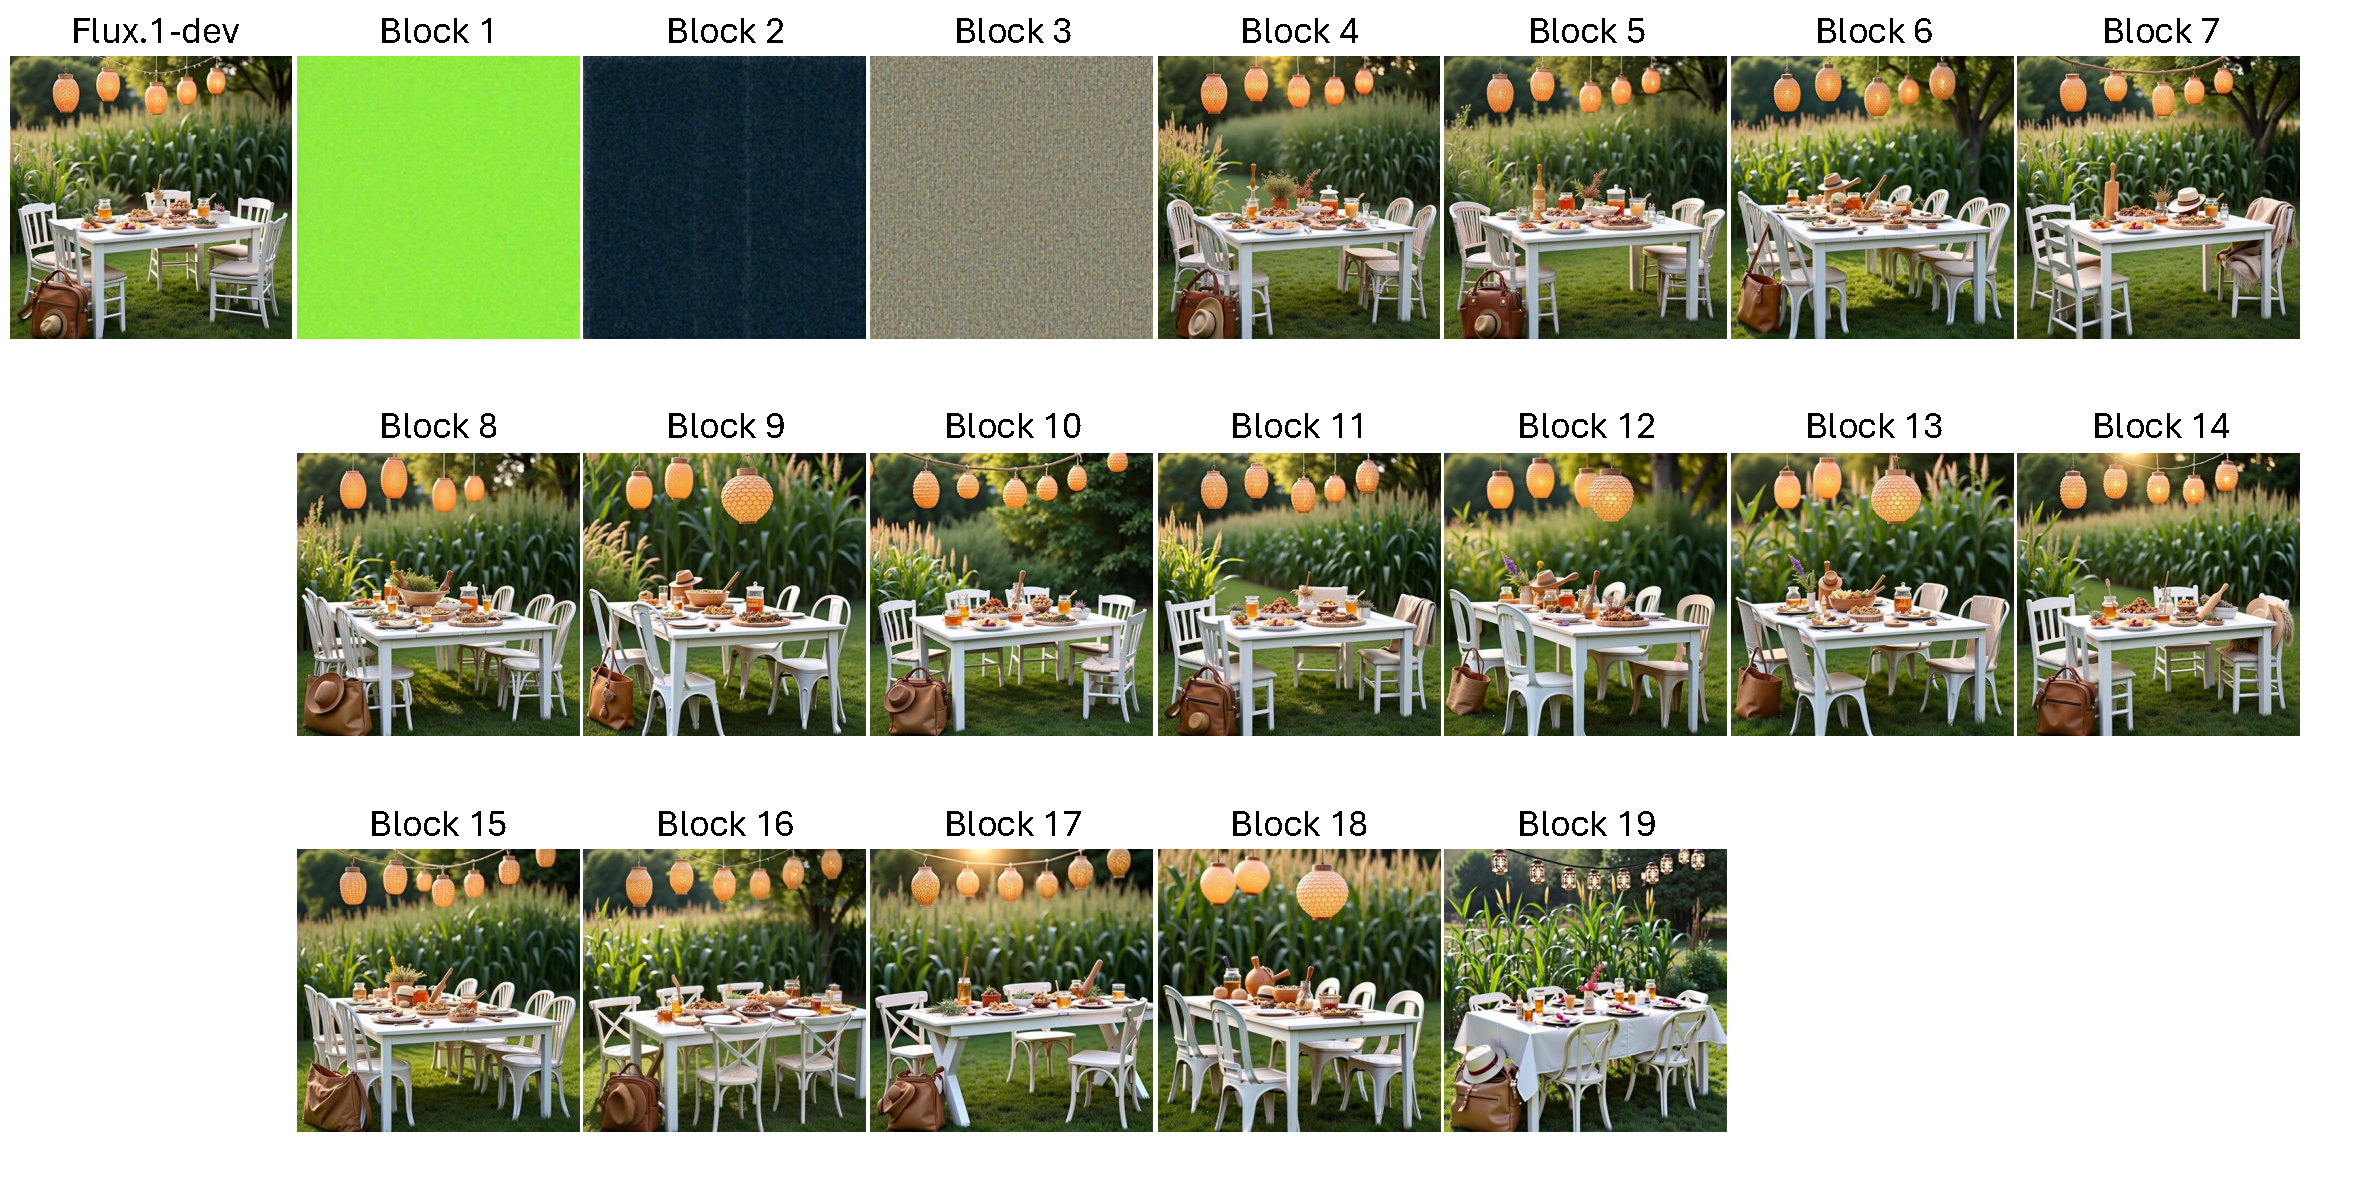
\includegraphics[width=\textwidth]{images/Experimente/Flux/Block_Analysis/BlockRemovalDouble.pdf}
	\caption[Qualitative Double-Stream Block Importance Analysis of FLUX.1 {[dev]}: Block Removal]{Qualitative comparison of the impact of complete removal of individual double-stream blocks in FLUX.1 {[dev]}.}
	\label{fig:AppxBlockAnalysisRemovalDouble}
\end{figure}

\begin{figure}[H]
	\centering
	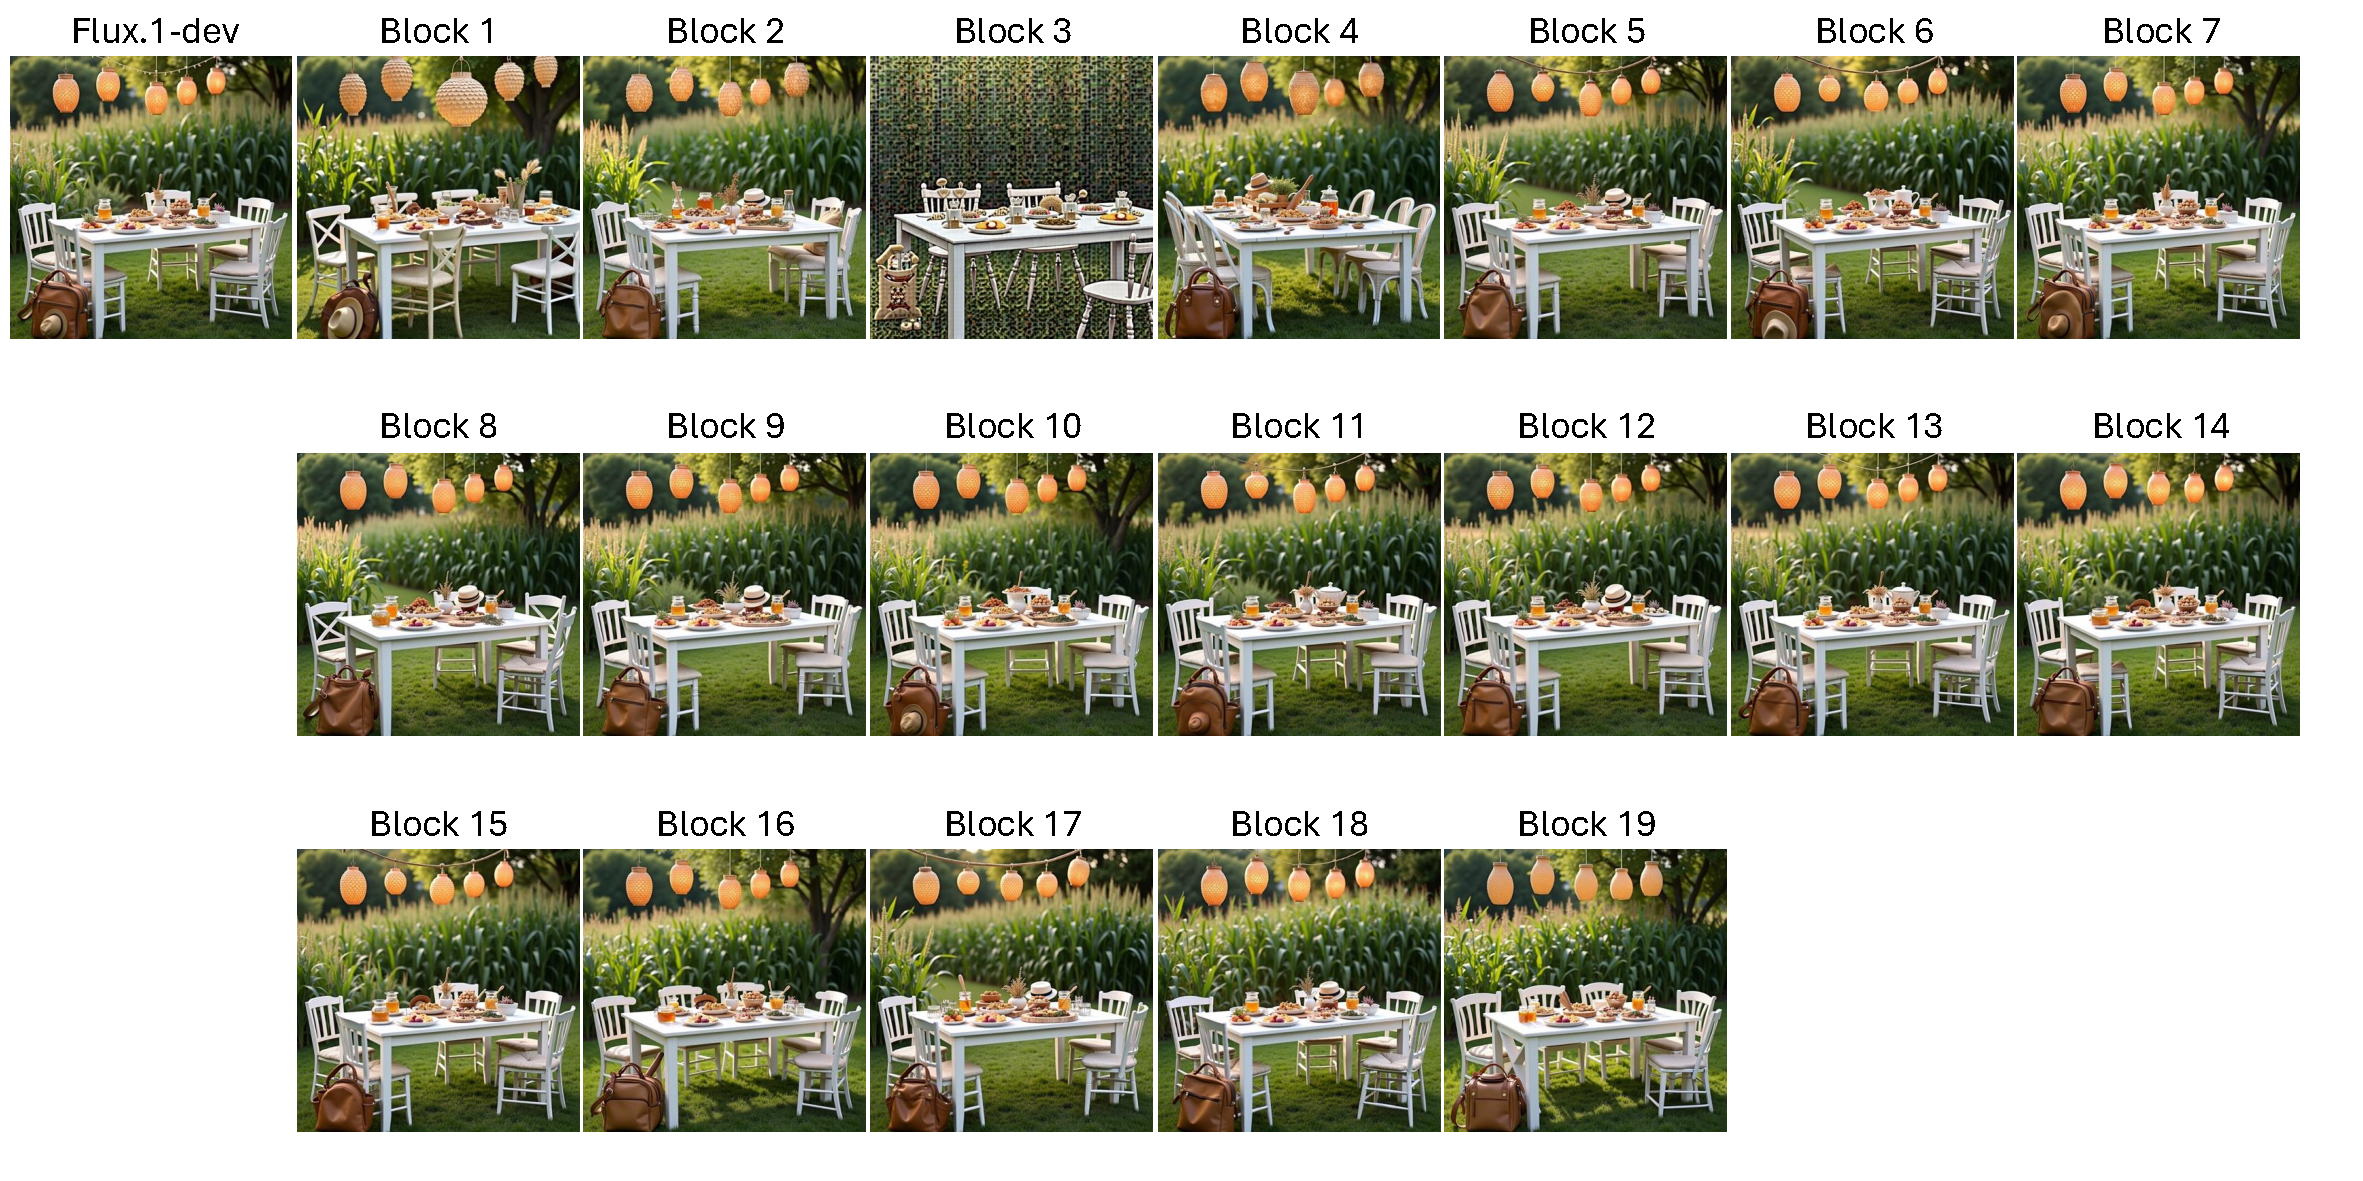
\includegraphics[width=\textwidth]{images/Experimente/Flux/Block_Analysis/BlockCompressionDouble.pdf}
	\caption[Qualitative Double-Stream Block Importance Analysis of FLUX.1 {[dev]}: Block Compression]{Qualitative comparison of the impact of 60\% \gls{SVD}-based compression of individual double-stream blocks in FLUX.1 {[dev]}.}
	\label{fig:AppxBlockAnalysisCompressionDouble}
\end{figure}


\begin{figure}[H]
	\centering
	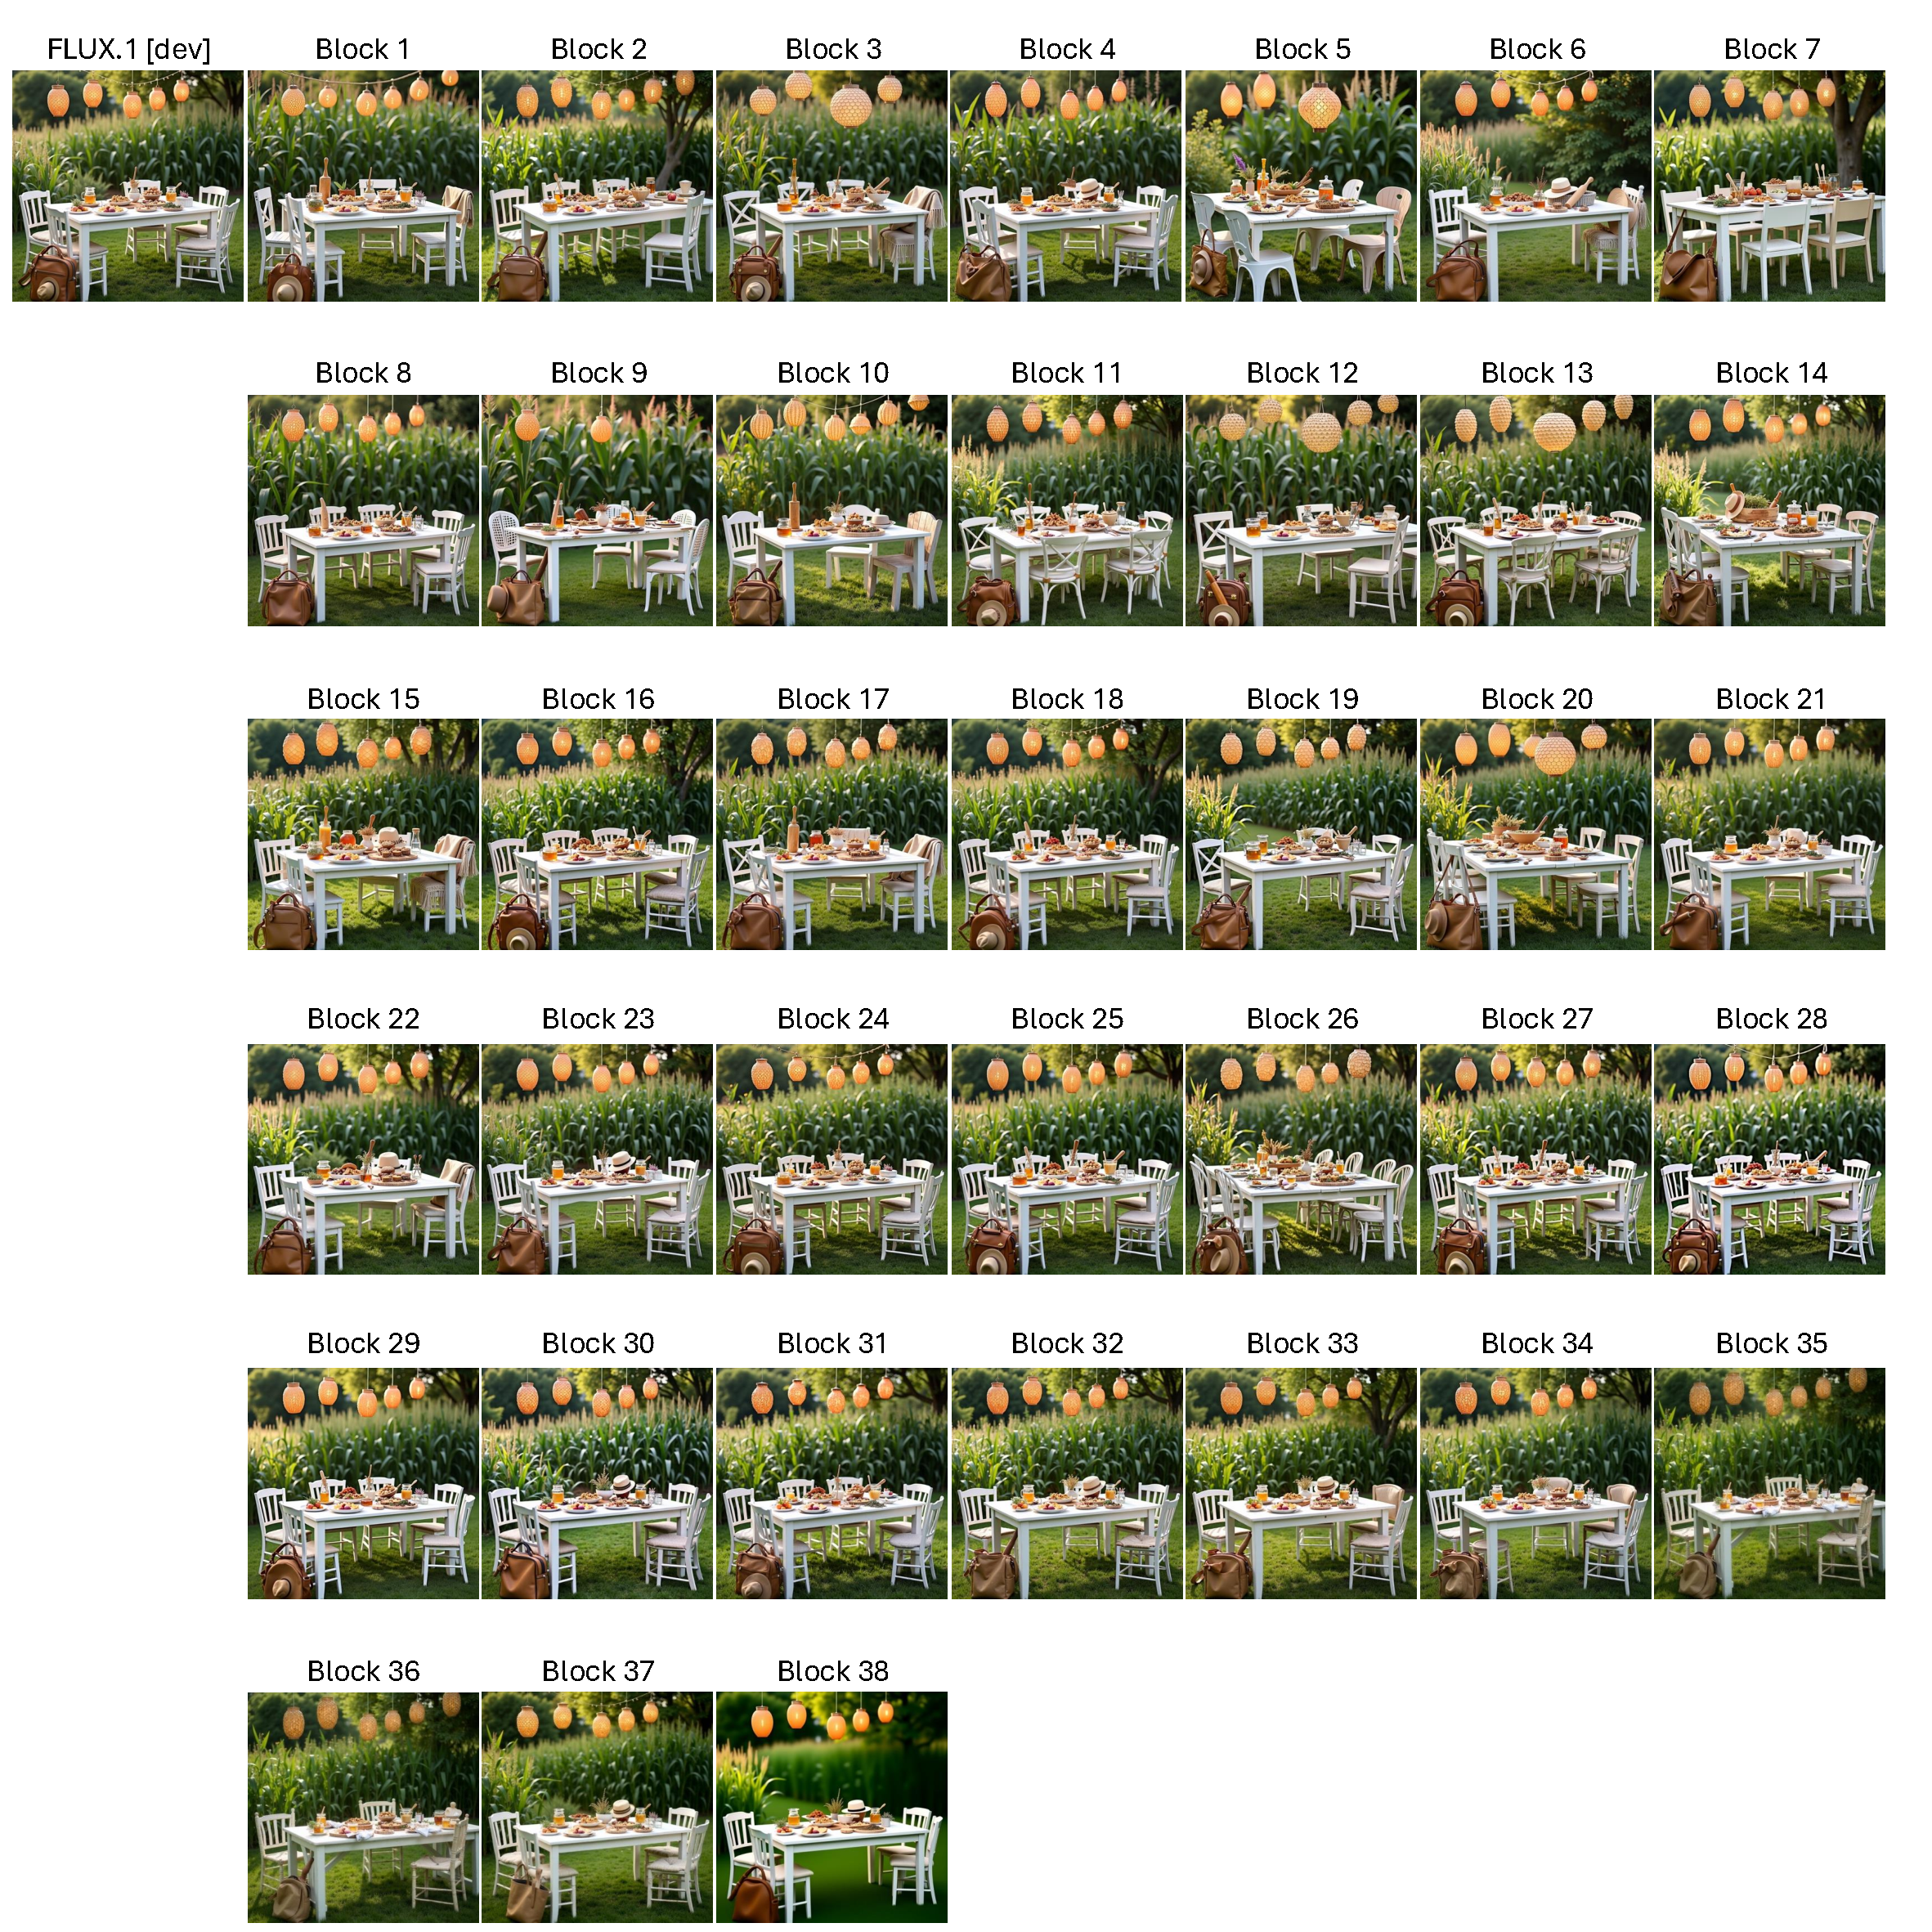
\includegraphics[width=\textwidth]{images/Experimente/Flux/Block_Analysis/BlockRemovalSingle.pdf}
	\caption[Qualitative Single-Stream Block Importance Analysis of FLUX.1 {[dev]}: Block Removal]{Qualitative comparison of the impact of complete removal of individual single-stream blocks in FLUX.1 {[dev]}.}
	\label{fig:AppxBlockAnalysisRemovalSingle}
\end{figure}



\begin{figure}[H]
	\centering
	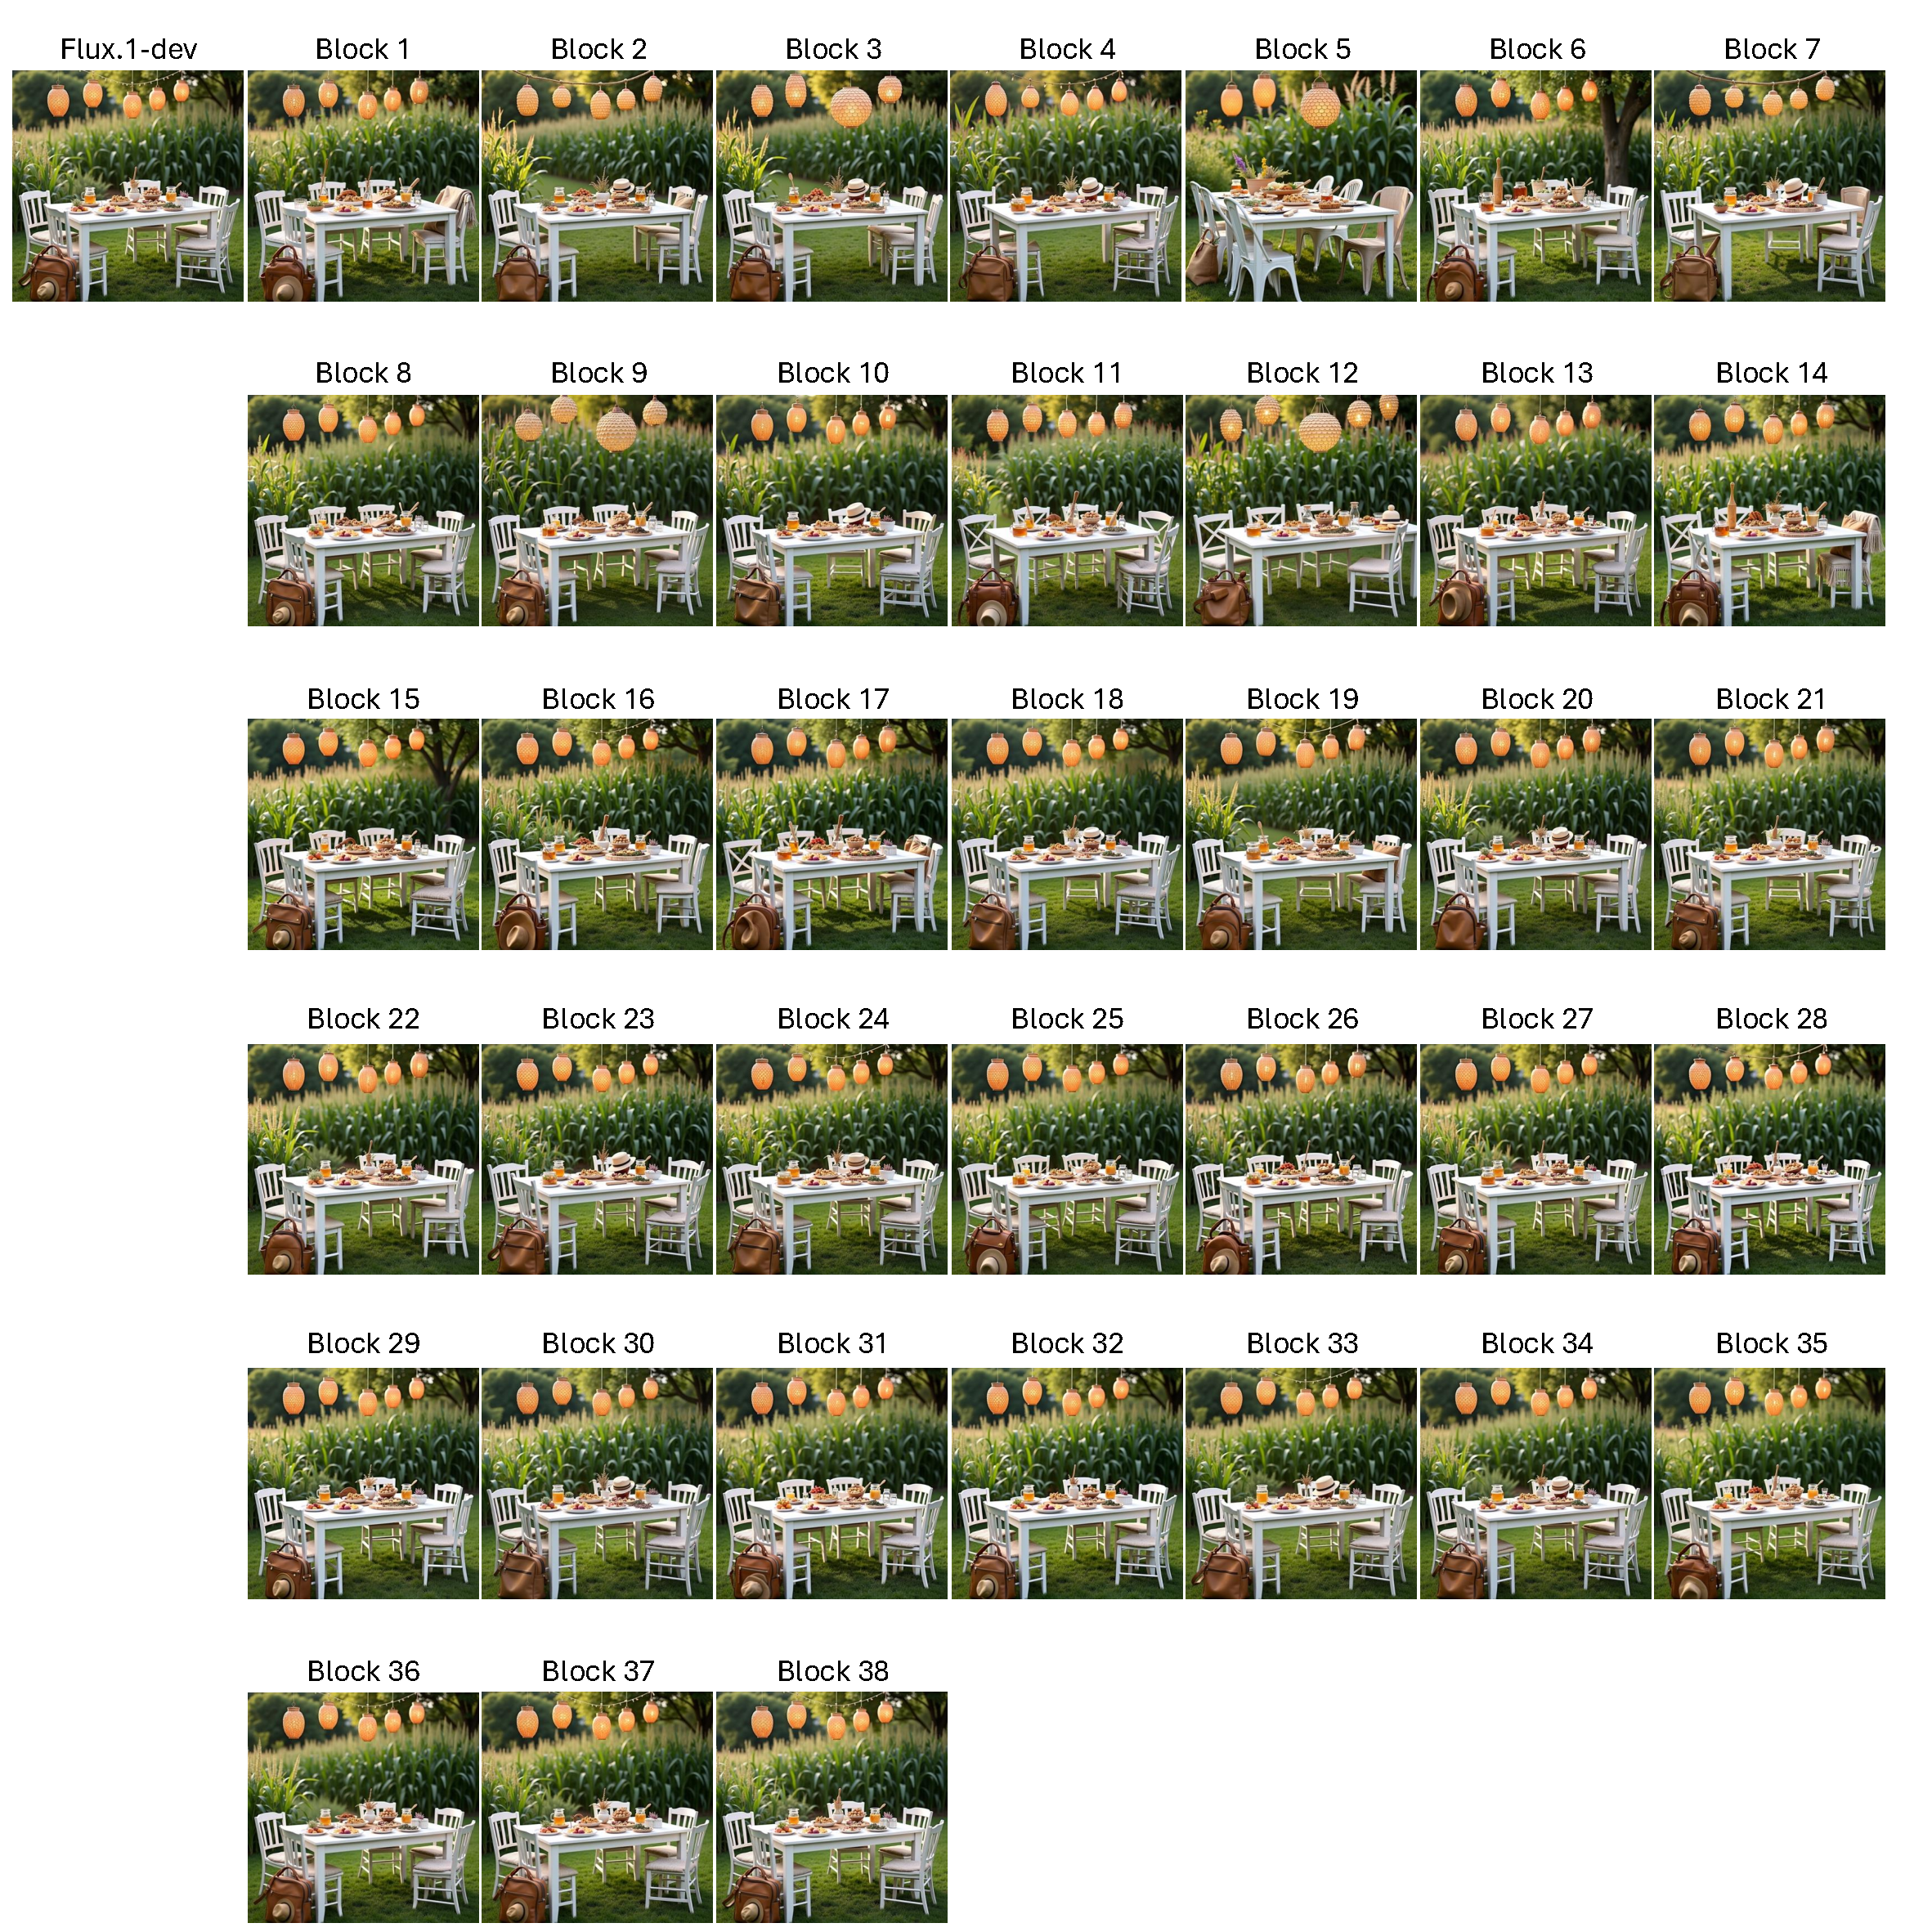
\includegraphics[width=\textwidth]{images/Experimente/Flux/Block_Analysis/BlockCompressionSingle.pdf}
	\caption[Qualitative Single-Stream Block Importance Analysis of FLUX.1 {[dev]}: Block Compression]{Qualitative comparison of the impact of 60\% \gls{SVD}-based compression of individual single-stream blocks in FLUX.1 {[dev]}.}
	\label{fig:AppxBlockAnalysisCompressionSingle}
\end{figure}



\begin{figure}[H]
	\centering
	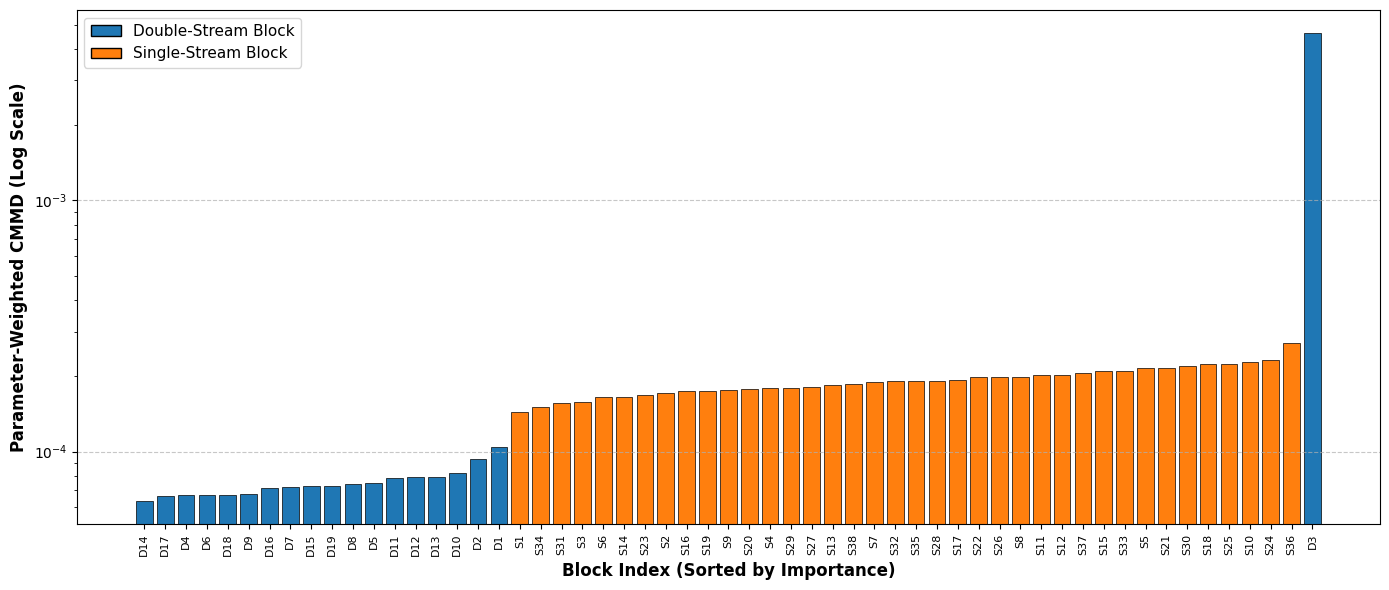
\includegraphics[width=\textwidth]{images/Experimente/Flux/Block_Analysis/weightedCMMD.png}
	\caption[Block Ranking FLUX.1 {[dev]}]{Block ranking for FLUX.1 {[dev]} based on parameter-weighted \gls{CMMD} value obtained by compressing each block individually ($c_\text{fixed}=60\%$).}
	\label{fig:AppxBlockRanking}
\end{figure}


\newpage
\section{Training-Free Model Compression}
This section provides the technical settings for the training-free experiments (Sec. \ref{sec:trainingFreeCompression}) using complete block removal (Tab. \ref{tab:TrainingFreeMethodsRemoval}) and \gls{SVD}-based compression (Tab. \ref{tab:TrainingFreeMethodsSVD}). Additionally, it presents example images for models compressed to 90\% and 70\% (Figs. \ref{fig:Examples_TrainingFree90} - \ref{fig:Examples_TrainingFree70}).


\begin{table}[H]
	\centering
	\caption[Training-Free Compression: \gls{SVD} Compression Details]{Details about importance-aware rank-adaptive progressive pruning schedule applied for \gls{SVD} based-compression in training-free setting.}
	\label{tab:TrainingFreeMethodsSVD}
	\begin{tabular}{@{}lccc@{}}
		\toprule
		\textbf{Model Size} & \textbf{Modified Blocks} & \textbf{Base Compression Ratio}  & \textbf{Linear Decay Rate $x$}  \\ \midrule
		90\% & 30 & 25\% & 0.0083 \\
		80\% & 30 & 50\% & 0.0166\\
		70\% & 30 & 75\% & 0.0249\\
		\bottomrule
	\end{tabular}
\end{table}

\begin{table}[H]
	\centering
	\caption[Training-Free Compression: Complete Block Removal Details]{Details about complete block removal scheme in training-free setting.}
	\label{tab:TrainingFreeMethodsRemoval}
	\begin{tabular}{@{}lccc@{}}
		\toprule
		\textbf{Model Size} & \textbf{No. Removed Blocks} & \textbf{Removed Double Blocks}   \\ \midrule
		90\% & 3 & 14, 17, 6\\
		80\% & 7 & 14, 17, 4, 6, 18, 9, 16\\
		70\% & 10 & 14, 17, 4, 6, 18, 9, 16, 7, 15, 19\\
		\bottomrule
	\end{tabular}
\end{table}


\begin{figure}[H]
	\centering
	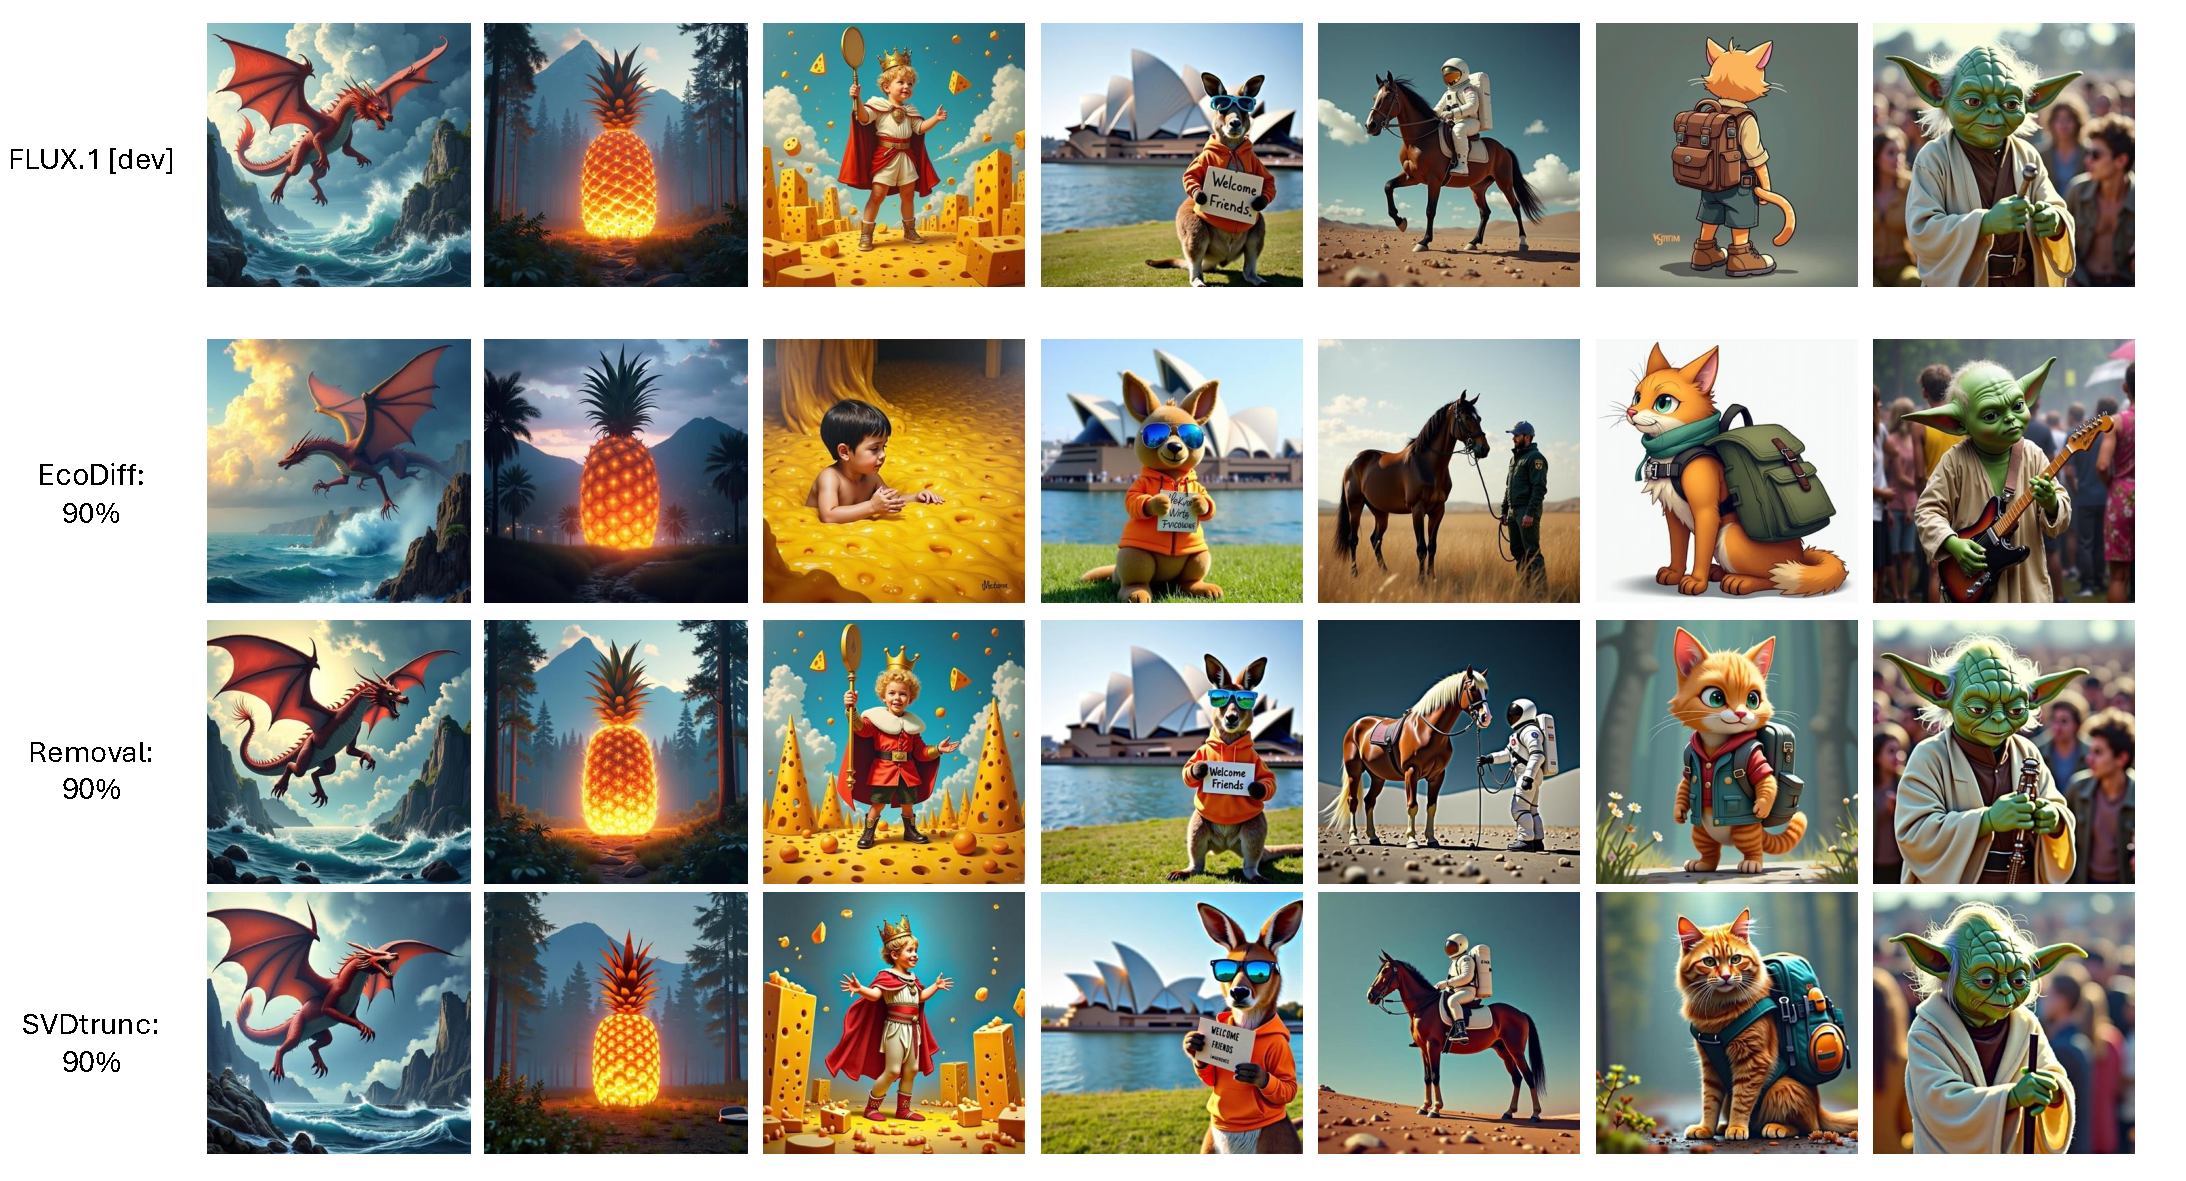
\includegraphics[width=\textwidth]{images/Experimente/Flux/TrainingFree_paper/TrainingFreeAppendix_model90.pdf}
	\caption[Qualitative Examples: Training-Free Model Compression (90\% Model)]{Qualitative comparison of example images generated by models compressed to 90\% using EcoDiff, complete block removal, and truncated \gls{SVD} compression without fine-tuning.}
	\label{fig:Examples_TrainingFree90}
\end{figure}

\begin{figure}[H]
	\centering
	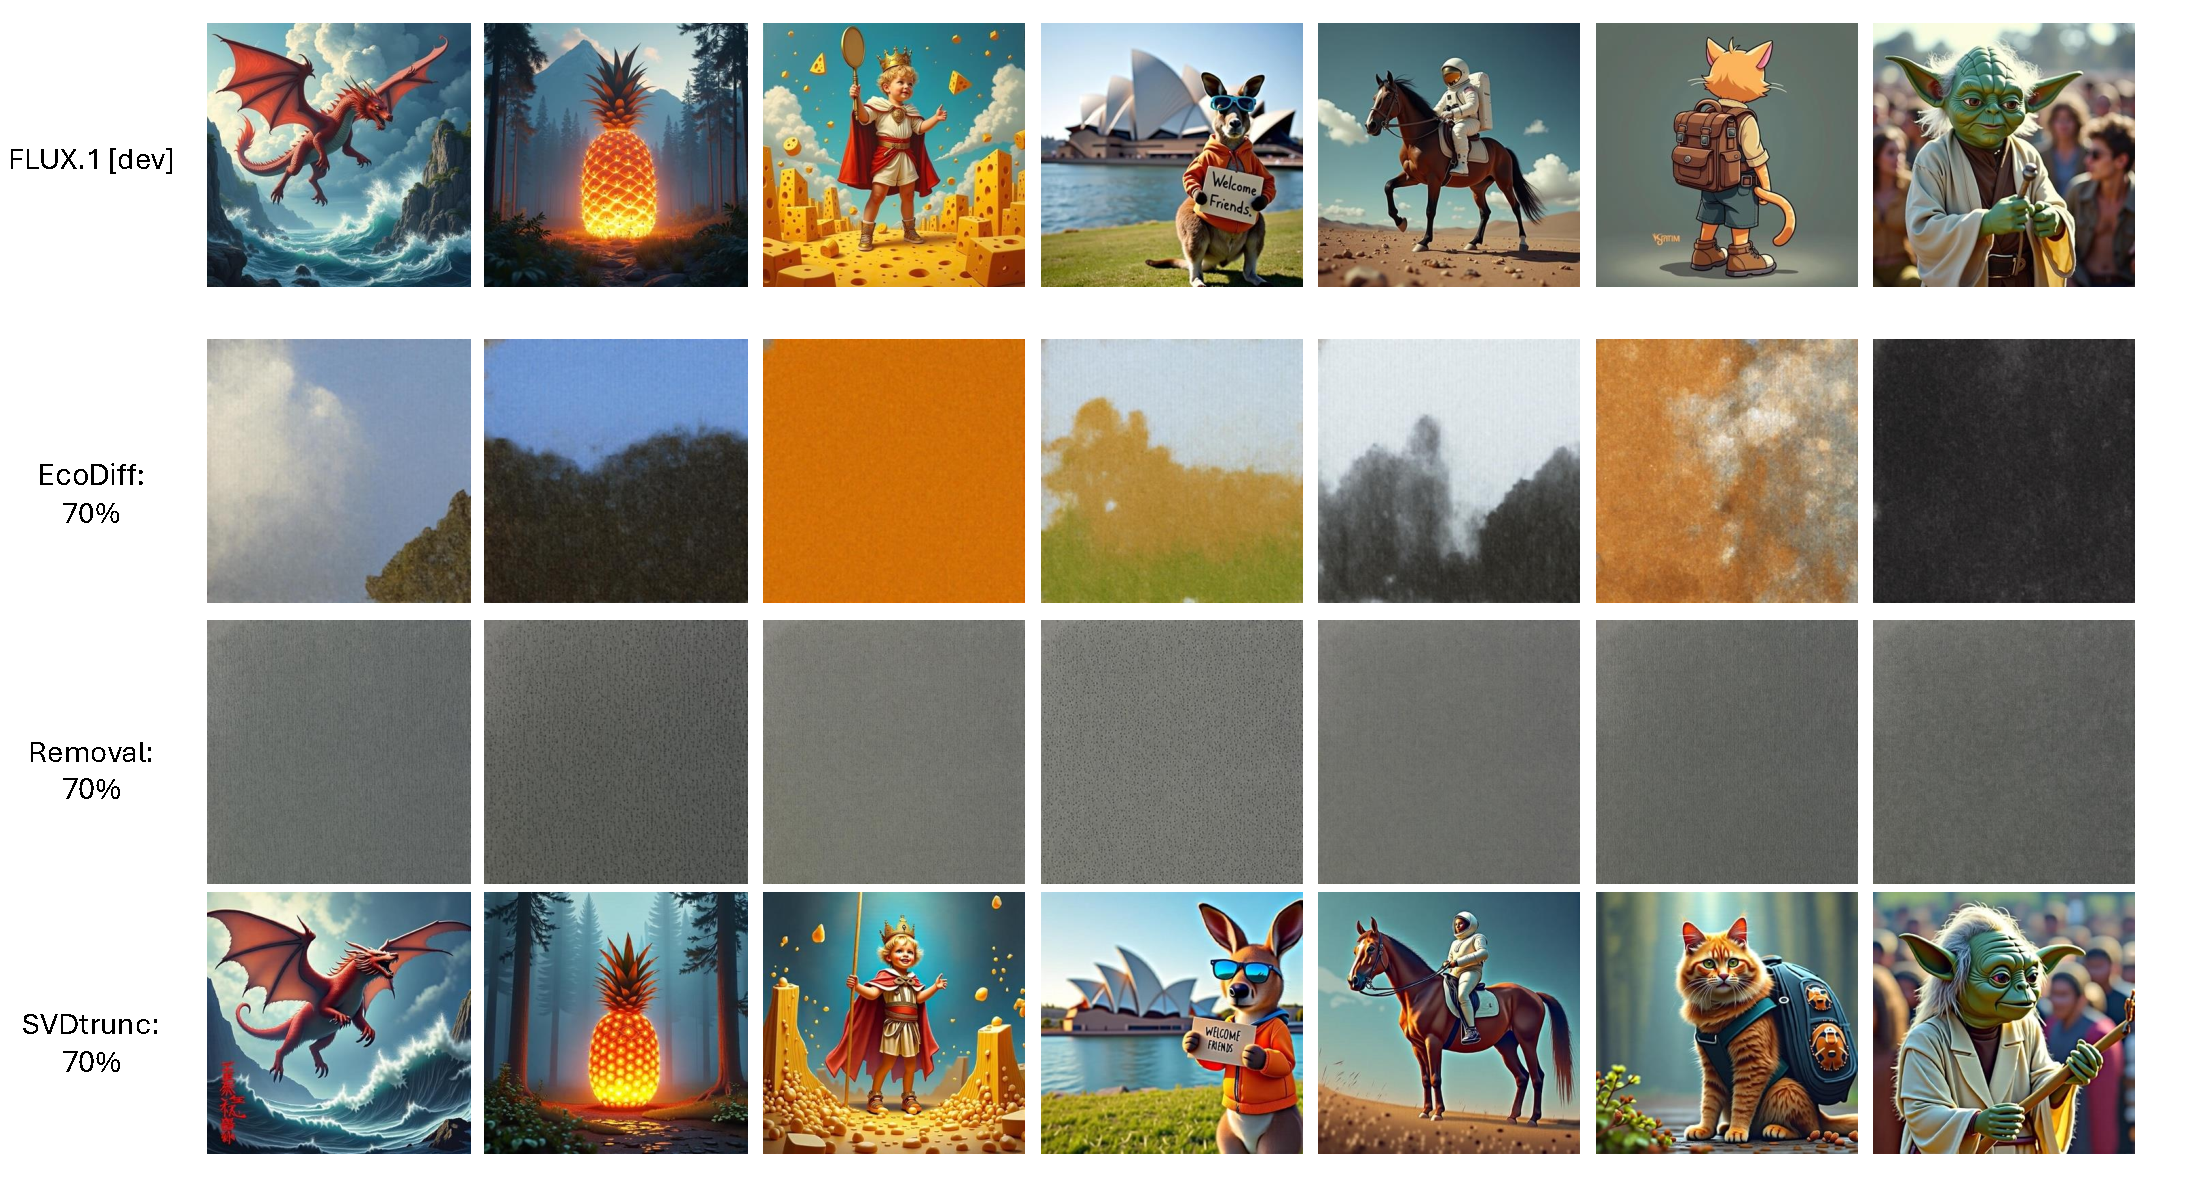
\includegraphics[width=\textwidth]{images/Experimente/Flux/TrainingFree_paper/TrainingFreeAppendix_model70.pdf}
	\caption[Qualitative Examples: Training-Free Model Compression (70\% Model)]{Qualitative comparison of example images generated by models compressed to 70\% using EcoDiff, complete block removal, and truncated \gls{SVD} compression without fine-tuning.}
	\label{fig:Examples_TrainingFree70}
\end{figure}

\section{Preliminary Experiments: Block Selection and Compression Schedule}

\subsection{Block Selection}
\label{sec:FluxBlockImportanceAnalysisAppendix}
Tab. \ref{tab:Random_vs_metric_Selection} summarizes the experimental settings for the uniform selection process presented in Section \ref{sec:FluxBlockImportanceAnalysis}. Tab. \ref{tab:RandomBlockSelectionDetails} presents details of the compression setup for the random block selection strategy. Furthermore, this subsection presents qualitative example images (Figs. \ref{fig:FluxBlockSelection_68}--\ref{fig:FluxBlockSelection_43}) generated by FLUX.1 {[dev]} models at various compression stages. These images were obtained using random, uniform, and importance-aware block selection strategies.







\begin{table}[h]
	\centering
	\caption[Uniform Block Selection: Compression Details]{Overview of compression and fine-tuning details for the uniform block selection experiment.}
	\label{tab:Random_vs_metric_Selection}
	\begin{tabular}{c c  c c}
		\toprule
		\textbf{Iteration} & \textbf{Model Size (\%)} & \textbf{Training Steps} \\
	&& \textbf{per Iteration} \\
		\midrule
		1 & 68\%    & 40k \\ % Beispielwerte
		2 & 57\%   & 20k \\
		3 & 49\%   & 20k \\
		4 & 43\%  & 20k \\
		\bottomrule
	\end{tabular}
\end{table}



\begin{table}[H]
	\centering
	\caption[Random Block Selection: Compression Details]{Overview of the experimental settings for the FLUX.1 [dev] compression where blocks were \textbf{randomly} selected, detailing how the removed parameters are distributed across varying numbers of blocks. For readability, the linear decay rate $x$ is scaled by 1000.}
	\label{tab:RandomBlockSelectionDetails}
	\begin{tabular}{cccccc}
		\toprule
		\textbf{Iteration} &\textbf{Model Size} & \textbf{Training Steps} & \textbf{Number of} & \textbf{Base Compression} & \textbf{Linear Decay}\\
		&&&\textbf{Modified Blocks}&\textbf{Ratio}& \textbf{Rate} $x$\\
		\midrule
		
		1 &  68\%&  40,000 & 49 & 0.6 & 9.4 \\
		
	
		
		
		2 & 57\% & 20,000 &  30 & 0.5 & 11.2 \\
		

		
		3 & 49\% & 20,000 &  30 & 0.4  & 9.5 \\
		
	
		
		4& 43\% &  20,000 & 30 & 0.4  & 11.5 \\
		
		
		
		\bottomrule
	\end{tabular}
\end{table}


\begin{figure}[H]
	\centering
	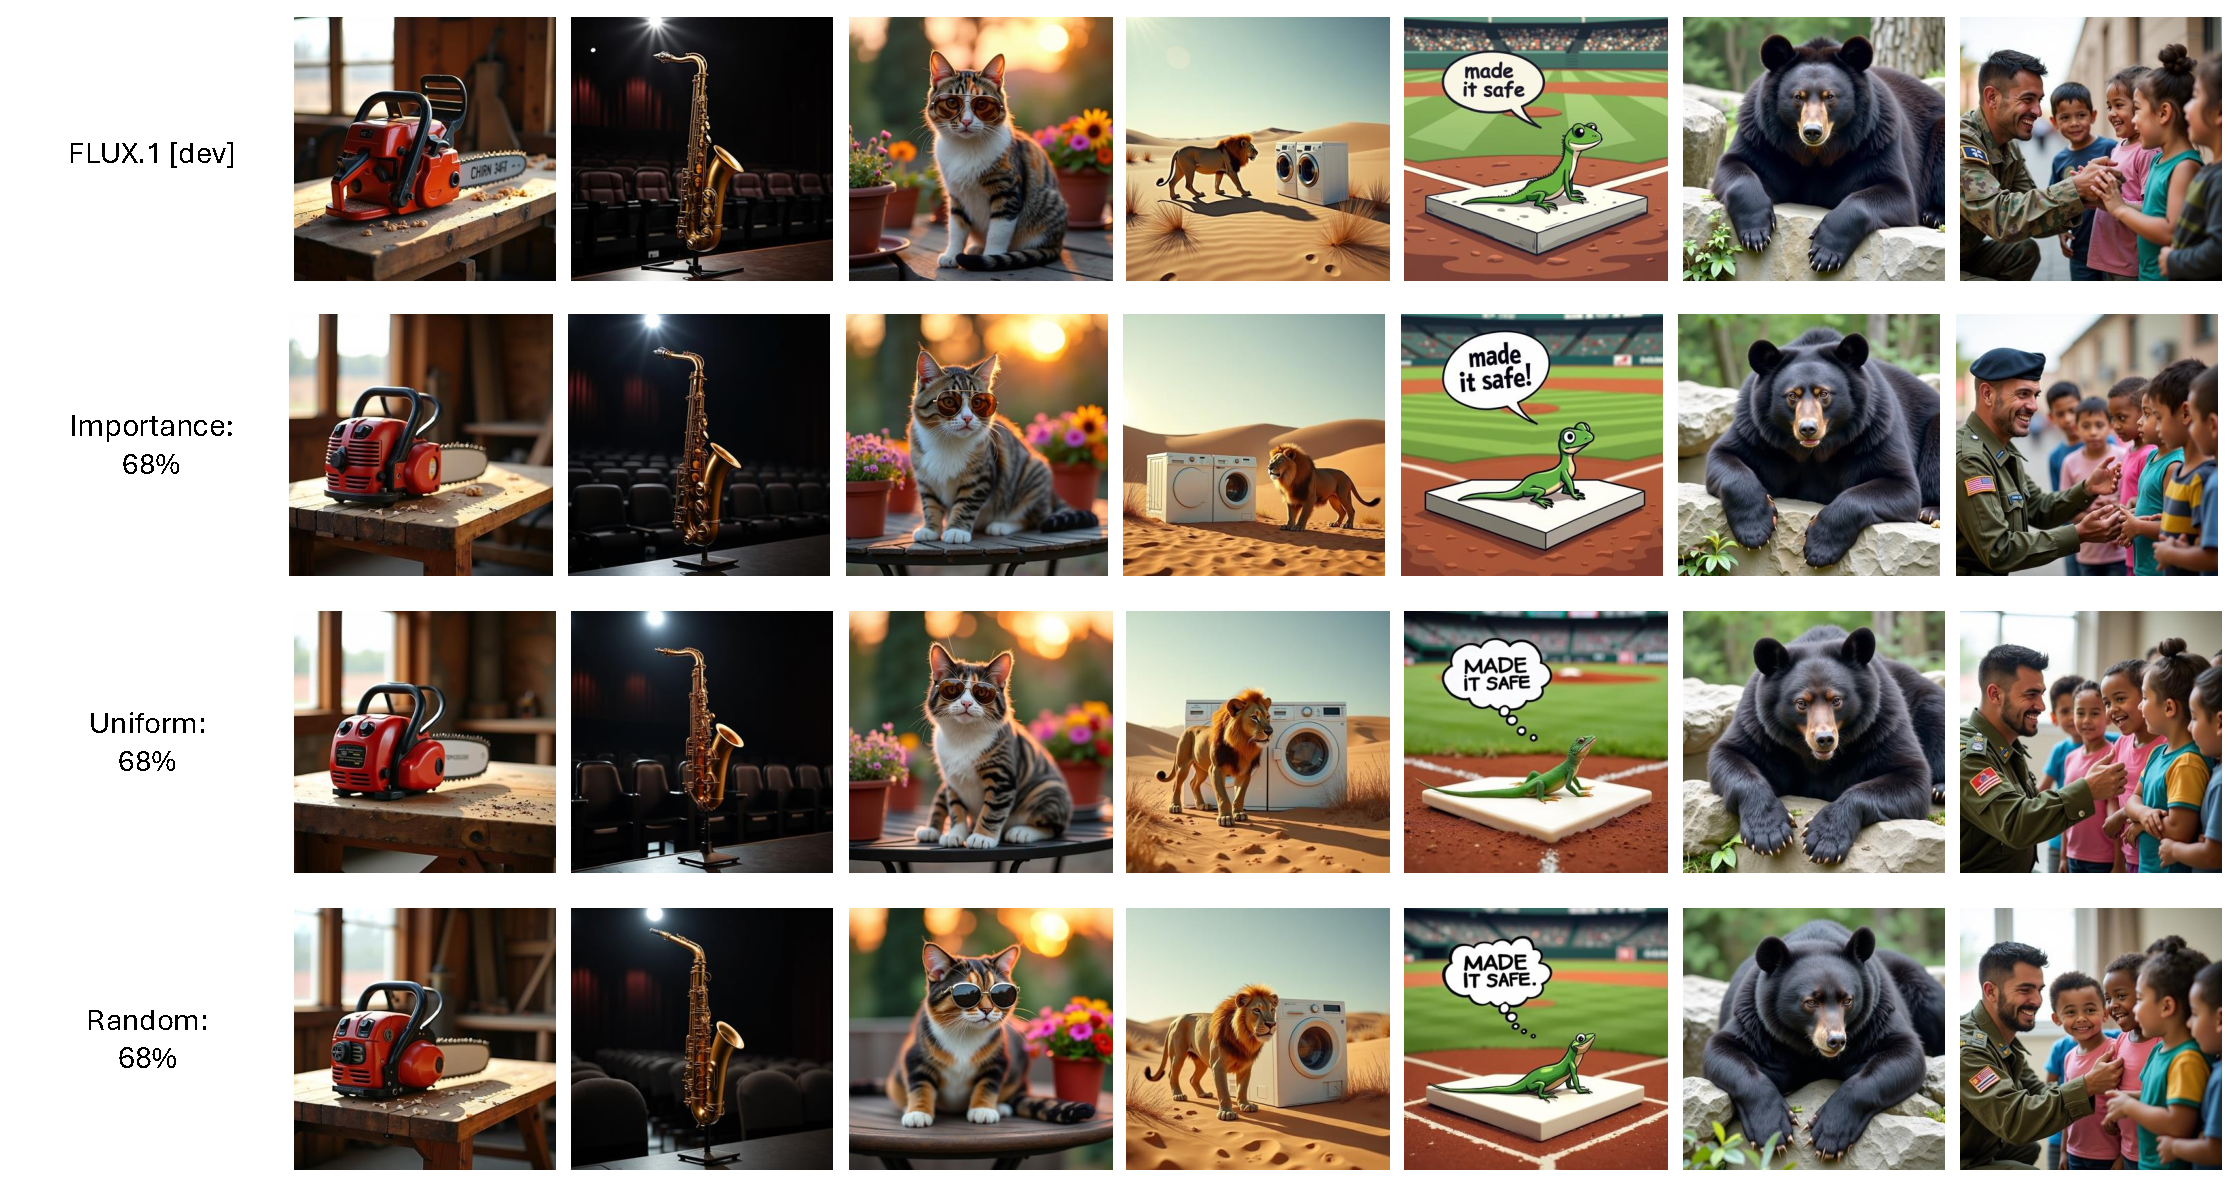
\includegraphics[width=\textwidth]{images/Experimente/Flux/BlockSelection/Random_vs_Importance_Block_Selection_Appendix_model_68.pdf}
	\caption[Qualitative Examples: Importance, Uniform, and Random Block Selection (68\% Model)]{Qualitative comparison of example images generated by models compressed to 68\% obtained by random, uniform, and importance-based block selection.}
	\label{fig:FluxBlockSelection_68}
\end{figure}
\begin{figure}[H]
	\centering
	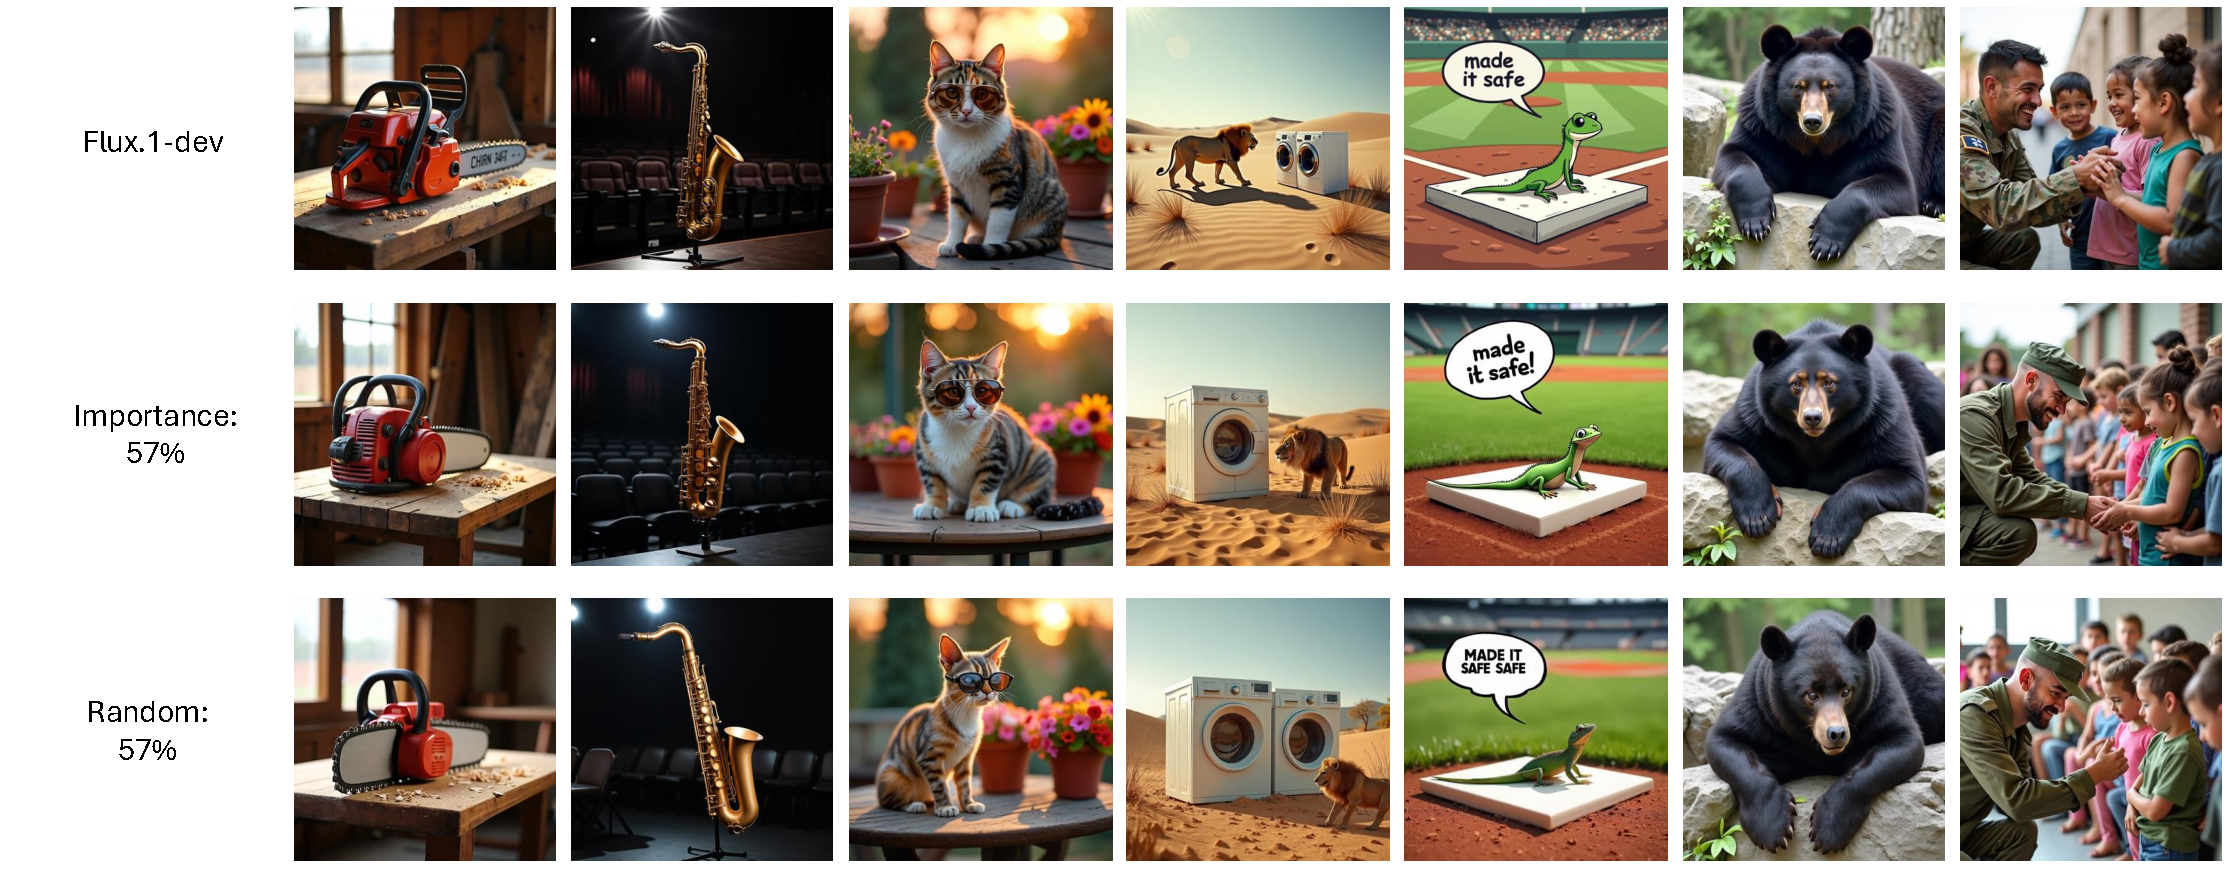
\includegraphics[width=\textwidth]{images/Experimente/Flux/BlockSelection/Random_vs_Importance_Block_Selection_Appendix_model_57.pdf}
	\caption[Qualitative Examples: Importance, Uniform, and Random Block Selection (57\% Model)]{Qualitative comparison of example images generated by models compressed to 57\% obtained by random, uniform, and importance-based block selection.}
	\label{fig:FluxBlockSelection_57}
\end{figure}
\begin{figure}[H]
	\centering
	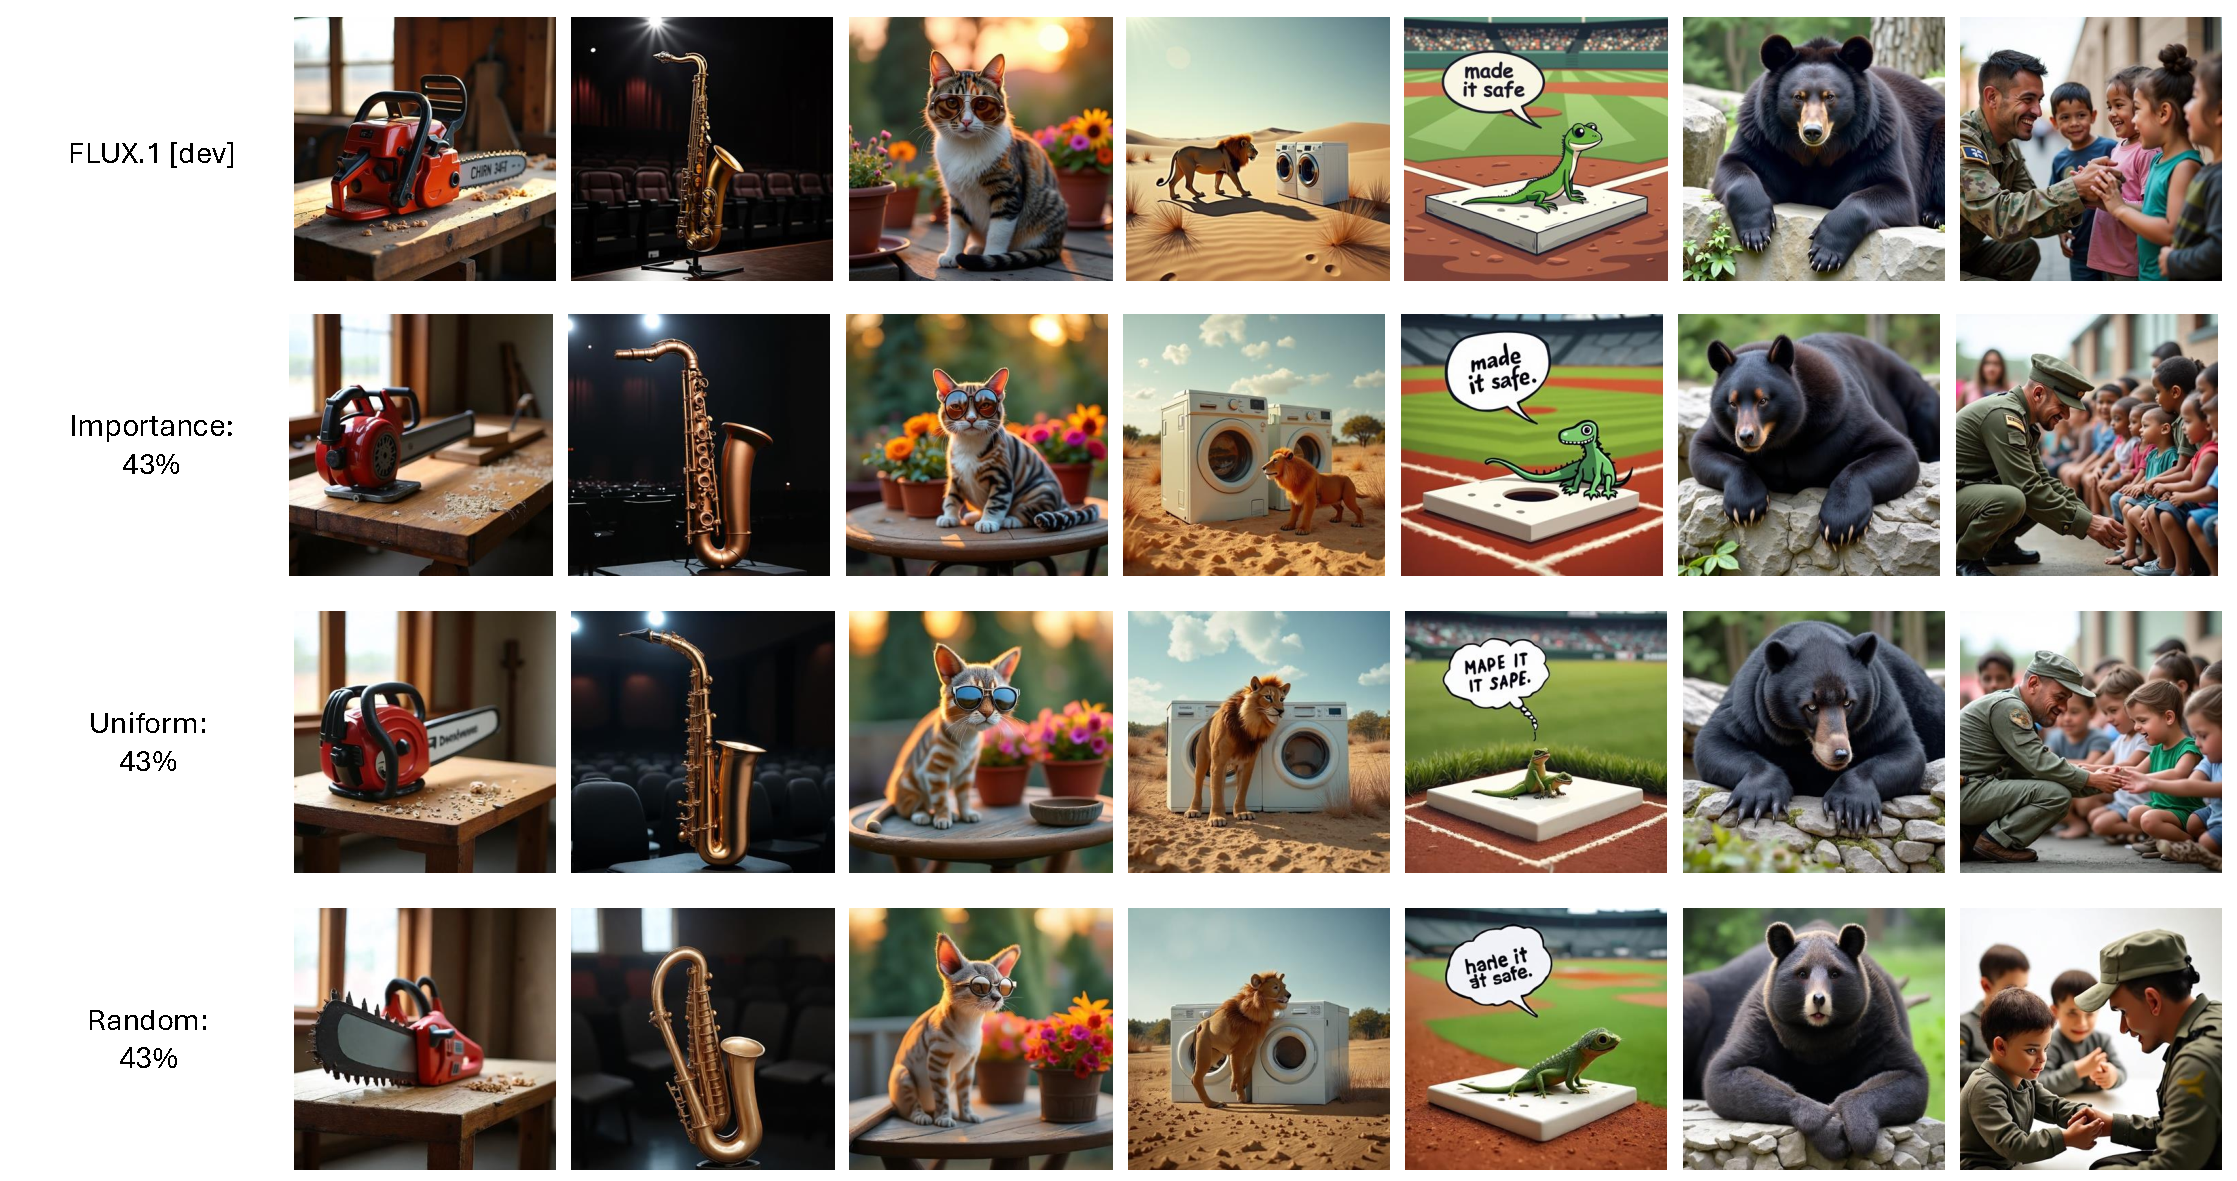
\includegraphics[width=\textwidth]{images/Experimente/Flux/BlockSelection/Random_vs_Importance_Block_Selection_Appendix_model_43.pdf}
	\caption[Qualitative Examples: Importance, Uniform, and Random Block Selection (43\% Model)]{Qualitative comparison of example images generated by models pruned to 43\% obtained by random, uniform, and importance-based block selection.}
	\label{fig:FluxBlockSelection_43}
\end{figure}

\newpage

\subsection{Sensitivity Analysis: Compression Breadth vs. Depth}
Tab. \ref{tab:compression_iterations} summarizes the experimental settings for the importance-aware rank-adaptive progressive compression schedule. These configurations explore how to optimally distribute the removed parameters across a varying number of Transformer blocks, as detailed in Section \ref{sec:FluxParameterRemovalDistribution}. As \textbf{30 Blocks} is identified as best setting, its detailed benchmark performances are presented in Tab. \ref{tab:hpsv_30blocks} - \ref{tab:dpg_30blocks}.


\begin{table}[H]
	\centering
	\caption[Parameter Removal Distribution: Compression Details]{Overview of the experimental settings for the importance-aware rank-adaptive progressive pruning schedule, detailing how the removed parameters are distributed across varying numbers of blocks. For readability, the linear decay rate $x$ is scaled by 1000.}
	\label{tab:compression_iterations}
	\begin{tabular}{ccccc}
		\toprule
		\textbf{Iteration} &\textbf{Model Size} & \textbf{Number of} & \textbf{Base Compression} & \textbf{Linear Decay}\\
		&&\textbf{Modified Blocks}&\textbf{Ratio}& \textbf{Rate} $x$\\
		\midrule
		\multicolumn{5}{c}{FLUX.1 {[dev]}\cite{Flux}}\\
		\midrule
		\multirow{3}{*}{1} 
		& \multirow{3}{*}{90\%}  
		& 20 & 0.3 & 12.8 \\
		&  &   30 & 0.25 & 8.3 \\
		&  & 40  & 0.2 & 4.3 \\
		\midrule
		\multirow{3}{*}{2} 
		& \multirow{3}{*}{80\%} 
		& 20 & 0.3 & 8.2 \\
		&  &   30 & 0.25 & 5.9 \\
		&  & 40  & 0.2 & 3.4  \\
		\midrule
		\multirow{3}{*}{3} 
		& \multirow{3}{*}{70\%}  
		& 20 & 0.4 & 11.7  \\
		&  &   30 & 0.3  & 6.7 \\
		&  & 40  & 0.25 & 4.9  \\
		\midrule
		\multirow{3}{*}{4} 
		& \multirow{3}{*}{60\%}  & 20 & 0.5 & 4.0  \\
		&  &   30 & 0.35  & 6.8 \\
		&  & 40  & 0.25 & 3.0 \\
		\midrule
		\multirow{3}{*}{5} 
		& \multirow{3}{*}{50\%}  & 20 & 0.6 & 18.0  \\
		&  &   30 & 0.4 & 4.9 \\
		&  & 40  & 0.35 & 0.71  \\
		
		\midrule
		\multirow{3}{*}{6} 
		& \multirow{3}{*}{40\%}  
		& 20 & 0.6 &  36.7 \\
		&  &   30 & 0.4 & 2.7 \\
		&  & 40  & 0.4& 5.6  \\
		
		\bottomrule
	\end{tabular}
\end{table}



\begin{table}[H]
	\centering
	%\resizebox{.45\textwidth}{!}
	{%
		
		\begin{tabular}{cccccc}
			
			\toprule
			\multicolumn{1}{c}{\textbf{Model Size}} &
			% \multicolumn{1}{c}{\makecell{two\\object}} &
			\multicolumn{1}{c}{Concept Art} &
			\multicolumn{1}{c}{Photo} &
			\multicolumn{1}{c}{Anime} &
			\multicolumn{1}{c}{Painting} &
			\multicolumn{1}{c}{Average}\\
			\midrule
			
			\color{gray} 100  % Params
			& \color{gray} 31.56  % concept art
			& \color{gray} 30.26  % photo
			& \color{gray} 33.04  % anime
			& \color{gray} 31.93  % painting
			& \color{gray} 31.70  % average
			\\
			\midrule
			
		
			
						90 \% &    % Params
						31.01 &    % concept art
						30.09 &    % photo
						32.73 &    % anime
						31.56 &    % painting
						31.35  % average
						\\
			
			80\% &    % Params
			31.00 &    % concept art
			30.18 &    % photo
			32.74 &    % anime
			31.64 &    % painting
			31.39    % average
			\\
			
			70\% &    % Params
			31.06 &    % concept art
			30.07 &    % photo
			32.81 &    % anime
			31.65 &    % painting
			31.40     % average
			\\
			
			60\% &    % Params
			31.28 &    % concept art
			30.01 &    % photo
			32.77 &    % anime
		31.72&    % painting
			31.44     % average
			\\
			
			50\% &    % Params
			30.73 &    % concept art
			29.60 &    % photo
			32.06 &    % anime
			31.10 &    % painting
			30.87     % average
			\\
			40\% &    % Params
			29.10 &    % concept art
			28.42 &    % photo
			30.21 &    % anime
		29.30 &    % painting
			29.26    % average
			\\
		
			\bottomrule
		\end{tabular}
	}
	\smallskip
	\caption[SVDtrunc Sensitivity Analysis 30 Blocks: Detailed HPSv2 Results]{Detailed quantitative results of FLUX.1 {[dev]} compressed via \gls{SVD}trunc in the sensitivity analysis for the \textbf{30 blocks} setting, evaluated on the HPSv2 benchmark.}
	\label{tab:hpsv_30blocks}
\end{table}

\begin{table}[H]
	\centering
	%\resizebox{.45\textwidth}{!}
	{%
		\begin{tabular}{cccccccc}
			\toprule
			
			\multicolumn{1}{c}{\textbf{Model Size}} &
			\multicolumn{1}{c}{\makecell{Two\\Object}} &
			\multicolumn{1}{c}{\makecell{Single\\Object}} &
			\multicolumn{1}{c}{\makecell{Colour\\Attribute}} &
			\multicolumn{1}{c}{\makecell{Colours}} &
			\multicolumn{1}{c}{Counting} &
			\multicolumn{1}{c}{Position} &
			\multicolumn{1}{c}{Average}\\
			\midrule
			
			\color{gray} 100  % Params
			& \color{gray} 0.768  % Two object
			& \color{gray} 0.981  % Single Object
			& \color{gray} 0.455  % Colour Attr
			& \color{gray} 0.758  % Colours
			& \color{gray} 0.709  % counting
			& \color{gray} 0.210  % position
			& \color{gray} 0.647  % average
			\\
			\midrule
			

			
			90\% &    % Params
			0.806 &    % Two Objects
			0.984 &    % Sigle Object
			0.473 &    % Colour Attributes
			0.769 &    % Colours
			0.703 &    % Counting
			0.225 &    % Position
			0.659    % Average
			\\
			
			80\% &    % Params
			0.801 &    % Two Objects
			0.988 &    % Sigle Object
			0.468 &    % Colour Attributes
			0.755 &    % Colours
			0.663 &    % Counting
			0.235 &    % Position
			0.651     % Average
			\\
			
			70\% &    % Params
			0.808 &    % Two Objects
			0.994 &    % Sigle Object
			0.460 &    % Colour Attributes
			0.763 &    % Colours
			0.631 &    % Counting
			0.235 &    % Position
			0.649     % Average
			\\
			
			60\% &    % Params
			0.790 &    % Two Objects
			0.991 &    % Sigle Object
			0.443 &    % Colour Attributes
			0.755 &    % Colours
			0.569 &    % Counting
			0.205 &    % Position
			0.625     % Average
			\\
			
			50\% &    % Params
			0.694 &    % Two Objects
			0.975 &    % Sigle Object
			0.380 &    % Colour Attributes
			0.697 &    % Colours
			0.528 &    % Counting
			0.173 &    % Position
			0.574     % Average
			\\
			
			40\% &    % Params
			0.591 &    % Two Objects
			0.909 &    % Sigle Object
			0.305 &    % Colour Attributes
			0.582 &    % Colours
			0.388 &    % Counting
			0.143 &    % Position
			0.486     % Average
			\\
		
			\bottomrule
		\end{tabular}
	}
	\smallskip
	\caption[SVDtrunc Sensitivity Analysis 30 Blocks: Detailed GenEval Results]{Detailed quantitative results of FLUX.1 {[dev]} compressed via \gls{SVD}trunc in the sensitivity analysis for the \textbf{30 blocks} setting, evaluated on the GenEval benchmark.}
	\label{tab:geneval_30blocks}
\end{table}


\begin{table}[H]
	\centering
	%\resizebox{.45\textwidth}{!}
	{%
		
		\begin{tabular}{ccccccc}
			\toprule
			\multicolumn{1}{c}{\textbf{Model Size}} &
			\multicolumn{1}{c}{Global} &
			\multicolumn{1}{c}{Entity} &
			\multicolumn{1}{c}{Attribute} &
			\multicolumn{1}{c}{Relation} &
			\multicolumn{1}{c}{Other} &
			\multicolumn{1}{c}{Average}\\
			\midrule
			\color{gray} 100  % Parameters
			& \color{gray} 83.3  % Global
			& \color{gray} 90.1  % Entity
			& \color{gray} 86.8  % Attribute
			& \color{gray} 93.5  % Relation
			& \color{gray} 82.8  % Other
			& \color{gray} 83.9  % Average
			\\
			\midrule
			
						90\% &    % Parameters
						83.6 &    % Global
						89.9 &    % Entity
						87.0 &    % Attribute
						93.4 &    % Relation
						83.2 &    % Other
						83.6     % Average
						\\
					
						80\% &    % Parameters
						82.4 &    % Global
						89.9 &    % Entity
						86.8 &    % Attribute
						93.2 &    % Relation
						82.8 &    % Other
						83.6     % Average
						\\
			
			70\% &    % Parameters
			81.8 &    % Global
			90.4 &    % Entity
			87.0 &    % Attribute
			93.0 &    % Relation
			82.4 &    % Other
			83.6    % Average
			\\
			
			60\% &    % Parameters
			80.9 &    % Global
			89.4 &    % Entity
			86.4 &    % Attribute
			92.8 &    % Relation
			80.4 &    % Other
			82.8     % Average
			\\
			
			50\% &    % Parameters
			82.4 &    % Global
			88.7 &    % Entity
			86.4 &    % Attribute
			91.9 &    % Relation
			78.0 &    % Other
			81.6    % Average
			\\
			
			40\% &    % Parameters
			79.0 &    % Global
			 85.7 &    % Entity
			84.4 &    % Attribute
			90.2 &    % Relation
			75.2 &    % Other
			78.0     % Average
			\\
		
			\bottomrule
		\end{tabular}
	}
	\smallskip
	\caption[\gls{SVD}trunc Sensitivity Analysis 30 Blocks: Detailed DPG Results]{Detailed quantitative results of FLUX.1 {[dev]} compressed via \gls{SVD}trunc in the sensitivity analysis for the \textbf{30 blocks} setting, evaluated on the DPG benchmark.}
	\label{tab:dpg_30blocks}
\end{table}



\section{Main Results: Evaluating SVDtrunc}
\label{sec:Appendix_SVDtrunc}
This section details the best models obtained via \gls{SVD}trunc applied to FLUX.1 {[dev]} (Sec. \ref{sec:FluxMainResults}). Tab. \ref{tab:sup_training} summarizes the settings for the importance-aware rank-adaptive pruning framework. Tab. \ref{tab:sup_hps} - \ref{tab:sup_dpg} provide the detailed values obtained for the HPSv2, GenEval and DPG benchmarks for these models. 

Additionally, this section presents further example images generated by \gls{SVD}trunc (Fig. \ref{fig:SVDtrunc_Appx}) as well as visualizations of the observed domain shift (Fig. \ref{fig:SVDtruncFlux_ShiftAppx}), the memorization loss (Fig. \ref{fig:SVDtrunc_Memorization_Loss_Appx}) and failure cases (Fig. \ref{fig:SVDtrunc_Failure_Cases_Appx}) are presented.



\begin{table}[H]
	\centering
	\caption[SVDtrunc FLUX.1 {[dev]} Compression Details]{Overview of the experimental settings for SVDtrunc applied to FLUX.1 [dev], detailing how the removed parameters are distributed across varying numbers of blocks. For readability, the linear decay rate $x$ is scaled by 1000.}
	\label{tab:sup_training}
	\begin{tabular}{cccccc}
			\toprule
			\textbf{Iteration} &\textbf{Model Size} & \textbf{Training Steps} & \textbf{Number of} & \textbf{Base Compression} & \textbf{Linear Decay}\\
			&&&\textbf{Modified Blocks}&\textbf{Ratio}& \textbf{Rate} $x$\\
			\midrule
			1 & 80\% & 20,000 & 34 & 0.53 & 15.0 \\
			
			
			
			2 &  68\%&  20,000 & 40 & 0.3 & 7.7 \\
			
			
			
			
			3 & 57\% & 20,000 &  40 & 0.2 & 0.015 \\
			
			
			
			4 & 49\% & 20,000 &  30 & 0.40  & 9.38 \\
			
			
			
			5& 43\% &  20,000 & 30 & 0.40  & 12.20 \\
			
		
			
			6& 43\% &  20,000 & 30 & 0.3 & 8.79 \\
			
			
			
			\bottomrule
		\end{tabular}
\end{table}

%
%\begin{table}[H]
%	\centering
%	%\resizebox{.45\textwidth}{!}
%	{%
%		\begin{tabular}{cccccc}
%			\toprule
%			\textbf{start $P$}&
%			\textbf{end $P$}&
%			\textbf{Steps}&
%			\textbf{Number of}&
%			\textbf{Base Compression}&
%			\textbf{Linear Decay} 
%			\\
%			&&& \textbf{Modified Blocks} & \textbf{Ratio} &  \textbf{Rate} $x$\\
%			\midrule
%			\multicolumn{6}{c}{FLUX.1 {[dev]}\cite{Flux}}\\
%			\midrule
%			100 &      % start P
%			90 &    % end P
%			20000 &    % steps
%			30 &    % K
%			0.25 &    % cm
%			8.30    % slope
%			\\
%			90 &      % start P
%			80 &    % end P
%			20000 &    % steps
%			30 &    % K
%			0.25 &    % cm
%			5.94     % slope
%			\\
%			100 &      % start P
%			68 &    % end P
%			40000 &    % steps
%			48 &    % K
%			0.60 &    % cm
%			12.70     % slope
%			\\
%			68 &      % start P
%			57 &    % end P
%			20000 &    % steps
%			30 &    % K
%			0.35 &    % cm
%			4.58     % slope
%			\\
%			57 &      % start P
%			49 &    % end P
%			20000 &    % steps
%			30 &    % K
%			0.40 &    % cm
%			9.38     % slope
%			\\
%			49 &      % start P
%			43 &    % end P
%			20000 &    % steps
%			30 &    % K
%			0.40 &    % cm
%			12.20     % slope
%			\\
%			43 &      % start P
%			39 &    % end P
%			20000 &    % steps
%			30 &    % K
%			0.30 &    % cm
%			8.79     % slope
%			\\
%			\bottomrule
%		\end{tabular}
%	}
%	\caption[FLUX.1 {[dev]} \gls{SVD}trunc: Compression Details]{Overview of the experimental settings for the importance-aware rank-adaptive progressive pruning schedule. Each iteration specifies the reduction from an initial parameter budget ($P_{\text{start}}$) to a final target budget ($P_{\text{end}}$). For improved readability, the reported linear decay rates $x$ are scaled by a factor of 1000.}
%	\label{tab:sup_training}
%\end{table}

\begin{table}[H]
	\centering
	%\resizebox{.45\textwidth}{!}
	{%
		
		\begin{tabular}{cccccc}
			
			\toprule
			\multicolumn{1}{c}{\textbf{Model Size}} &
			% \multicolumn{1}{c}{\makecell{two\\object}} &
			\multicolumn{1}{c}{Concept Art} &
			\multicolumn{1}{c}{Photo} &
			\multicolumn{1}{c}{Anime} &
			\multicolumn{1}{c}{Painting} &
			\multicolumn{1}{c}{Average}\\
			\midrule
		
			 \color{gray} 100  % Params
			& \color{gray} 31.56  % concept art
			& \color{gray} 30.26  % photo
			& \color{gray} 33.04  % anime
			& \color{gray} 31.93  % painting
			& \color{gray} 31.70  % average
			\\
			\midrule

%			90 &    % Params
%			31.01 &    % concept art
%			30.09 &    % photo
%			32.73 &    % anime
%			31.56 &    % painting
%			31.35     % average
%			\\
%
%			80 &    % Params
%			31.00 &    % concept art
%			30.18 &    % photo
%			32.74 &    % anime
%			31.64 &    % painting
%			31.39    % average
%			\\

			68\% &    % Params
			30.94 &    % concept art
			29.97 &    % photo
			32.62 &    % anime
			31.53 &    % painting
			31.27    % average
			\\
		
			57\% &    % Params
			31.00 &    % concept art
			29.90 &    % photo
			32.53 &    % anime
			31.45 &    % painting
			31.22     % average
			\\
		
			49\% &    % Params
			30.82 &    % concept art
			29.86 &    % photo
			32.21 &    % anime
			31.14 &    % painting
			31.01     % average
			\\

			43\% &    % Params
			29.70 &    % concept art
			29.25 &    % photo
			30.99 &    % anime
			30.15 &    % painting
			30.02     % average
			\\
			39\% &    % Params
			29.28 &    % concept art
			28.73 &    % photo
			30.35 &    % anime
			29.61 &    % painting
			29.49    % average
			\\
			%				\midrule
			%				\textcolor{gray}{PixArt-$\Sigma$\cite{pixart_sigma}} 
			%				& \color{gray} 100  % Params
			%				& \color{gray} 30.45  % concept art
			%				& \color{gray} 29.13  % photo
			%				& \color{gray} 31.90  % anime
			%				& \color{gray} 30.50  % painting
			%				& \color{gray} 30.50  % average
			%				\\
			%				\midrule
			%				\textbf{SVDtrunc} &
			%				90 &    % Params
			%				29.77 &    % concept art
			%				28.82 &    % photo
			%				31.37 &    % anime
			%				29.88 &    % painting
			%				299.96     % average
			%				\\
			%				\textbf{SVDtrunc} &
			%				80 &    % Params
			%				29.57 &    % concept art
			%				28.72 &    % photo
			%				31.18 &    % anime
			%				29.67 &    % painting
			%				29.79     % average
			%				\\
			%				\textbf{SVDtrunc} &
			%				70 &    % Params
			%				29.41 &    % concept art
			%				28.61 &    % photo
			%				31.04 &    % anime
			%				29.50 &    % painting
			%				29.64     % average
			%				\\
			%				\textbf{SVDtrunc} &
			%				60 &    % Params
			%				29.22 &    % concept art
			%				28.25 &    % photo
			%				30.74 &    % anime
			%				29.17 &    % painting
			%				29.34     % average
			%				\\
			%				\textbf{SVDtrunc} &
			%				50 &    % Params
			%				28.05 &    % concept art
			%				27.42 &    % photo
			%				29.68 &    % anime
			%				27.96 &    % painting
			%				28.28    % average
			%				\\
			\bottomrule
		\end{tabular}
	}
	\smallskip
	\caption[\gls{SVD}trunc on FLUX.1 {[dev]}: Detailed HPSv2 Results]{Detailed quantitative results of FLUX.1 {[dev]} compressed via \gls{SVD}trunc, evaluated on the HPSv2 benchmark.}
	\label{tab:sup_hps}
\end{table}

\begin{table}[H]
	\centering
	%\resizebox{.45\textwidth}{!}
	{%
		\begin{tabular}{cccccccc}
			\toprule
		
			\multicolumn{1}{c}{\textbf{Model Size}} &
			\multicolumn{1}{c}{\makecell{Two\\Object}} &
			\multicolumn{1}{c}{\makecell{Single\\Object}} &
			\multicolumn{1}{c}{\makecell{Colour\\Attribute}} &
			\multicolumn{1}{c}{\makecell{Colours}} &
			\multicolumn{1}{c}{Counting} &
			\multicolumn{1}{c}{Position} &
			\multicolumn{1}{c}{Average}\\
			\midrule
	
			\color{gray} 100  % Params
			& \color{gray} 0.768  % Two object
			& \color{gray} 0.981  % Single Object
			& \color{gray} 0.455  % Colour Attr
			& \color{gray} 0.758  % Colours
			& \color{gray} 0.709  % counting
			& \color{gray} 0.210  % position
			& \color{gray} 0.647  % average
			\\
			\midrule
		
%			90 &    % Params
%			0.806 &    % Two Objects
%			0.984 &    % Sigle Object
%			0.473 &    % Colour Attributes
%			0.769 &    % Colours
%			0.703 &    % Counting
%			0.223 &    % Position
%			0.656     % Average
%			\\
%
%			80 &    % Params
%			0.801 &    % Two Objects
%			0.988 &    % Sigle Object
%			0.468 &    % Colour Attributes
%			0.755 &    % Colours
%			0.663 &    % Counting
%			0.235 &    % Position
%			0.651     % Average
%			\\
		
			68\% &    % Params
			0.818 &    % Two Objects
			0.991 &    % Sigle Object
			0.451 &    % Colour Attributes
			0.739 &    % Colours
			0.641 &    % Counting
			0.230 &    % Position
			0.645     % Average
			\\
		
			57\% &    % Params
			0.790 &    % Two Objects
			0.991 &    % Sigle Object
			0.418 &    % Colour Attributes
			0.729 &    % Colours
			0.569 &    % Counting
			0.203 &    % Position
			0.616     % Average
			\\
		
			49\% &    % Params
			0.737 &    % Two Objects
			0.975 &    % Sigle Object
			0.363 &    % Colour Attributes
			0.694 &    % Colours
			0.550 &    % Counting
			0.200 &    % Position
			0.587     % Average
			\\
		
			43\% &    % Params
			0.672 &    % Two Objects
			0.963 &    % Sigle Object
			0.318 &    % Colour Attributes
			0.649 &    % Colours
			0.484 &    % Counting
			0.185 &    % Position
			0.545     % Average
			\\
		
			39\% &    % Params
			0.599 &    % Two Objects
			0.923 &    % Sigle Object
			0.270 &    % Colour Attributes
			0.601 &    % Colours
			0.413 &    % Counting
			0.168 &    % Position
			0.495     % Average
			\\
			%			\midrule
			%			\textcolor{gray}{PixArt-$\Sigma$\cite{Pixart_s}} 
			%			& \color{gray} 100  % Params
			%			& \color{gray} 0.616  % Two object
			%			& \color{gray} 0.984  % Single Object
			%			& \color{gray} 0.193  % Colour Attr
			%			& \color{gray} 0.801  % Colours
			%			& \color{gray} 0.478  % counting
			%			& \color{gray} 0.138  % position
			%			& \color{gray} 0.535  % average
			%			\\
			%			\midrule
			%			\textbf{SVDtrunc} &
			%			90 &    % Params
			%			0.629 &    % Two Objects
			%			0.984 &    % Sigle Object
			%			0.235 &    % Colour Attributes
			%			0.806 &    % Colours
			%			0.484 &    % Counting
			%			0.120 &    % Position
			%			0.543     % Average
			%			\\
			%			\textbf{SVDtrunc} &
			%			80 &    % Params
			%			0.616 &    % Two Objects
			%			0.975 &    % Sigle Object
			%			0.198 &    % Colour Attributes
			%			0.803 &    % Colours
			%			0.453 &    % Counting
			%			0.123 &    % Position
			%			0.528     % Average
			%			\\
			%			\textbf{SVDtrunc} &
			%			70 &    % Params
			%			0.619 &    % Two Objects
			%			0.984 &    % Sigle Object
			%			0.235 &    % Colour Attributes
			%			0.814 &    % Colours
			%			0.438 &    % Counting
			%			0.103 &    % Position
			%			0.532     % Average
			%			\\
			%			\textbf{SVDtrunc} &
			%			60 &    % Params
			%			0.606 &    % Two Objects
			%			0.988 &    % Sigle Object
			%			0.205 &    % Colour Attributes
			%			0.806 &    % Colours
			%			0.460 &    % Counting
			%			0.105 &    % Position
			%			0.528    % Average
			%			\\
			%			\textbf{SVDtrunc} &
			%			50 &    % Params
			%			0.538 &    % Two Objects
			%			0.941 &    % Sigle Object
			%			0.190 &    % Colour Attributes
			%			0.769 &    % Colours
			%			0.447 &    % Counting
			%			0.925 &    % Position
			%			0.496     % Average
			%			\\
			\bottomrule
		\end{tabular}
	}
	\smallskip
	\caption[\gls{SVD}trunc on FLUX.1 {[dev]}: Detailed GenEval Results]{Detailed quantitative results of FLUX.1 {[dev]} compressed via \gls{SVD}trunc, evaluated on the GenEval benchmark.}
	\label{tab:sup_geneval}
\end{table}


\begin{table}[H]
	\centering
	%\resizebox{.45\textwidth}{!}
	{%
		
		\begin{tabular}{ccccccc}
			\toprule
			\multicolumn{1}{c}{\textbf{Model Size}} &
			\multicolumn{1}{c}{Global} &
			\multicolumn{1}{c}{Entity} &
			\multicolumn{1}{c}{Attribute} &
			\multicolumn{1}{c}{Relation} &
			\multicolumn{1}{c}{Other} &
			\multicolumn{1}{c}{Average}\\
			\midrule
			\color{gray} 100  % Parameters
			& \color{gray} 83.3  % Global
			& \color{gray} 90.1  % Entity
			& \color{gray} 86.8  % Attribute
			& \color{gray} 93.5  % Relation
			& \color{gray} 82.8  % Other
			& \color{gray} 83.9  % Average
			\\
			\midrule

%			90 &    % Parameters
%			83.6 &    % Global
%			89.9 &    % Entity
%			87.0 &    % Attribute
%			93.4 &    % Relation
%			83.2 &    % Other
%			83.6     % Average
%			\\
%		
%			80 &    % Parameters
%			82.4 &    % Global
%			89.9 &    % Entity
%			86.8 &    % Attribute
%			93.2 &    % Relation
%			82.8 &    % Other
%			83.6     % Average
%			\\
	
			68\% &    % Parameters
			81.8 &    % Global
			89.2 &    % Entity
			86.7 &    % Attribute
			93.0 &    % Relation
			79.6 &    % Other
			83.4     % Average
			\\
		
			57\% &    % Parameters
			82.1 &    % Global
			89.1 &    % Entity
			86.5 &    % Attribute
			92.5 &    % Relation
			80.0 &    % Other
			82.6    % Average
			\\

			49\% &    % Parameters
			82.1 &    % Global
			89.1 &    % Entity
			86.4 &    % Attribute
			92.3 &    % Relation
			79.6 &    % Other
			81.7    % Average
			\\
	
			43\% &    % Parameters
			79.0 &    % Global
			87.6 &    % Entity
			85.3 &    % Attribute
			92.1 &    % Relation
			79.2 &    % Other
			79.9     % Average
			\\
			
			39\% &    % Parameters
			79.6 &    % Global
			86.0 &    % Entity
			84.6 &    % Attribute
			89.9 &    % Relation
			77.2 &    % Other
			78.1     % Average
			\\
			%			\midrule
			%			\textcolor{gray}{PixArt-$\Sigma$\cite{Pixart_s}} 
			%			& \color{gray} 100  % Parameters
			%			& \color{gray} 82.1  % Global
			%			& \color{gray} 85.8  % Entity
			%			& \color{gray} 84.4  % Attribute
			%			& \color{gray} 90.1  % Relation
			%			& \color{gray} 72.0  % Other
			%			& \color{gray} 78.8  % Average
			%			\\
			%			\midrule
			%			\textbf{SVDtrunc} &
			%			90 &    % Parameters
			%			83.9 &    % Global
			%			85.4 &    % Entity
			%			84.8 &    % Attribute
			%			90.3 &    % Relation
			%			74.4 &    % Other
			%			78.5     % Average
			%			\\
			%			\textbf{SVDtrunc} &
			%			80 &    % Parameters
			%			83.6 &    % Global
			%			85.2 &    % Entity
			%			84.4 &    % Attribute
			%			90.5 &    % Relation
			%			74.0 &    % Other
			%			78.0     % Average
			%			\\
			%			\textbf{SVDtrunc} &
			%			70 &    % Parameters
			%			84.5 &    % Global
			%			85.1 &    % Entity
			%			83.9 &    % Attribute
			%			90.8 &    % Relation
			%			74.0 &    % Other
			%			78.2     % Average
			%			\\
			%			\textbf{SVDtrunc} &
			%			60 &    % Parameters
			%			84.2 &    % Global
			%			84.9 &    % Entity
			%			84.8 &    % Attribute
			%			90.7 &    % Relation
			%			74.4 &    % Other
			%			78.0    % Average
			%			\\
			%			\textbf{SVDtrunc} &
			%			50 &    % Parameters
			%			83.6 &    % Global
			%			84.7 &    % Entity
			%			84.2 &    % Attribute
			%			90.17 &    % Relation
			%			72.0 &    % Other
			%			76.6     % Average
			%			\\
			\bottomrule
		\end{tabular}
	}
	\smallskip
	\caption[\gls{SVD}trunc on FLUX.1 {[dev]}: Detailed DPG Results]{Detailed quantitative results of FLUX.1 {[dev]} compressed via \gls{SVD}trunc, evaluated on the DPG benchmark.}
	\label{tab:sup_dpg}
\end{table}

\subsubsection{SVDtrunc Example Images}
\begin{figure}[H]
	\centering
	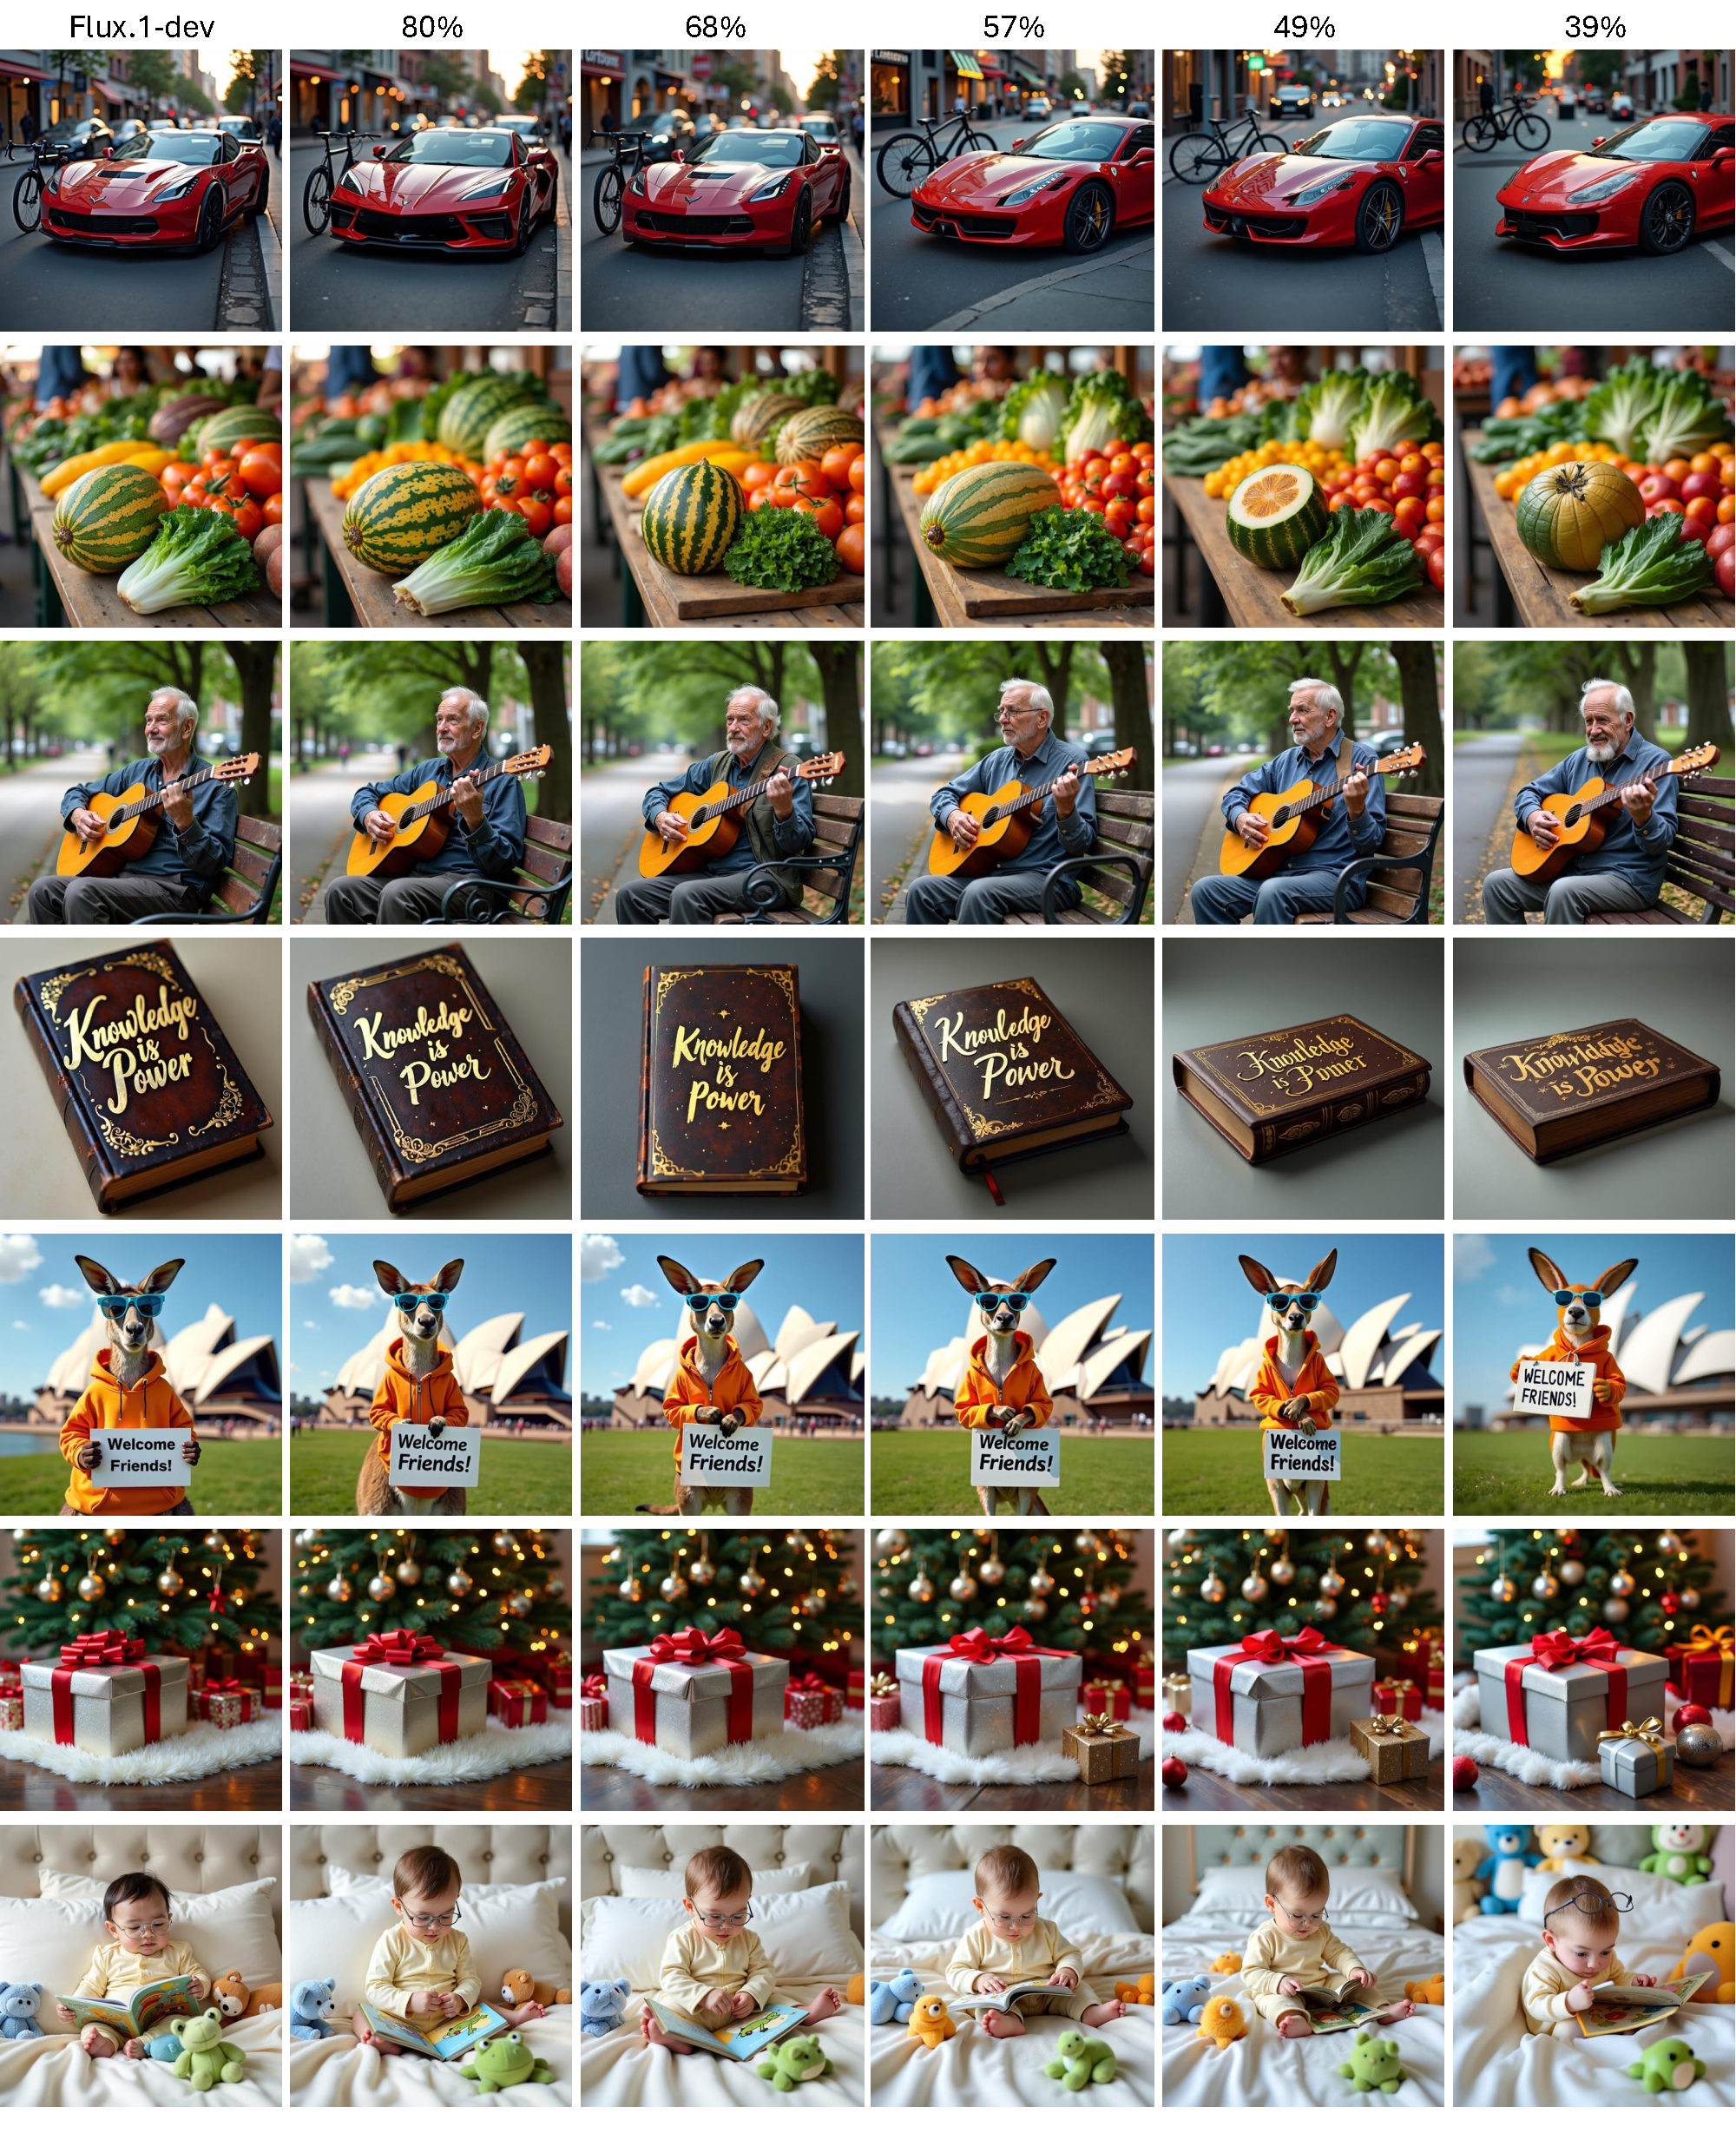
\includegraphics[width=\textwidth]{images/Experimente/Flux/SVDtrunc/Appendix_SVDtrunc.pdf}
	\caption[Qualitative Examples: SVDtrunc]{Qualitative comparison of example images generated by models compressed via SVDtrunc to varying sizes.}
	\label{fig:SVDtrunc_Appx}
\end{figure}


\subsubsection{Domain Shift}

\begin{figure}[H]
	\centering
	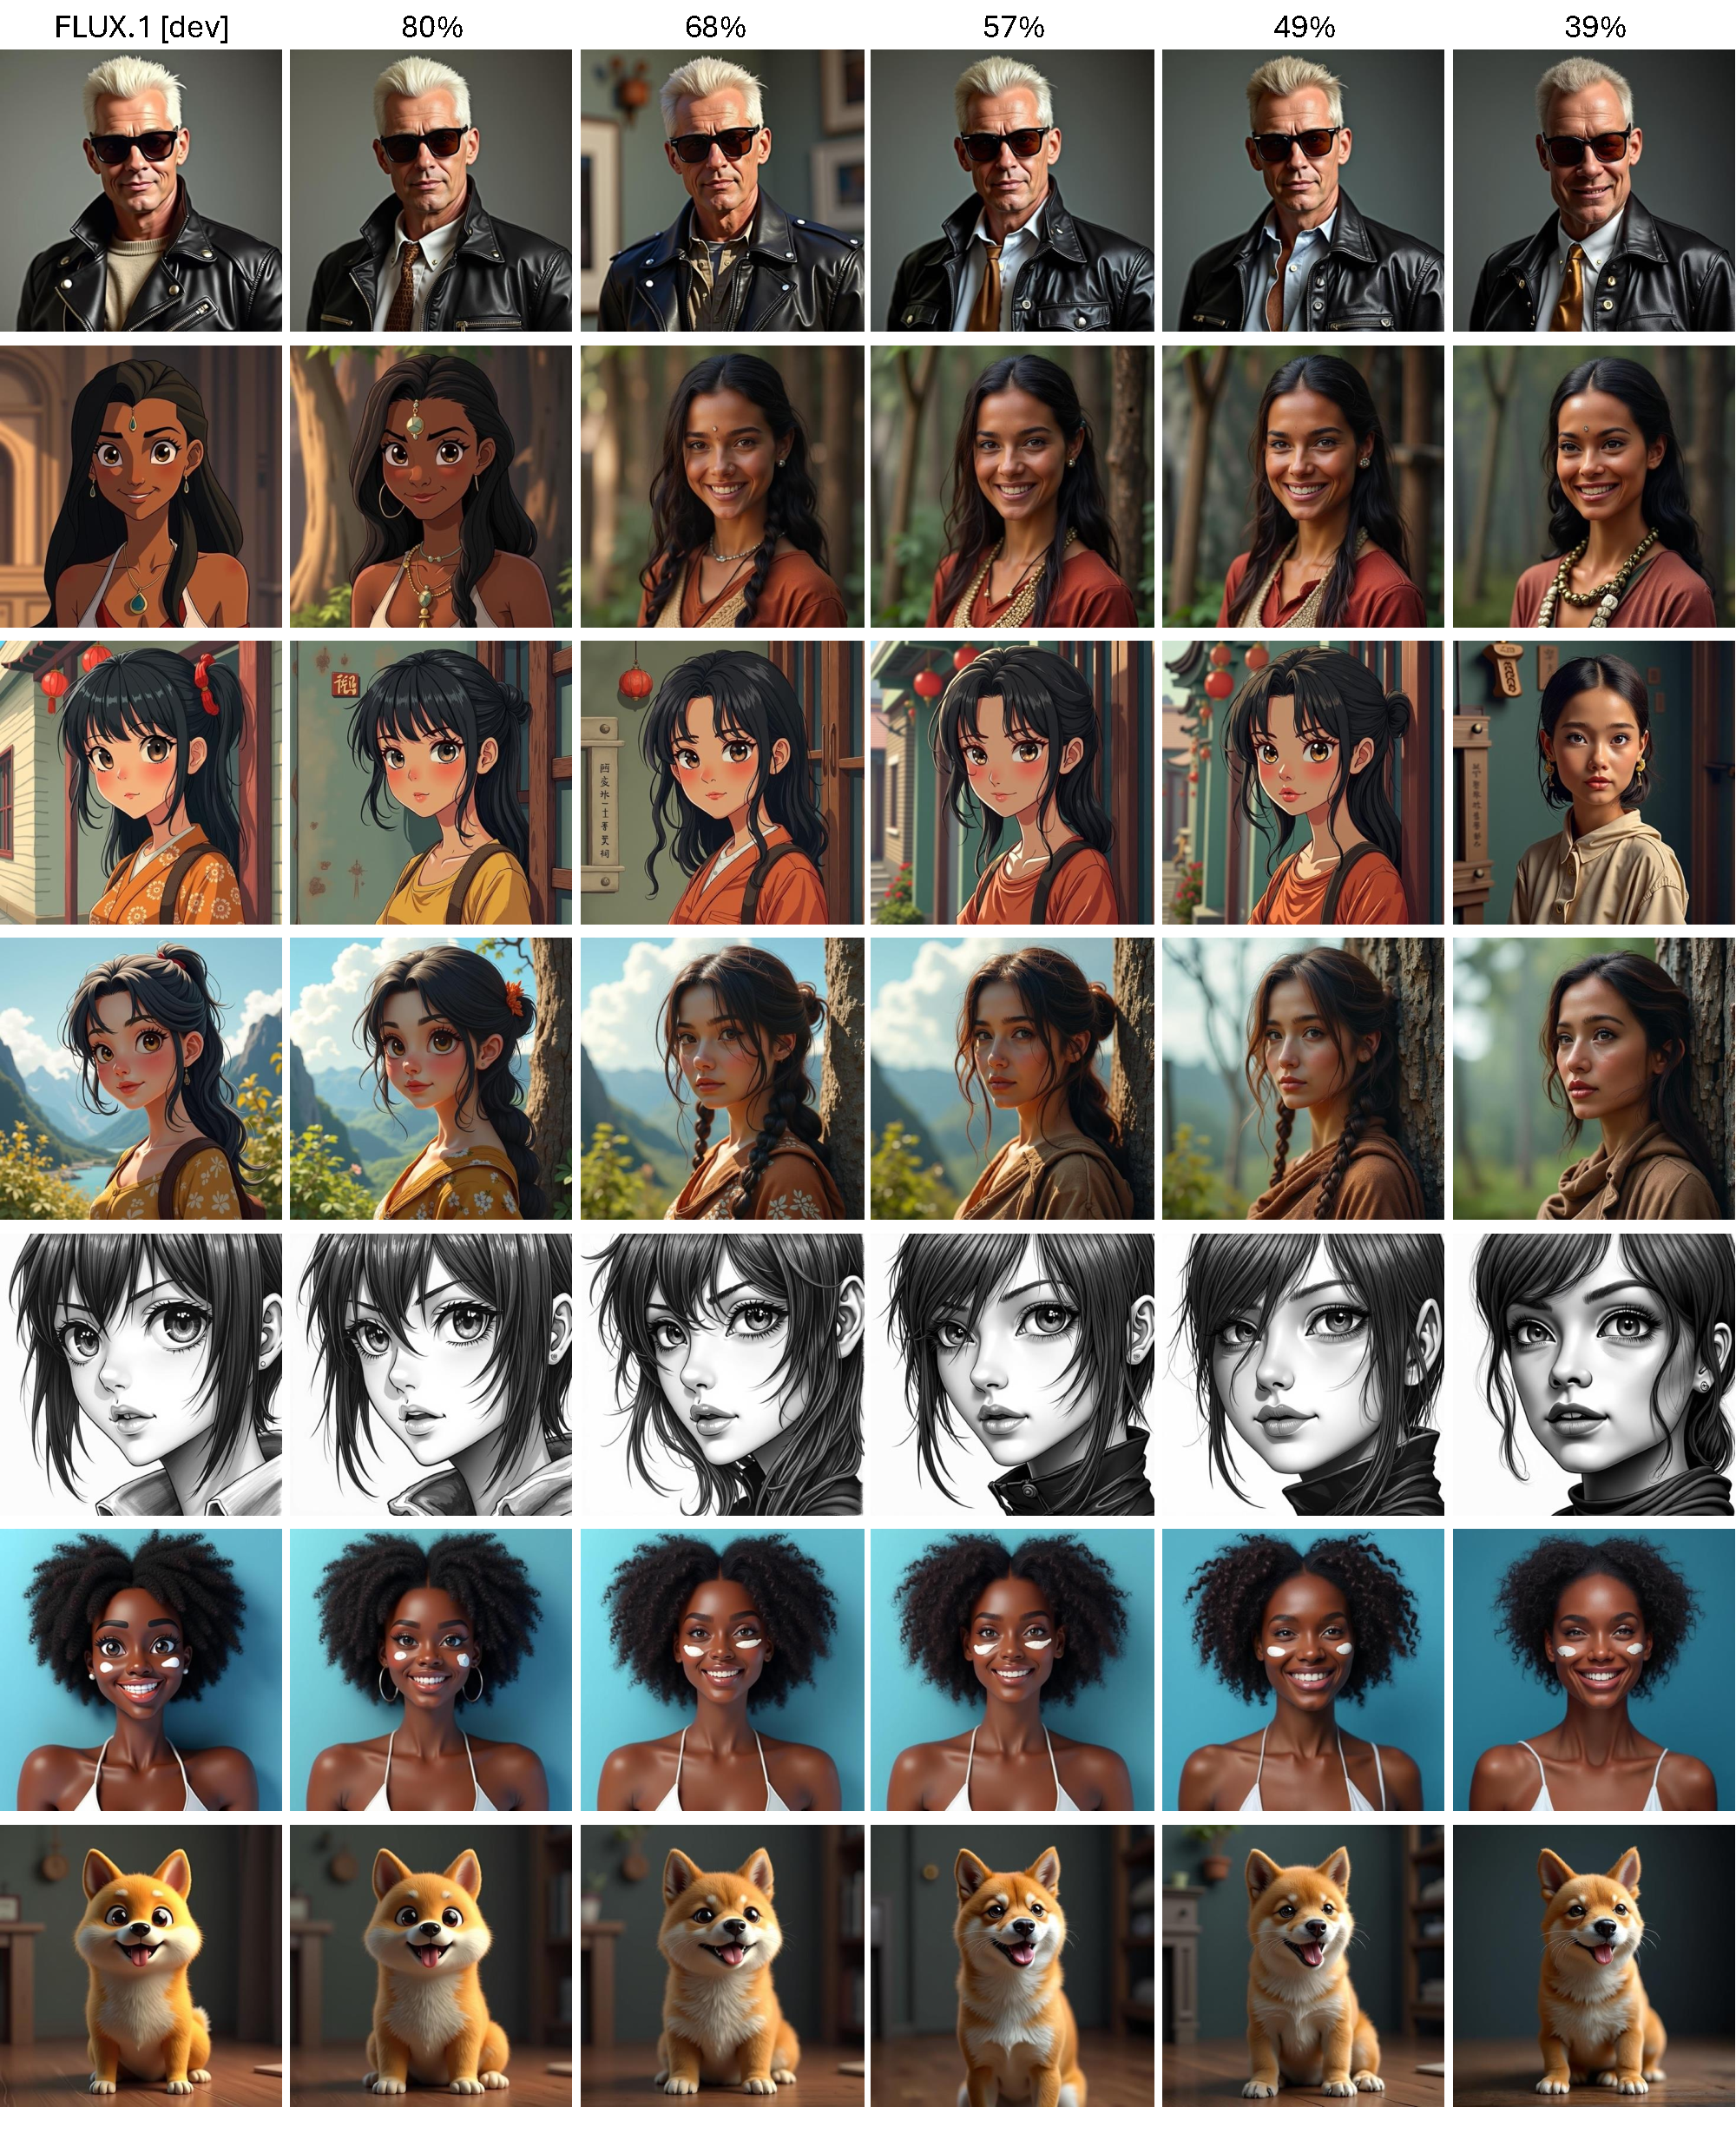
\includegraphics[width=\textwidth]{images/Experimente/Flux/SVDtrunc/Appendix_DomainShift.pdf}
	\caption[Qualitative Examples: Domain Shift in SVDtrunc]{Qualitative comparison of example images generated at varying compression ratios using SVDtrunc, illustrating the gradual domain-shift observed with increasing compression levels.}
	\label{fig:SVDtruncFlux_ShiftAppx}
\end{figure}

\begin{figure}[H]
	\centering
	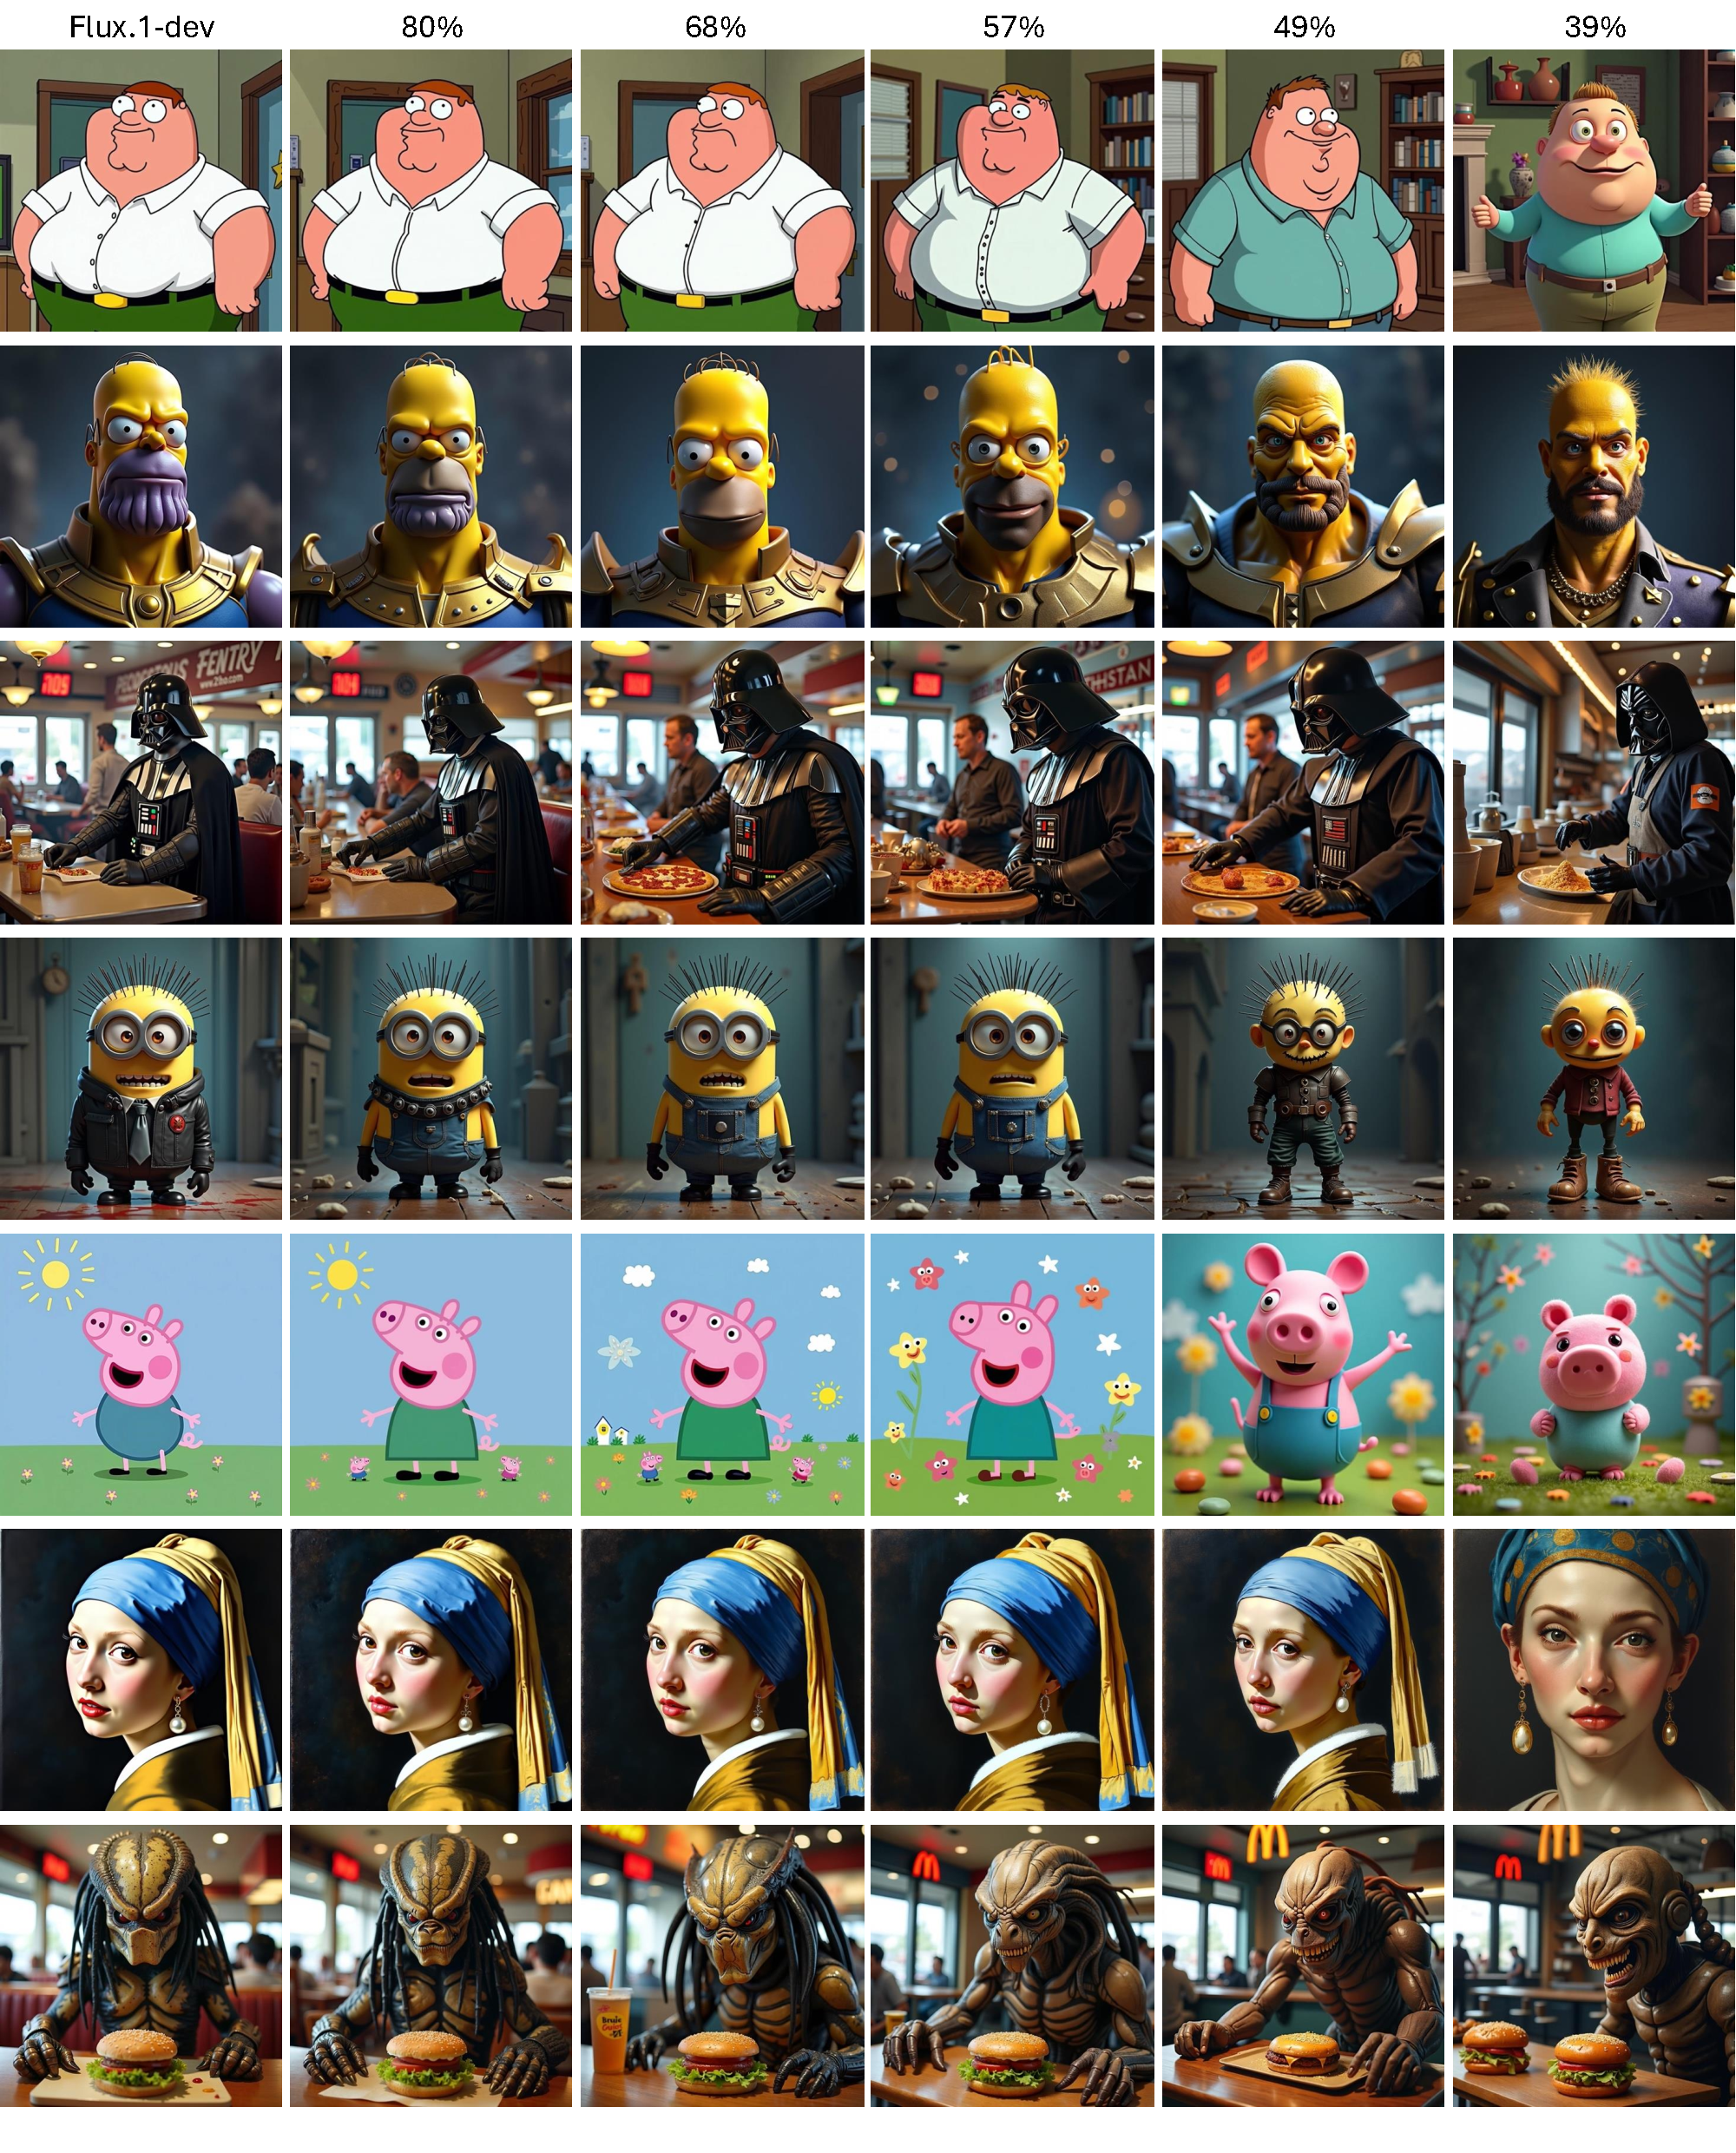
\includegraphics[width=\textwidth]{images/Experimente/Flux/SVDtrunc/Appendix_MemorizationLoss.pdf}
	\caption[Qualitative Examples: Memorization Loss in SVDtrunc]{Qualitative comparison of example images generated at varying compression ratios using SVDtrunc, illustrating the gradual memorization-loss observed with increasing compression levels.}
	\label{fig:SVDtrunc_Memorization_Loss_Appx}
\end{figure}


\subsubsection{Failure Cases}
Fig. \ref{fig:SVDtrunc_Failure_Cases_Appx} presents failure cases observed in highly compressed models. Note that all images were generated using the same seed on a A100 GPU. In rows 1 and 4, the images generated by the model retaining only 39\% of its original model size display a completely different motif. Row 1 shows a mosaic instead of a woman's face, and in row 4, a glowing object becomes an armored figure. Furthermore, the cyberpunk desk in row 5 entirely loses its 3D structure. In rows 2 and 3, the turtle becomes unrecognizable, and the hands and fingers of the students are displaced. Finally, the last row illustrates a complete mode collapse, where the model generates text blocks instead of the original 3D character.
\begin{figure}[H]
	\centering
	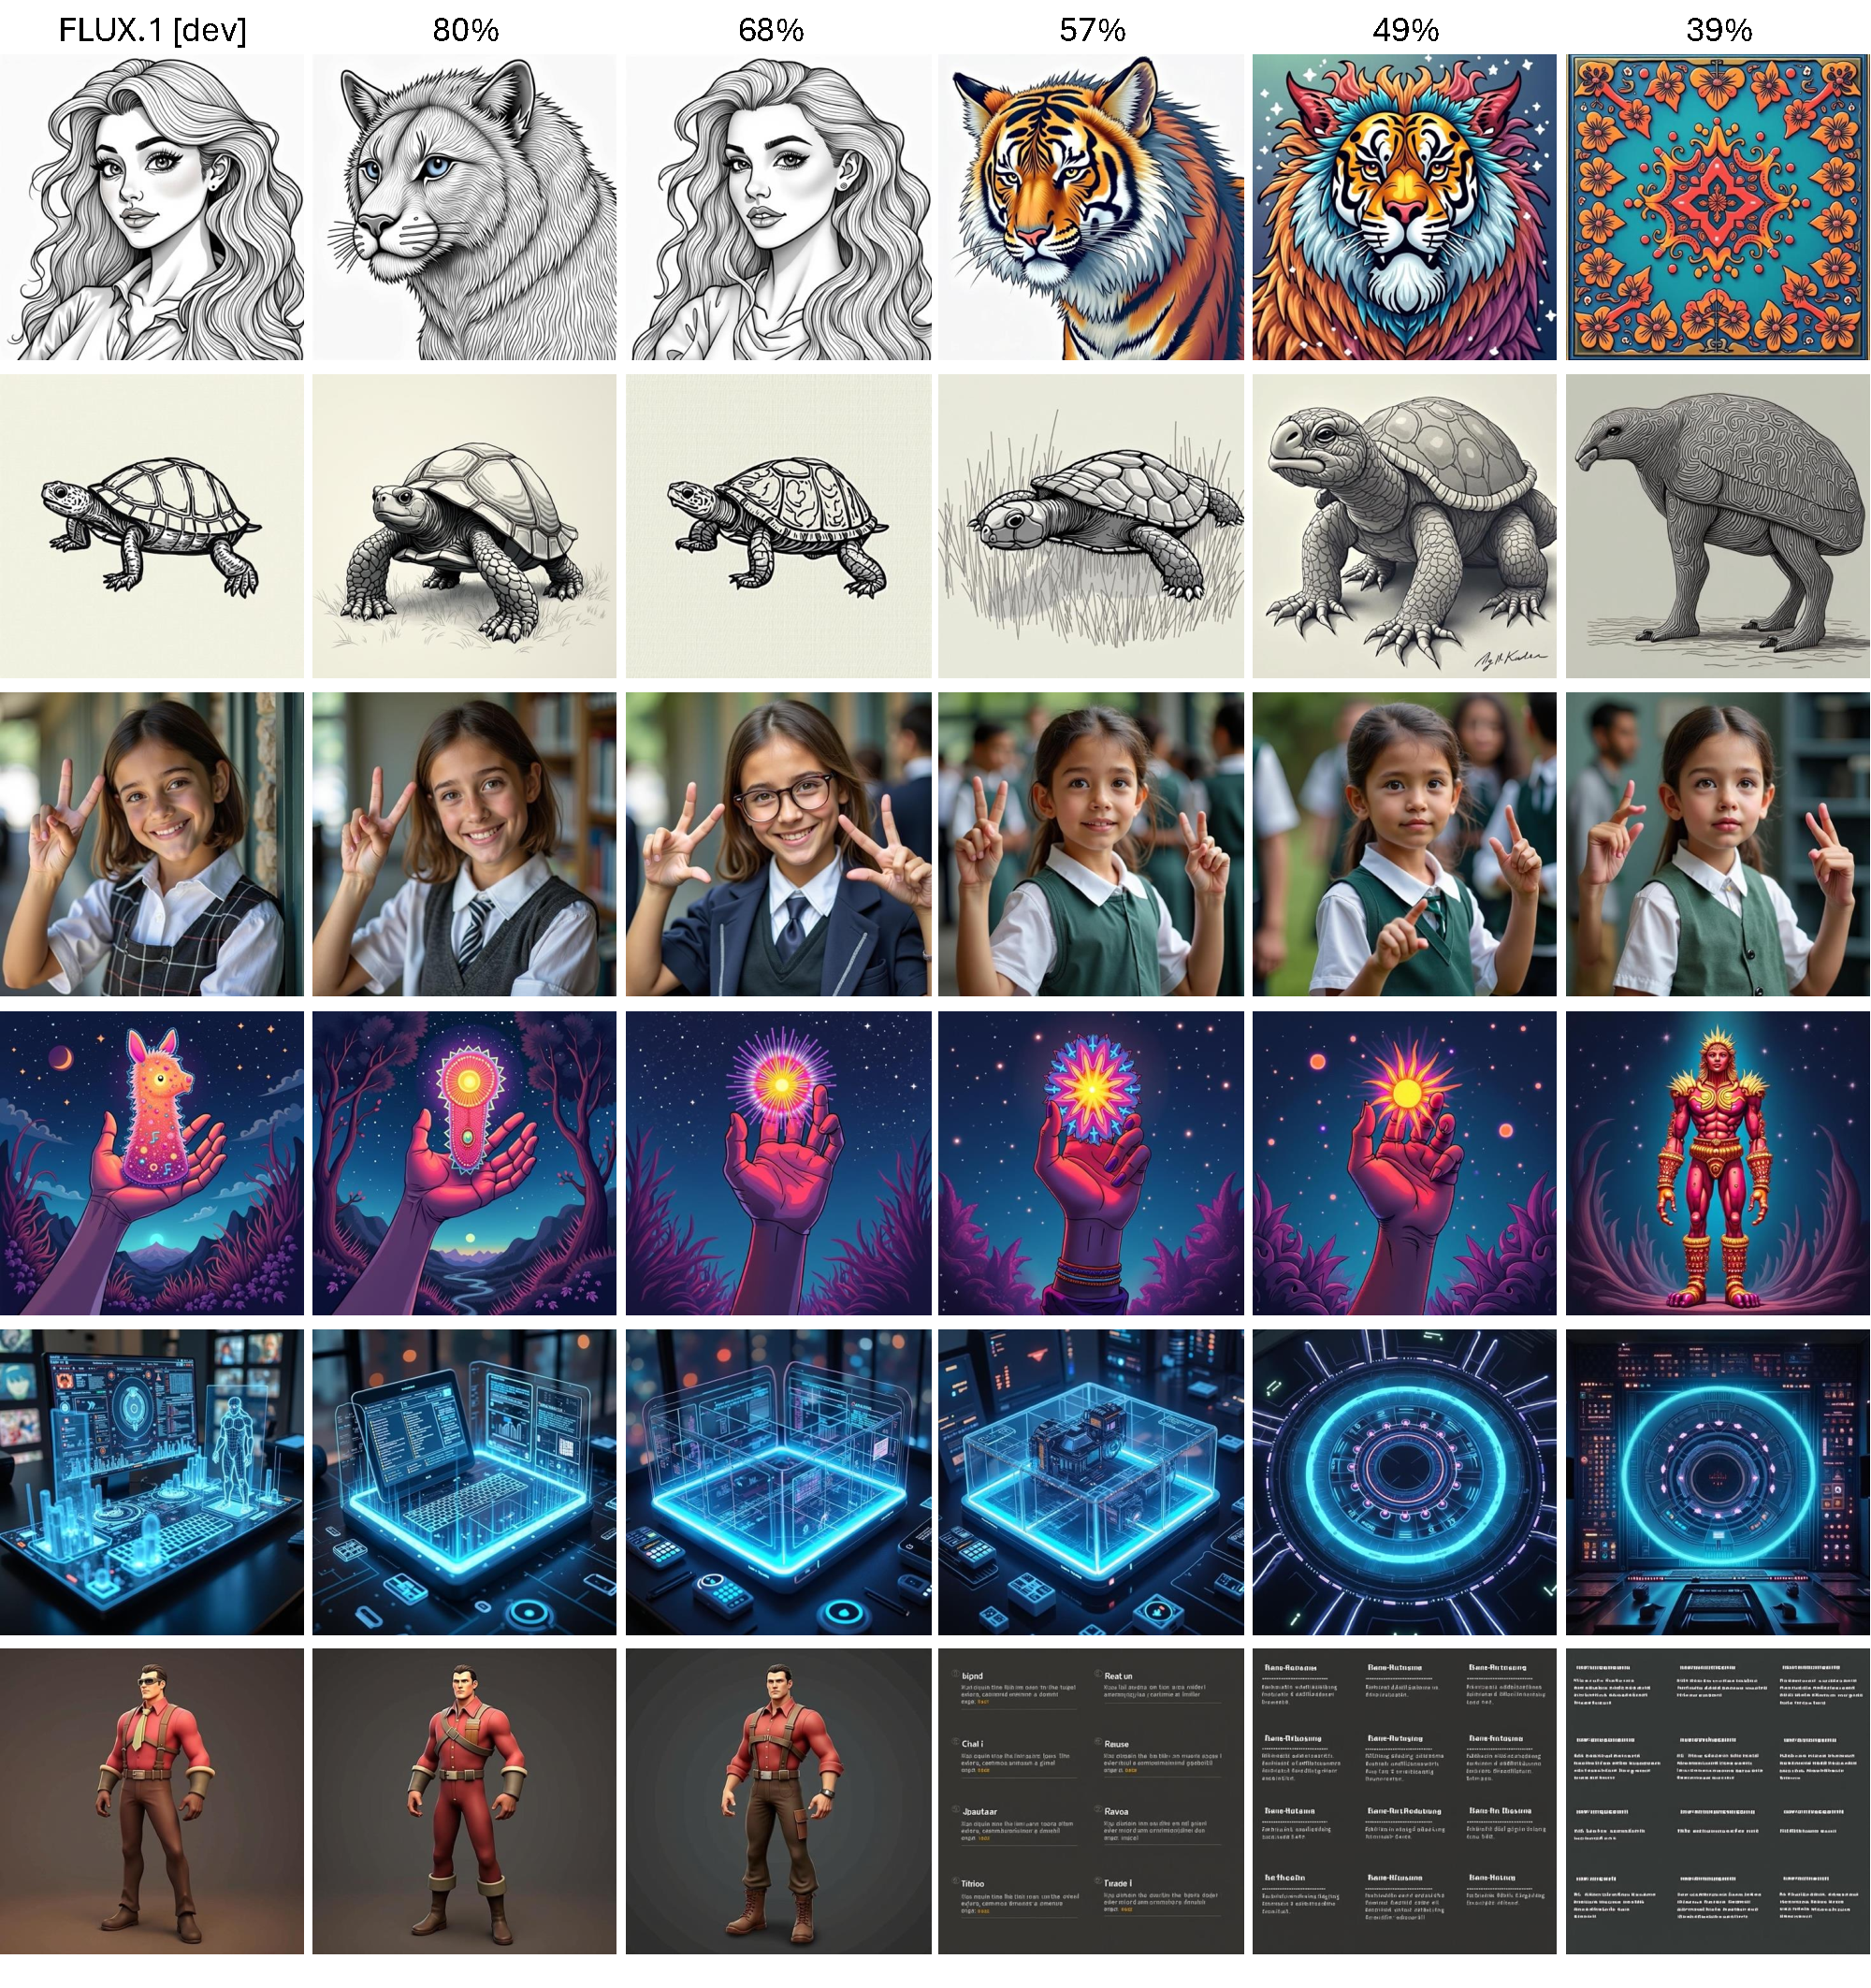
\includegraphics[width=\textwidth]{images/Experimente/Flux/SVDtrunc/Appendix_FailureCases.pdf}
	\caption[Qualitative Examples: Failure Cases in SVDtrunc]{Qualitative comparison of example images generated at varying compression ratios using SVDtrunc, illustrating failure cases observed with increasing compression levels.}
	\label{fig:SVDtrunc_Failure_Cases_Appx}
\end{figure}


\section{Evaluation SVDtrunc on Step-Distilled DiTs}
\label{appx:FluxSchnell}
This section provides additional qualitative example for FLUX.1 {[schnell]} (Sec. \ref{sec:FluxSchnellMainResults}) compressed via \gls{SVD}trunc (Fig. \ref{fig:FluxSchnellAppx}) as well as the compression details (Tab. \ref{tab:FluxDSchnell}). As with FLUX.1 {[dev]}, both domain shift (Fig. \ref{fig:FluxSchnellAppxDomainShift}) and memorization loss (Fig. \ref{fig:FluxSchnellAppxMemoLoss}) occur over the course of compression.






\begin{figure}[H]
	\centering
	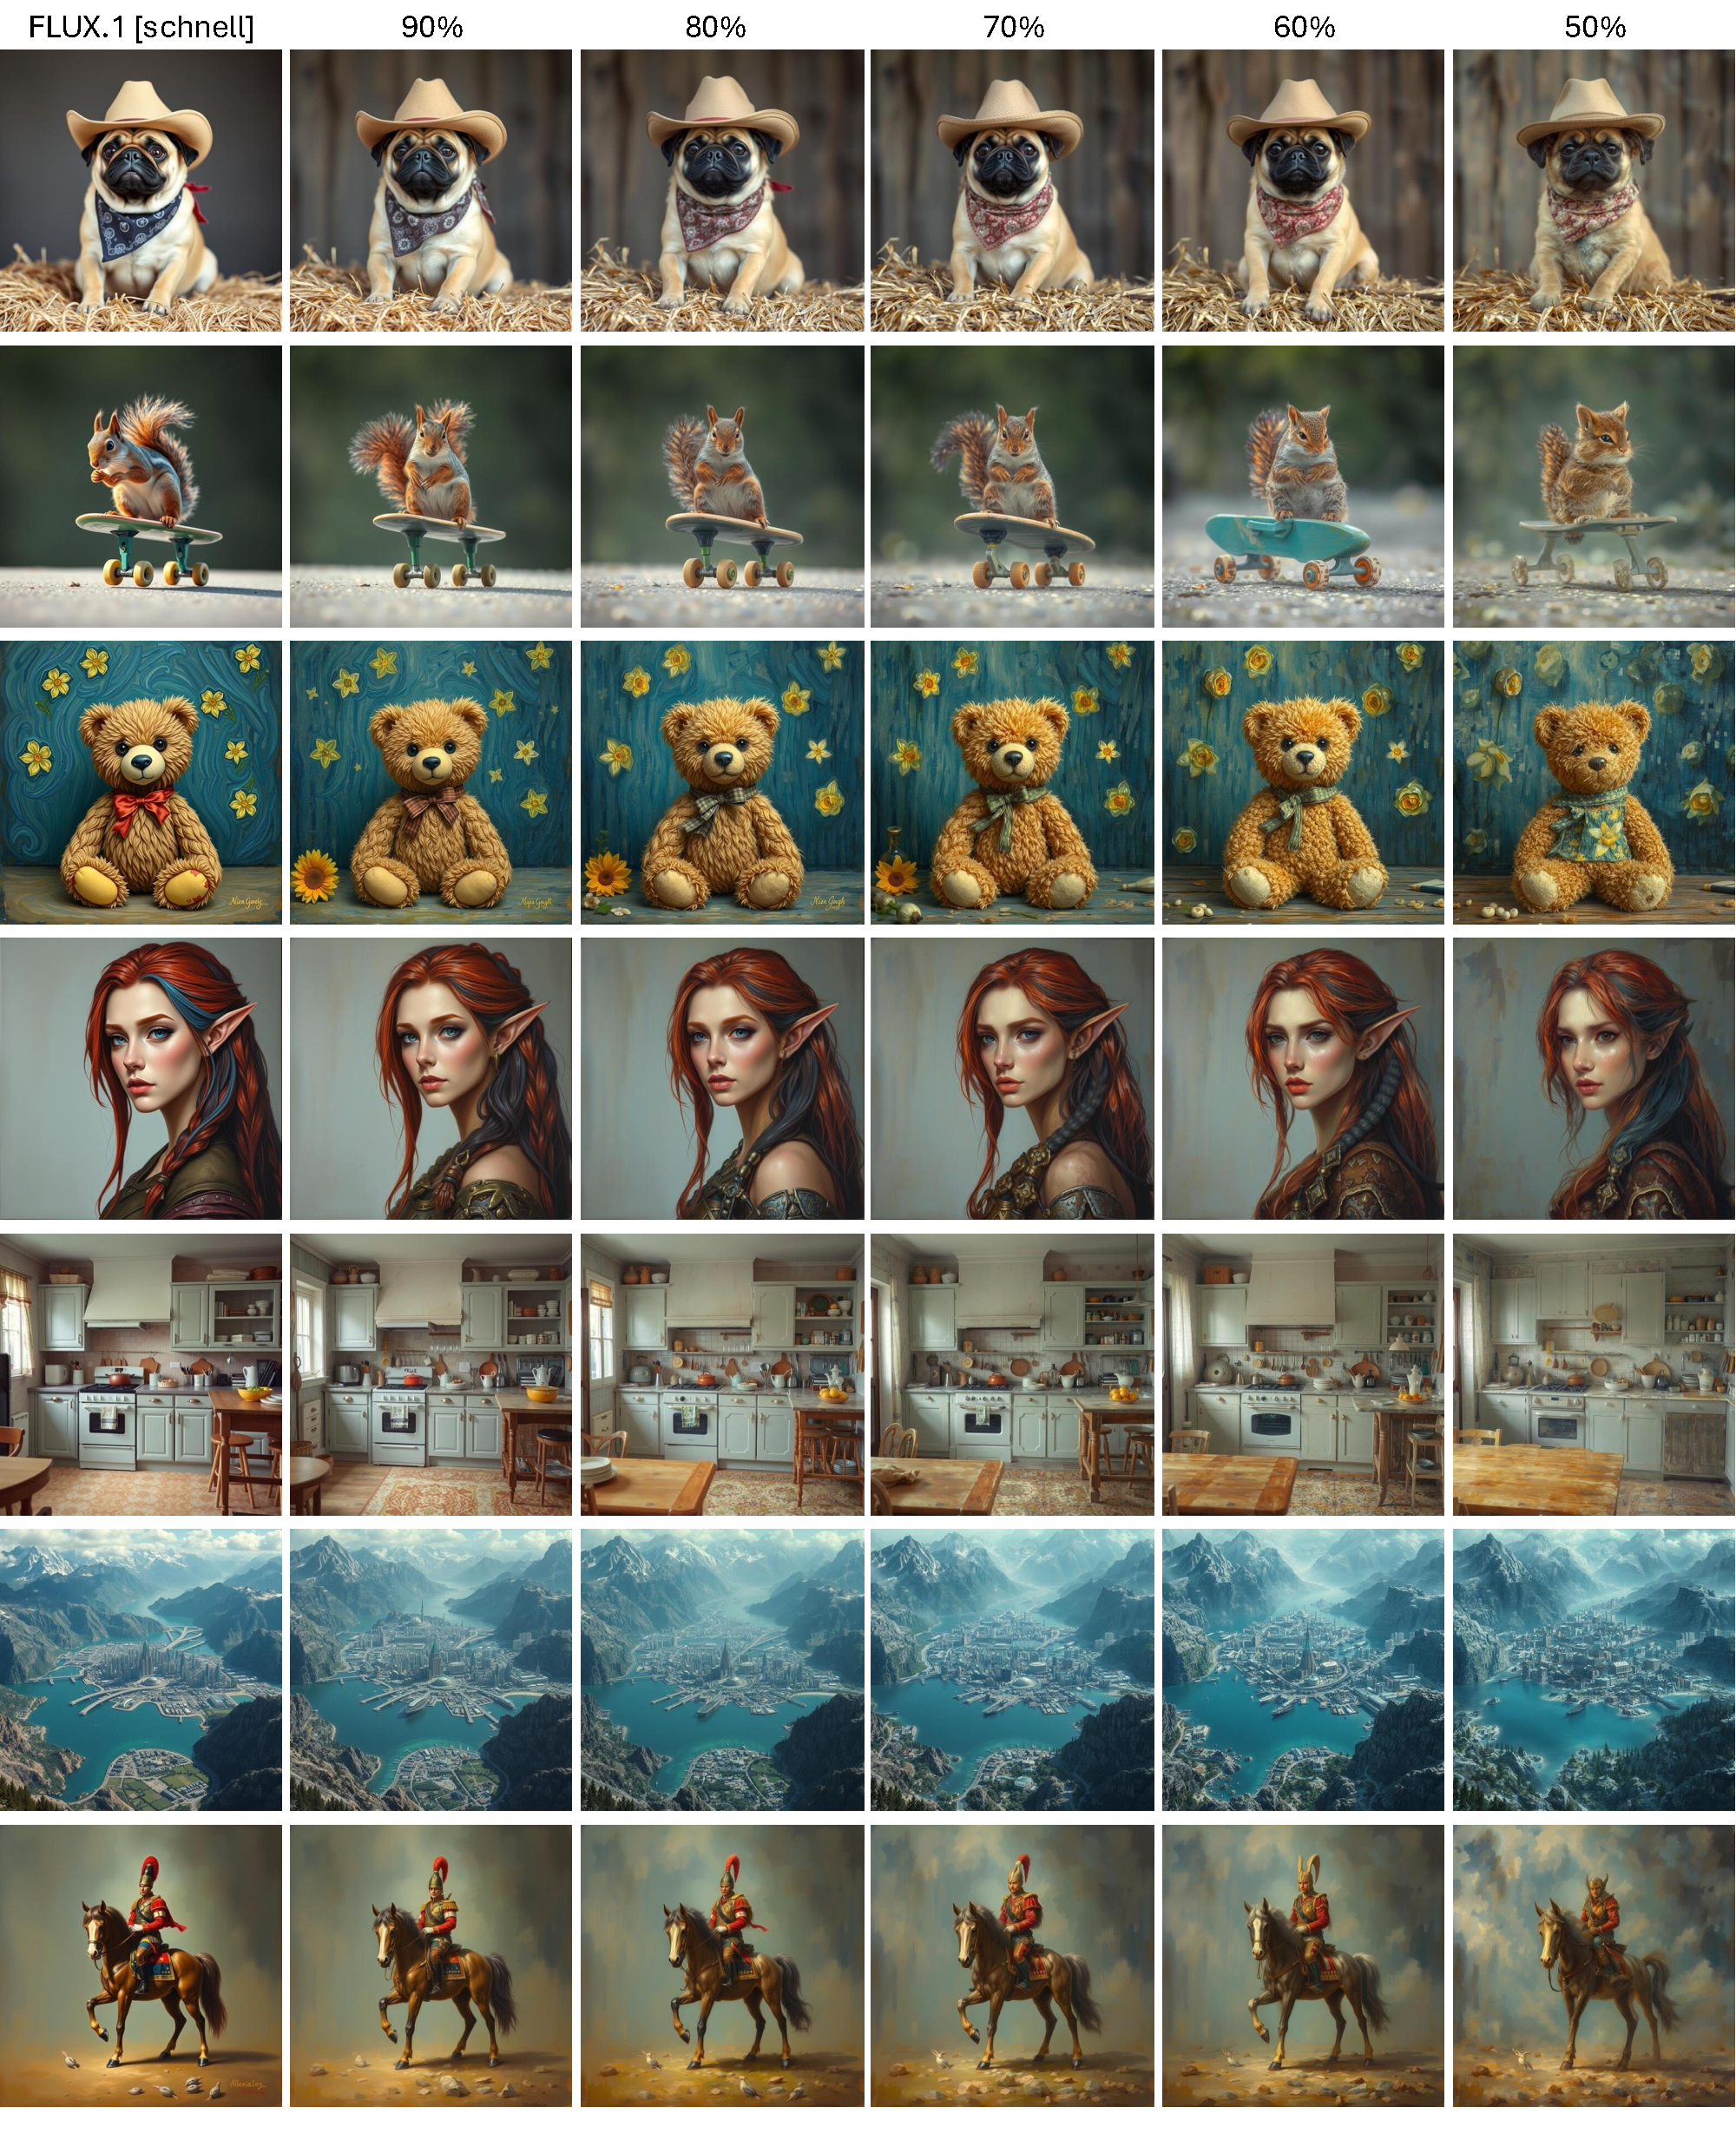
\includegraphics[width=0.9\textwidth]{images/Experimente/Flux/FluxSchnell/FluxSchnellAppx.pdf}
	\caption[Qualitative Examples: SVDtrunc on FLUX.1 {[schnell]}]{Qualitative comparison of example images generated by FLUX.1 {[schnell]} compressed via SVDtrunc to varying sizes utilizing four inference steps.}
	\label{fig:FluxSchnellAppx}
\end{figure}



\begin{figure}[H]
	\centering
	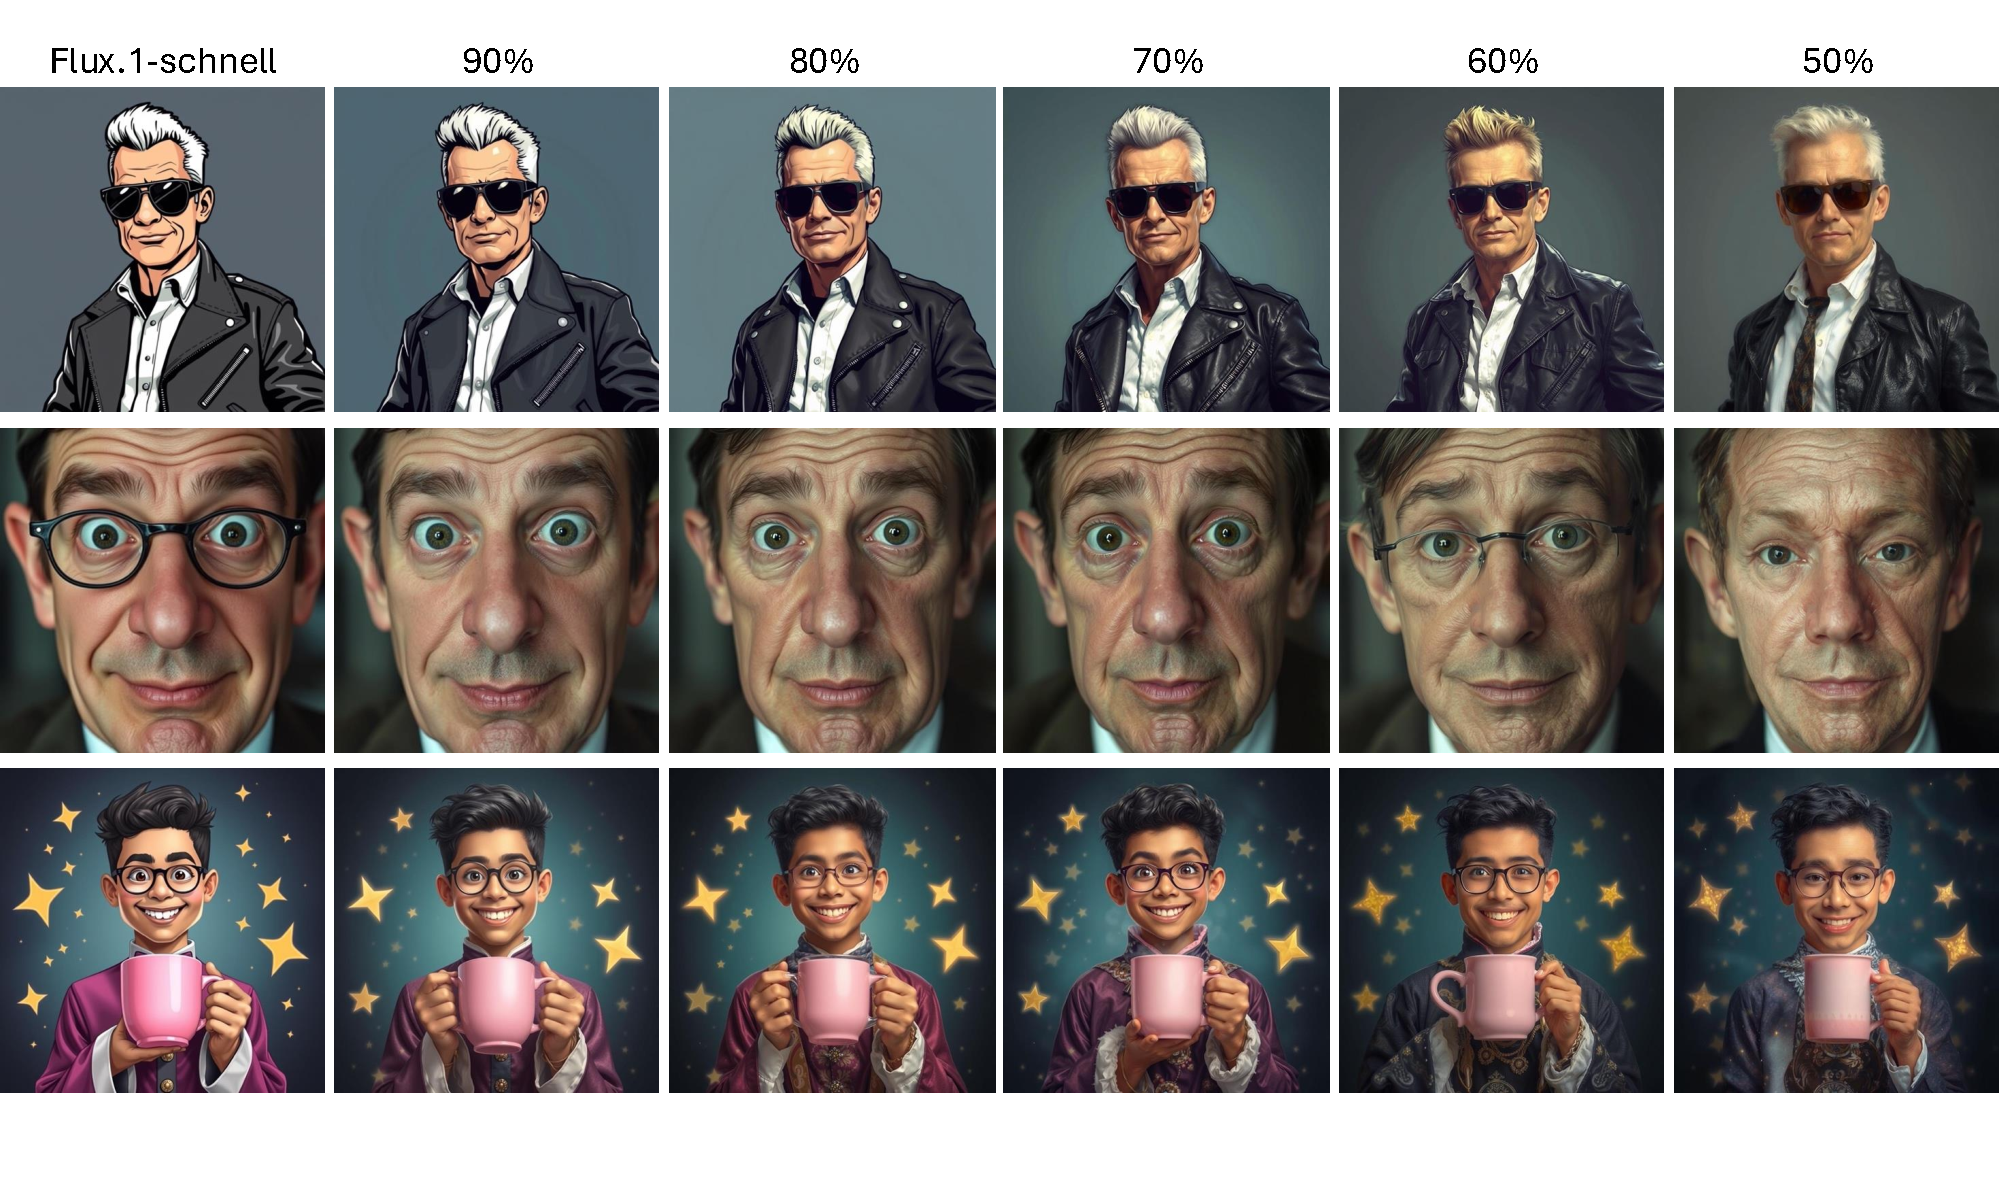
\includegraphics[width=0.9\textwidth]{images/Experimente/Flux/FluxSchnell/FluxSchnellDomainShift.pdf}
	\caption[Qualitative Examples: Domain Shift in SVDtrunc on FLUX.1 {[schnell]}]{Qualitative comparison of example images generated by FLUX.1 {[schnell]} compressed via SVDtrunc, illustrating the gradual domain-shift observed with increasing compression levels.}
	\label{fig:FluxSchnellAppxDomainShift}
\end{figure}

\begin{figure}[H]
	\centering
	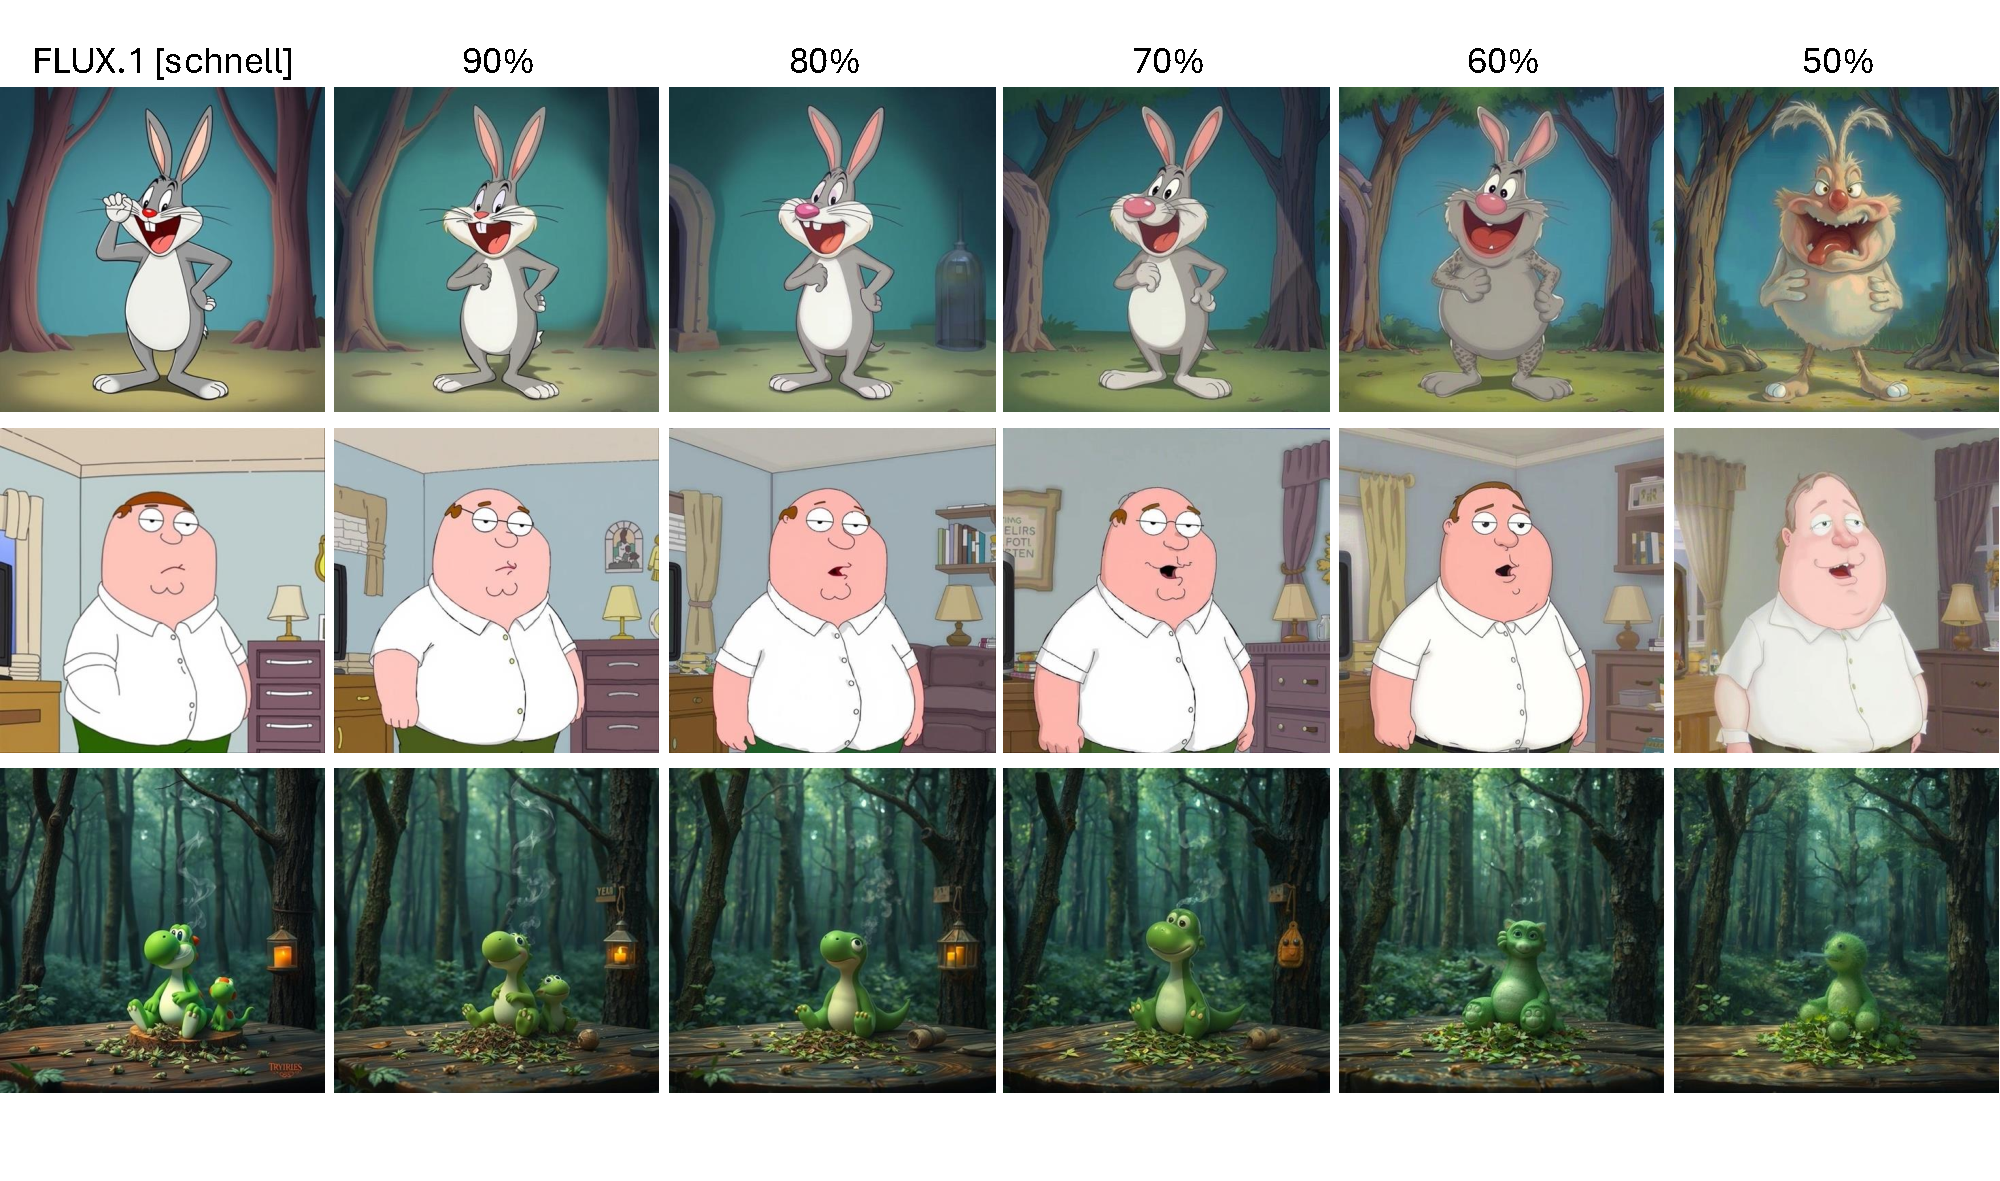
\includegraphics[width=0.9\textwidth]{images/Experimente/Flux/FluxSchnell/FluxSchnellMeMo.pdf}
	\caption[Qualitative Examples: Memorization Loss in SVDtrunc on FLUX.1 {[schnell]}]{Qualitative comparison of example images generated by FLUX.1 {[schnell]} compressed via SVDtrunc, illustrating the gradual memorization loss observed with increasing compression levels.}
	\label{fig:FluxSchnellAppxMemoLoss}
\end{figure}



\begin{table}[H]
	\centering
	\caption[SVDtrunc FLUX.1 {[schnel]}: Compression Details]{Overview of the experimental settings for the FLUX.1 [schnell] compression, detailing how the removed parameters are distributed across varying numbers of blocks. For readability, the linear decay rate $x$ is scaled by 1000.}
	\label{tab:FluxDSchnell}
	\begin{tabular}{cccccc}
		\toprule
		\textbf{Iteration} &\textbf{Model Size} & \textbf{Training Steps} & \textbf{Number of} & \textbf{Base Compression} & \textbf{Linear Decay}\\
		&&\textbf{Modified Blocks}&\textbf{Ratio}& \textbf{Rate} $x$\\
		\midrule
		
		1 &  90\%&  20,000 & 30 & 0.25 & 8.3 \\
		

		
		
		2 & 80\% & 20,000 &  30 & 0.25 & 5.9 \\
		
	
		
		3 & 70\% & 20,000 &  30 & 0.35  & 10.8 \\
		
	
		
		4& 60\% &  20,000 & 30 & 0.4  & 10.1 \\
		
	
		
		5& 50\%  &20,000 & 30  & 0.35 & 7.5  \\
		
		
		\bottomrule
	\end{tabular}
\end{table}




\section{Proof of Concept: GRASP for \gls{DiT}s}
The block importance ranking from \cite{FastFlux}, which was used in Sec. \ref{sec:GRASPForDiTs}, is shown in Fig. \ref{fig:GRAPSImportanceRanking}. Tab. \ref{tab:GRASPSVD_ranks} specifies the exact ranks used for the \gls{SVD} compression of the individual matrices within the double-stream blocks, and Tab. \ref{tab:GRASPpruned_blocks} lists the exact blocks that were compressed.
\subsubsection{Block Importance Ranking}
\label{app:GRASP_BlockImportance}
For this experiment the importance of blocks determined in \cite{FastFlux} was leveraged. Below the figure from the corresponding work is presented. 

\begin{figure}[htbp]
	\centering
	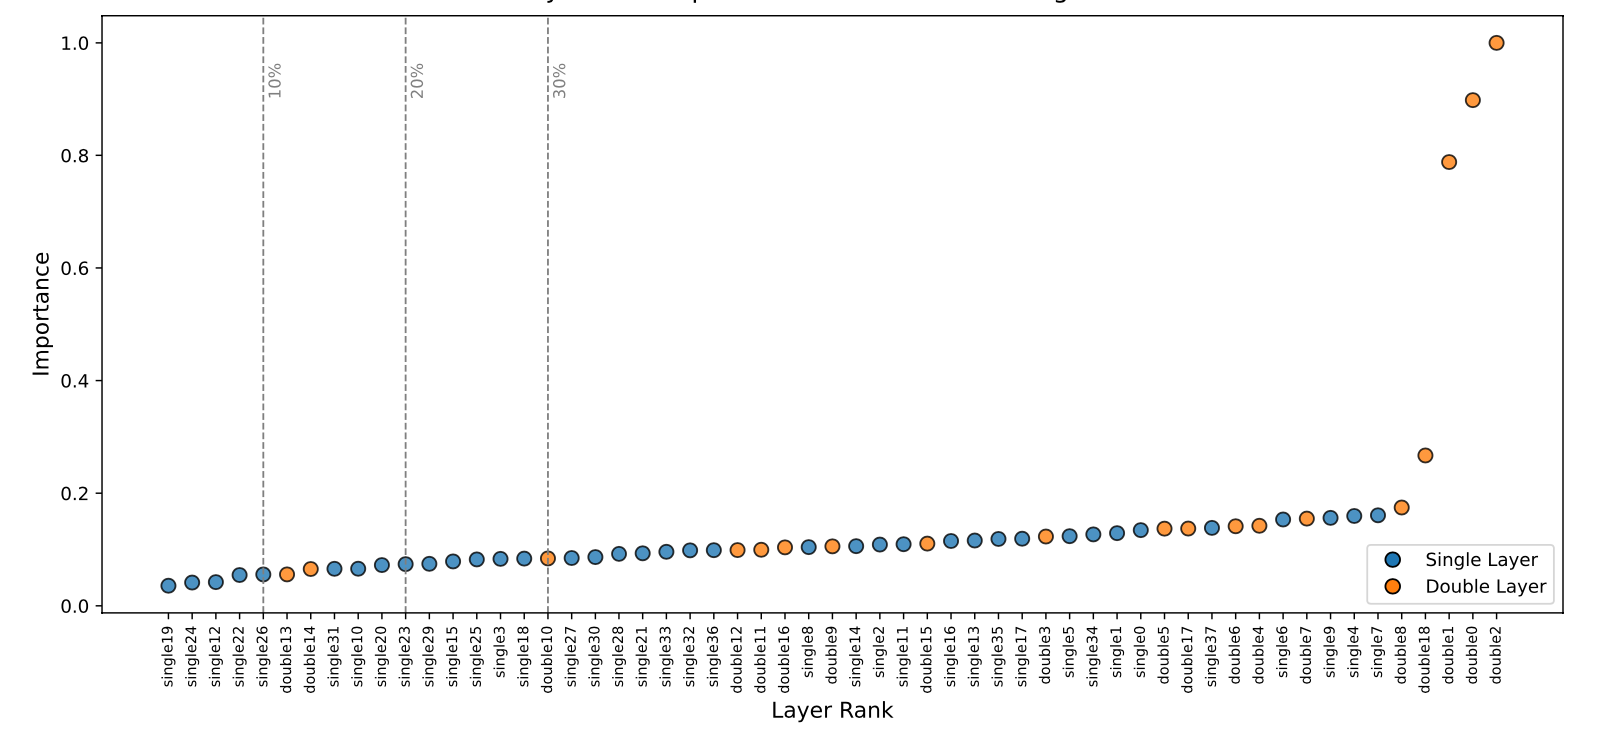
\includegraphics[width=0.9\textwidth]{images/Experimente/Flux/Training_Free/BlockImportanceFastFlux.png}
	\caption[GRASP: FLUX.1 {[dev]} Block Importance Ranking]{Block importance for FLUX.1 {[dev]} taken from \cite{FastFlux}.}
	\label{fig:GRAPSImportanceRanking}
\end{figure}

\subsubsection{Compression Details}
\begin{table}[H]
	
	\centering
	\caption[GRASP: \gls{SVD} Ranks]{Overview of compressed double-stream block components and the respecive rank used in \gls{GRASP}.}
	\label{tab:GRASPSVD_ranks}
	\begin{tabular}{l|c}
		\hline
		\textbf{Components Double Block} & \textbf{Rank for \gls{SVD}} \\ \hline
		Double-Stream Image Linear Layer (Attention) & $307$ \\
		Double-Stream Image MLP                      & $491$ \\
		Double-Stream Image Modulation               & $526$ \\
		Double-Stream Text Linear Layer (Attention)  & $307$ \\
		Double-Stream Text MLP                       & $491$ \\
		Double-Stream Text Modulation                & $526$ \\ \hline
	\end{tabular}
\end{table}

\begin{table}[H]
	\centering
	\caption[GRASP: Model Compression Configuration]{Overview of compressed double-stream block configurations.}
	\label{tab:GRASPpruned_blocks}
	\begin{tabular}{l c p{6cm}}
		\toprule
		\textbf{Model Size} & \textbf{Modified Blocks} & \textbf{Compressed Double-Stream Block IDs} \\
		\midrule
		80\% & 9 & 13, 14, 10, 12, 11, 16, 9, 15, 3 \\
		74\% & 12 &  13, 14, 10, 12, 11, 16, 9, 15, 3, 5, 17, 6 \\
		68\% & 15 & 13, 14, 10, 12, 11, 16, 9, 15, 3, 5, 17, 6, 4, 7, 8 \\
		60\% & 18 & 13, 14, 10, 12, 11, 16, 9, 15, 3, 5, 17, 6, 4, 7, 8, 18, 1, 0  \\
		\bottomrule
	\end{tabular}
\end{table}